\documentclass[12pt,a4paper,oneside]{book} % twoside for draf

% \usepackage[utf8]{vietnam}
%\usepackage{times}
\usepackage{svg}
\usepackage{graphicx}
\usepackage{subcaption}
\usepackage{float}
\usepackage{makecell}
\usepackage{mathptmx}	% same Time New Roma
%\renewcommand{\rmdefault}{phv} % Arial
%\renewcommand{\sfdefault}{phv} % Arial
\usepackage{url}
\usepackage{setspace}
\usepackage[numbers, sort&compress]{natbib}
\usepackage[utf8]{inputenc}
\usepackage[vietnamese]{babel}
%link to part by click on contents region
\usepackage{hyperref}
\hypersetup{
    colorlinks,
    citecolor=black,
    filecolor=black,
    linkcolor=black,
    urlcolor=black
}

\usepackage{fancyhdr}
\usepackage{algorithm2e}
\usepackage{amsmath}
\usepackage{array,tabularx}
\usepackage{amsfonts}
\usepackage{amssymb}
\usepackage{cases}
\usepackage{tabularx}
\usepackage{adjustbox}
\usepackage{multirow}
\usepackage{acronym} 
\usepackage{bkthesis}
\usepackage{tikz}
\usepackage{colortbl}
\usepackage[normalem]{ulem}
\useunder{\uline}{\ul}{}
\usepackage{adjustbox}
\usetikzlibrary{shapes,arrows}
\newenvironment{conditions*}
  {\par\vspace{\abovedisplayskip}\noindent
   \tabularx{\columnwidth}{>{$}l<{$} @{${}:{}$} >{\raggedright\arraybackslash}X}}
  {\endtabularx\par\vspace{\belowdisplayskip}}

\tikzstyle{blank} = [text badly centered, node distance = 2cm, inner sep=0pt]
\tikzstyle{block} = [rectangle, draw, 
    text width=2em, text centered, minimum height=2em]
\tikzstyle{line} = [draw, -latex']

\newcolumntype{b}{>{\hsize=1.0\hsize}X}

\crname{BÁO CÁO LUẬN VĂN TỐT NGHIỆP}
\ctname{CẢI THIỆN ĐỊNH VỊ TRỰC QUAN VỚI HƯỚNG TIẾP CẬN HỌC SÂU}
\cstuname{
\begin{tabular}{ l l l}
	SVTH 1: & Lê Minh Nghĩa & 2010445\\
	SVTH 2: & Phạm Khai Anh Duy & 2011015\\
  SVTH 3: & Nguyễn Trọng Nhân & 2011744
\end{tabular}
}

\csCouncil{5}
\csSupervise{TS. Nguyễn Đức Dũng}
\csReviewer{Vũ Văn Tiến}
\cttime{05/2024}

\thesislayout
\begin{document}
%-	Bìa cứng - màu xanh dương, chữ mạ vàng (xem mẫu đính kèm)
%-	Trang tên (tờ lót): chất liệu giấy, nội dung giống như bìa LV
%-	Ở gáy LV: in nhan đề LV (có thể in tóm tắt nếu nhan đề quá dài), size 15 – 17
%-	Phiếu Nhiệm vụ LV, chấm điểm Hướng dẫn & Phản biện (đã ký): nhận từ GVHD & GVPB sau khi bảo vệ (theo lịch hẹn).
%-	Lời cam đoan
%-	Lời cảm ơn/ Lời ngỏ
%-	Tóm tắt LV
%-	Mục lục
%-	Danh mục, bảng biểu, hình ảnh, ... (nếu có)
%-	Nội dung LV
%-	Danh mục TL tham khảo
%-	Phụ lục (nếu có)

\coverpage

\frontmatter

% add content here
%-	Lời cam đoan
\begin{declaration}
Chúng tôi xin cam đoan đây là công trình nghiên cứu của riêng chúng tôi dưới sự hướng dẫn của TS. Nguyễn Đức Dũng. Nội dung nghiên cứu và các kết quả đều là trung thực và chưa từng được công bố trước đây. Các số liệu được sử dụng cho quá trình phân tích, nhận xét được chính chúng tôi thu thập từ nhiều nguồn khác nhau và sẽ được ghi rõ trong phần tài liệu tham khảo.

Ngoài ra, chúng tôi cũng có sử dụng một số nhận xét, đánh giá và số liệu của các tác giả khác, cơ quan tổ chức khác. Tất cả  đều có trích dẫn và chú thích nguồn gốc.

Nếu phát hiện có bất kì sự gian lận nào, chúng tôi xin hoàn toàn chịu trách nhiệm về nội dung đồ án tốt nghiệp của mình. Trường Đại học Bách Khoa Thành phố Hồ Chí Minh không liên quan đến những vi phạm tác quyền, bản quyền do chúng tôi gây ra trong quá trình thực hiện.

\end{declaration}
~
\begin{acknowledgments}

    Luận văn tốt nghiệp được hoàn thành dưới sự hướng dẫn khoa học của TS. Nguyễn Đức Dũng, Khoa Khoa học và Kỹ Thuật Máy Tính, Trường Đại học Bách Khoa - Đại học Quốc gia Thành phố Hồ Chí Minh. Chúng tôi xin chân thành cảm ơn TS. Nguyễn Đức Dũng, đã giúp đỡ chúng tôi về kiến thức chuyên môn, thảo luận, đưa ra gợi ý và tạo điều kiện thuận lợi cho chúng tôi hoàn thành luận văn.

    Chúng tôi cũng xin gửi lời cảm ơn đặc biệt đến quý thầy cô phản biện, những người đã đọc và đóng góp ý kiến để chúng tôi hoàn thiện đồ án chuyên ngành của mình. Chúng tôi cũng xin bày tỏ lòng biết ơn sâu sắc đến quý thầy cô khoa Khoa học và Kỹ Thuật Máy tính, Trường Đại học Bách Khoa - Đại học Quốc gia Thành phố Hồ Chí Minh, là những người đã truyền thụ kiến thức chuyên môn, đã tạo điều kiện cho chúng tôi học tập và phát triển trong suốt quãng thời gian vừa qua.

    Kính chúc quý thầy cô sức khoẻ, thành công và tiếp tục đào tạo những thế hệ sinh viên mới trong tương lai.

    Chúng tôi xin chân thành cảm ơn.

    \begin{flushright}
        \textbf{Nhóm thực hiện} \\
        Lê Minh Nghĩa \\
        Phạm Khai Anh Duy \\
        Nguyễn Trọng Nhân \\
    \end{flushright}

\end{acknowledgments}
~
\begin{abstract}

    Khả năng định vị toàn cầu đóng vai trò cốt lõi trong những lĩnh vực phụ thuộc vào việc nhận biết và tương tác với môi trường xung quanh như xe tự hành, robot và công nghệ thực tế ảo AR. Trước đây, những công nghệ này sẽ phụ thuộc vào những hệ thống định vị toàn cầu như GPS. Tuy nhiên, công nghệ này vẫn còn những giới hạn nhất định về độ chính xác vị trí cũng như không xác định được hướng xoay. Để đáp ứng nhu cầu ngày càng tăng về độ chuẩn xác, bài toán định vị trực quan - Visual Localization - đã ra đời với mục tiêu thông qua việc thu thập dữ liệu trực quan tại một khu vực nhất định, chúng ta có thể định vị chính xác vị trí cũng như hướng nhìn của một người tại khu vực đó.

    Trong các các hướng tiếp cận hiện đại, nhận thấy các mô hình định vị trực quan cổ điển và định vị trực quan bằng phương pháp hồi quy thường đề xuất các mô hình có tác động tài nguyên huấn luyện lớn và khó phát triển về mặt phạm vi sử dụng, chúng tôi chia bài toán định vị trực quan thành một quy trình hai bước - nhận diện địa điểm trực quan (Visual Place Recognition) và ước tính vị trí của máy ảnh tương đối (Relative Pose Estimation). Trong quá trị nhận dạng địa điểm trực quan, mô hình sẽ nhận vào một ảnh truy vấn và chọn ra một hay nhiều ảnh từ tập ảnh được cung cấp, thể hiện cùng một cảnh với ảnh đầu vào. Từ cặp ảnh truy vấn và ảnh tham khảo đầu vào, mô hình sẽ tính toán vị trí và hướng quay của máy ảnh trong không gian.

    Nhận thấy rằng mỗi bước của bài toán khi hoạt động riêng lẻ đều có những điểm mạnh cũng như những hạn chế riêng, chúng tôi đặt ra mục tiêu nghiên cứu cấu trúc của mô hình và đề xuất phương hướng phát triển để kết hợp hai bước xử lý thành một quy trình hoàn chỉnh, nhằm bổ trợ cho những khiếm khuyết của mỗi bước, với mục đích cuối cùng là xây dựng một mô hình định vị trực quan hoạt động trên cả phạm vi nhỏ lẫn phạm vi rộng như thành thị. Kiến trúc của chúng tôi sử dụng hai mô hình:

    \begin{itemize}
        \item MixVPR \cite{alibey2023mixvpr}, được phát triển bởi Ali-bey và những cộng sự vào năm 2023, cho bước nhận diện địa điểm trực quan, hỗ trợ đưa mô hình định vị lên phạm vị không gian rộng lớn.
        \item Mô hình ước tính vị trí máy ảnh 2D-2D được đề xuất trong Map-free Relocalization \cite{arnold2022mapfree}, phát triển bởi Arnold và những cộng sự vào năm 2022, hỗ trợ tính toán vị trí và hướng quay chính xác của máy ảnh trong không gian từ mỗi cặp ảnh.
    \end{itemize}

\end{abstract}
% sử dụng các phần bên dưới nếu cần:
\tableofcontents
%\listofsymbols
\listoftables
\listoffigures

%\listofalgorithms
~

\titlepage \null
	\small
	\begin{center}
	  {\bfseries Bảng những từ ngữ chuyên ngành được sử dụng và phiên bản tiếng Anh\vspace{-.5em}}
	\end{center}
	\quotation
\begin{table}[h]
\centering
\begin{tabular}{|c|c|c|}
\hline
\textbf{STT} & \textbf{Bản tiếng Việt}                & \textbf{Bản tiếng Anh}     \\ \hline
1            & Bản địa hóa trực quan                  & Visual Localization        \\ \hline
2            & Ước tính vị trí máy ảnh                & Camera Pose Estimation     \\ \hline
3            & Hồi quy vị trí tuyệt đối               & Absolute Pose Regression   \\ \hline
4            & Hồi quy vị trí tương đối               & Relative Pose Regression   \\ \hline
5            & Máy ảnh lỗ kim                         & Pinhole Camera             \\ \hline
6            & Ma trận thiết yếu                      & Essential Matrix           \\ \hline
7            & Tìm sự tương ứng giữa đặc trưng ảnh    & Feature Matching           \\ \hline
8            & Giải thuật 5 điểm ảnh                  & 5-Point Solver             \\ \hline
9            & Thuật toán tính độ sâu ảnh qua một ảnh & Monocular Depth Estimation \\ \hline
10           & Truy xuất ảnh                          & Image Retrieval            \\ \hline
11           & Bản đồ đám mây điểm 3D                          & 3D point cloud            \\ \hline
12           & Tái tạo kiến trúc từ chuyển động                          & Structure from Motion            \\ \hline
13           & Mạng Nơ-ron tích chập                         & Convoluted Neural Network           \\ \hline
14           & Trích xuất đặc trưng ảnh                         & Feature Extraction           \\ \hline
15           & Đặc trưng ảnh cục bộ                         & Local Descriptor           \\ \hline
16           & Đặc trưng ảnh toàn cục                         & Global Descriptor           \\ \hline
17           & Bản đồ đặc trưng ảnh                         & Feature Map           \\ \hline
18           & Lớp pha trộn đặc trưng ảnh                         & Feature Mixer           \\ \hline
19          & Lớp kết nối đầy đủ        & Fully Connected Layer \\ \hline
20          & Bộ nhớ dài-ngắn hạn       & Long Short Term Memory \\ \hline
21          & \makecell{Hồi quy quá trình Gaussian \\ suy luận biến phân ngẫu nhiên} & \makecell{Stochastic Variational Inference \\ Gaussian Process Regressions \\ - SVI GPs} \\ \hline
22          & Cơ chế tự tập trung       &   Self-Attention \\ \hline
23          & Hàm kích hoạt       &   Activation Function \\ \hline
24          & Chuẩn hóa trên mỗi lớp      &   Layer Normalization \\ \hline
25          & Học có hỗ trợ     & Auxiliary Learning    \\ \hline
26          & Đo lường cảm biến trực quan   & Visual Odometry       \\ \hline
27          & Cục bộ hỗ trợ toàn cục        & Local Support Global  \\ \hline
28         & Tổng hợp trung bình        & Average Pooling  \\ \hline
29         & Entropy chéo               & Cross-entropy    \\ \hline
30         & Lớp kết hợp kết nối đầy đủ  & Fully-connected Fusion layer \\ \hline
31         & Đơn vị đo quán tính & Inertial Measurement Unit \\ \hline
32         & Hệ thống vệ tinh định vị toàn cầu & Global Navigation Satellite System \\ \hline
33         & Cải thiện đồ thị vị trí    & Pose graph optimization   \\ \hline
34	    & Đồng thuận lân cận	& Neighborhood Consensus		\\ \hline
35 		& Hồi quy điểm trong cảnh 	& Scene Point Regression	\\ \hline
36		& Nhận diện địa điểm trực quan 	& Visual Place Recognition	\\ \hline
\end{tabular}
\end{table}


~
\titlepage \null
	\small
	\begin{center}
	  {\bfseries Bảng những từ viết tắt\vspace{-.5em}}
	\end{center}
	\quotation
\begin{table}[h]
\centering
\begin{tabular}{|c|c|c|}
\hline
\textbf{STT} & \textbf{Bản viết tắt}                & \textbf{Bản đầy đủ}     \\ \hline
1            & MLP                  & Multi-layer Perceptron        \\ \hline
2            & APR                  & Absolute Pose Regression      \\ \hline
3            & RPR                  & Relative Pose Regression      \\ \hline
4            & VPR                  & Visual Place Recognition      \\ \hline
5            & LSG                  & Local Support Global          \\ \hline
6            & FCFL                 & Fully-connected Fusion Layer  \\ \hline
7            & MSE                  & Mean square error             \\ \hline
8            & CTC                  & Cross transformation constraint \\ \hline
9		& IMU		& Inertial measurement unit	\\ \hline
10		& GNSS		& Global Navigation Satellite System \\ \hline
11		& VO			& Visual Odometry	\\ \hline
12      & PGO       & Pose graph optimization   \\ \hline
13	 & NC 	 & Neighborhood Consensus	\\ \hline
14 		& SOTA		& State-of-the-art \\ \hline
15		& SfM 		& Structure-from-Motion
\end{tabular}
\end{table}


~

\mainmatter
\fancypagestyle{plain}{%
  \fancyhf{}
  \fancyfoot[RO]{\thepage}
  \renewcommand{\headrulewidth}{0.0pt}
}

\pagestyle{fancy}
\renewcommand{\chaptermark}[1]{\markboth{\MakeUppercase{#1}}{}}
\fancyhf{}
\fancyhead[RO]{\leftmark}

\setlength{\headheight}{18pt}

\fancyfoot[RO]{\thepage}
\renewcommand{\footrulewidth}{0.4pt}

%\fancyhead{}  % Clears all page headers and footers
%\rhead{\thepage}  % Sets the right side header to show the page number
%\lhead{}  % Clears the left side page header
%\fancyfoot[positions]{footer}
%\renewcommand{\footrulewidth}{0.4pt}

%\pagestyle{fancy}  % Finally, use the "fancy" page style to implement the FancyHdr headers


\chapter{GIỚI THIỆU}

\textit{Trước hết, nhóm sẽ trình bày nội dung của bài toán định vị trực quan - Visual Localization, những giải pháp đã được đề xuất hiện nay của bài toán, và những hạn chế của chúng. Từ đó, nhóm sẽ xác định mục tiêu cần thực hiện và phạm vi của đề tài}

\section{Động cơ nghiên cứu}

\subsection{Nhu cầu sử dụng trong thực tế}

Việc có thể nhận biết được môi trường xung quanh để có thể tương tác là một tác vụ cốt lõi trong những công nghệ được tích hợp vào cuộc sống hàng ngày của con người. Những công nghệ này bao gồm xe tự hành \cite{chaabane2021end}, robot \cite{sunderhauf2015place}, công nghệ tương tác thực tế ảo \cite{middelberg2014scalable}, định hướng \cite{sarlin2023orienternet}, ... 

Trước đây, những hệ thống định vị toàn cầu như GPS đã được sử dụng để xác định thông tin về môi trường. Tuy nhiên, những hệ thống này có một số khiếm khuyết như độ chính xác chỉ nằm trong khoảng vài mét, hiệu quả bị giới hạn ở không gian bên trong và thiếu thông tin về hướng quay nếu không sử dụng thêm la bàn. Để có thể đáp ứng nhu cầu về độ chính xác, bài toán định vị trực quan - Visual Localization - trong lĩnh vực thị giác máy tính đã được ra đời.

Bộ não con người có thể thực hiện bài toán định vị trực quan bằng trực giác. Tuy nhiên, để mô phỏng lại quá trình này, những giải thuật phức tạp liên quan đến việc xây dựng một cách biểu diễn phù hợp cho không gian như 3D-point cloud hay thực hiện feature matching đã được sử dụng. Những tác vụ này sẽ tiêu tốn rất nhiều tài nguyên để xây dựng và thực hiện.

Trong những năm gần đây, lĩnh vực này đã có những bước phát triển đáng kể, được thể hiện qua một lượng lớn bài báo nghiên cứu khoa học. Những bài báo này đã đưa ra những hướng đi đa dạng để giải quyết bài toán định vị trực quan, nhưng đa số đều tập trung vào hai chủ đề chính là:
\begin{itemize}
    \item Tìm kiếm một cách biểu diễn tuy đơn giản, nhưng vẫn đảm bảo được tính hiệu quả trong việc truy xuất thông tin nhằm tiết kiệm tài nguyên để xây dựng, duy trì, mở rộng và sử dụng.
    \item Cải thiện độ chính xác của vị trí được truy xuất mà vẫn đảm bảo được tính hiệu quả.
\end{itemize}

\subsection{Những hướng đi đã được đề xuất}

Với mục tiêu là xác định được vị trí mà ảnh được chụp, nhiều phương pháp khác nhau đã được đề xuất để giải quyết bài toán định vị trực quan. Một nhóm phương pháp truyền thống mà cho đến hiện tại vẫn cho ra kết quả cạnh tranh là phương pháp dựa trên cấu trúc của cảnh - Structure-based Method. Phương pháp này sẽ dựa trên việc tái tạo lại cấu trúc của môi trường đang xét bằng một tập các điểm trong không gian 3D, tạo thành một 3D-point cloud để biểu diễn khu vực đang xét. Từ đó, tọa độ chính xác của vị trí chụp ảnh có thể được xác định. Bước xây dựng mô hình 3D có thể được rút gọn lại đáng kể khi mỗi ảnh được bổ sung thêm độ sâu. Ngoài ra, để tối ưu hóa quá trình tìm kiếm tương quan 2D-3D, phương pháp truy xuất ảnh có thể được sử dụng để giới hạn lại không gian tìm kiếm \cite{sarlin2019coarse}. Ngoài ra, ở bước xác định tương quan 2D-3D, thay vì sử dụng những phương pháp được định nghĩa sẵn bởi con người, mạng học sâu có thể được ứng dụng để trực tiếp xác định vị trí của các điểm ảnh trong không gian 3D \cite{brachmann2021visual}.

Một hướng đi khác, sử dụng những ảnh có nét tương đồng với ảnh đầu vào, vị trí cuối cùng có thể được nội suy từ nhãn của những ảnh đó. Với phương pháp hồi quy tương đối, từ cặp ảnh gồm ảnh truy vấn và ảnh tham chiếu, mô hình sẽ xác định được khoảng cách về vị trí giữa hai ảnh \cite{zhou2020learn}. Ngoài ra, thay vì truy xuất ảnh làm điểm mốc để xác định vị trí, phương pháp hồi quy vị trí tuyệt đối sẽ xây dựng cách biểu diễn của môi trường bên trong mô hình và có thể tính trực tiếp kết quả chỉ với đầu vào là ảnh truy vấn \cite{kendall2016posenet}.

Trong đa số những phương pháp trên, tác vụ truy xuất ảnh đóng một vai trò quan trọng để có thể đạt được kết quả chính xác. Mục tiêu của quá trình truy xuất ảnh là để xác định một tập con các ảnh từ trong tập dữ liệu đại diện cho khu vực đang xét, dựa trên giả định là những ảnh được chụp gần nhau sẽ cùng hiển thị cùng một cảnh. Do tầm quan trọng của tác vụ truy xuất ảnh trong lĩnh vực định vị trực quan mà bài toán nhận diện địa điểm trực quan đã được sinh ra và ngày càng phát triển \cite{berton2022rethinking}\cite{keetha2023anyloc}\cite{alibey2023mixvpr}.

\section{Mục tiêu đề tài}

Đề tài hướng đến mục tiêu xây dựng giải pháp mới cho bài toán định vị trực quan. Nhằm phục vụ cho mục đích trên, nhóm đề ra những nhiệm vụ cần hoàn thành như sau:
\begin{itemize}
    \item \textit{Thứ nhất}, khảo sát những giải pháp đã được đề xuất và dữ liệu chúng sử dụng và phân tích ưu và nhược điểm để có thể chọn ra hướng tiếp cận phù hợp.
    \item \textit{Thứ hai}, tiến hành kiểm thử kết quả của hướng tiếp cận được chọn làm cơ sở
    \item \textit{Thứ ba}, thiết kế giải pháp cải thiện dựa trên cơ sở ban đầu.
    \item \textit{Thứ tư}, đánh giá và kiểm thử giải pháp được đề xuất trên những tập dữ liệu phổ biến, có phạm vi đa dạng và đồng thời tiến hành thực nghiệm trên những thành phần của giải pháp.
\end{itemize}

Trong báo cáo này, nhóm hướng tới hoàn thành hai nhiệm vụ đầu tiên trong số những nhiệm vụ đã được trình bày. Các nhiệm vụ còn lại sẽ tiếp tục được thực hiện vào giai đoạn tiếp theo.

\subsection{Khảo sát và phân tích những giải pháp đã có}
Nhóm đã tiến hành khảo sát những hướng tiếp cận đã được đề xuất nhằm giải quyết bài toán định vị trực quan trong thời gian gần đây. Thông qua việc khảo sát, nhóm xác định những khía cạnh có thể được cải thiện để đóng góp cho quá trình nghiên cứu của bài toán này.
\begin{itemize}
    \item Tìm hiểu và đánh giá ưu và nhược điểm của ảnh RGB và ảnh RGBD.
    \item Tìm hiểu về những nhóm phương pháp đã được đề xuất
    \item Tìm hiểu về tác vụ truy xuất ảnh
    \item Tìm hiểu về những phương pháp ước tính vị trí máy ảnh
\end{itemize}

Qua quá trình tìm hiểu, nhóm đã quyết định tiếp cận bài toán theo hướng hồi quy vị trí tương đối, xây dựng mô hình gồm hai thành phần được đề xuất trong hai bài nghiên cứu là MixVPR \cite{alibey2023mixvpr} và mô hình hồi quy 2D-2D được đề xuất trong \cite{arnold2022mapfree} để có thể đạt được kết quả vị trí 6DoF.

\subsection{Tiến hành kiểm thử kết quả của phương pháp cơ sở}
Phương pháp được dùng làm cơ sở cải thiện sẽ được chọn. Những số liệu về hiệu quả của mô hình sẽ được xác nhận lại một lần nữa qua thực nghiệm. Ngoài ra, do phương pháp được nhóm đề xuất sẽ bao gồm hai thành phần khác nhau, nên việc xác định kết quả cơ sở là cần thiết.
\begin{itemize}
    \item Mô phỏng lại quá trình thí nghiệm trên từng mô hình nhằm tái tạo số liệu được đưa ra trong bài nghiên cứu, xác nhận tính khả thi và hợp lệ.
    \item Thiết kế một mô hình kết hợp hai thành phần lại và tiến hành thực nghiệm nhằm xác định kết quả cơ sở ban đầu.
\end{itemize}

\subsection{Thiết kế giải pháp cải thiện hiệu quả của mô hình kết hợp}
Dựa trên mô hình đã được đề xuất, nhóm sẽ tiến hành cải thiện mô hình nhằm giải quyết những vấn đề hiện hữu trong từng thành phần của mô hình
\begin{itemize}
    \item Đối với thành phần truy xuất ảnh, thể hiện được rằng mô hình có thể cho ra kết quả có độ chính xác cao hơn việc chỉ sử dụng nhãn của ảnh truy xuất được làm kết quả cuối cùng.
    \item Đối với thành phần hồi quy vị trí, thể hiện được rằng mô hình có thể được áp dụng cho những tập dữ liệu có phạm vi rộng, độ phân bố ảnh thưa hơn.
\end{itemize}

\subsection{Đánh giá và kiểm thử mô hình}
Để có thể có một cái nhìn khách quan về hiệu quả của mô hình trong bài toán định vị trực quan, thực nghiệm trên những tập dữ liệu có phạm vi và độ phân bố khác nhau sẽ được thực hiện. Cụ thể là

\begin{itemize}
    \item Thực nghiệm so sánh với những phương pháp thành phần
    \item Thực nghiệm so sánh với những phương pháp SOTA hiện tại
    \item Thực nghiệm trên những tập dữ liệu đa dạng
    \begin{itemize}
        \item Tập dữ liệu có phạm vi nhỏ nhưng phân bố dày đặc: 7Scenes
        \item Tập dữ liệu có phạm vi lớn nhưng phân bố thưa: Pittsburgh 250k
    \end{itemize}
    \item Thực nghiệm trên những biến thể về những bộ phận của mô hình
\end{itemize}

\section{Phạm vi đề tài}
Đề tài được thực hiện và thí nghiệm trên các tập dữ liệu ngoài trời với ảnh đầu vào được chụp từ máy ảnh nhằm thu được dữ liệu tham số nội tại với đầu ra là vị trí và hướng quay của người chụp. Cơ sở dữ liệu được sử dụng sẽ là những ảnh 2D, diễn tả cảnh vật của khu vực đang xét. Kết quả sẽ là vị trí đã chụp ảnh của người dùng đưa vào. Độ chính xác của kết quả đầu ra được xác định trên đơn vị (cm, độ).
\begin{itemize}
    \item \textbf{Dữ liệu đầu vào và đầu ra}
    \begin{itemize}
        \item Dữ liệu đầu vào của mô hình sẽ là một ảnh truy vấn do người dùng chụp được và đưa vào mô hình để xử lý. Đồng thời, một tập dữ liệu gồm các ảnh 2D, biểu diễn khu vực cần xét sẽ được cung cấp cho mô hình.
        \item Dữ liệu đầu ra sẽ gồm hai vector $R$ và $t$, lần lượt thể hiện góc quay và vị trí chụp ảnh trong không gian. Vector $R$ thể hiện góc quay sẽ có định dạng của một Quaternion, $(q_w,q_x,q_y,q_z)$. Vector $t$ thể hiện vị trí của chụp ảnh trong không gian 3 chiều, có định dạng $(t_x,t_y,t_z)$.
    \end{itemize}
    \item \textbf{Kết quả mong đợi}
    \begin{itemize}
        \item Đối với truy xuất ảnh, nhóm mong muốn cải thiện độ chính xác của những mô hình truy xuất ảnh đã được đề xuất trước đây.
        \item Đối với mô hình hồi quy vị trí máy ảnh, nhóm mong muốn cải thiện khả năng mở rộng của mô hình giúp mô hình có thể được sử dụng trên các tập dữ liệu lớn hơn.
    \end{itemize}
\end{itemize}

\section{Cấu trúc báo cáo}
Báo cáo này bao gồm năm chương. Mỗi chương sẽ bao gồm những nội dung như sau:
\begin{itemize}
    \item \textbf{Chương 1: Giới thiệu} \\
    Trình bày sơ lược về động cơ nghiên cứu, mục tiêu và phạm vi đề tài giải quyết.
    \item \textbf{Chương 2: Các công trình liên quan} \\
    Chương này đề cập tới những hướng đi đã được đề xuất trong các công trình nghiên cứu nhằm giải quyết bài toán định vị trực quan. Ý tưởng và ưu, nhược điểm của mỗi phương pháp sẽ được phân tích nhằm xác định hướng phát triển.
    \item \textbf{Chương 3: Phương pháp đề xuất} \\
    Chương này đề cập đến phương pháp giải quyết bài toán mà nhóm đề xuất bao gồm tổng quan về cơ chế cũng như lý thuyết cách hoạt động.
    \item \textbf{Chương 4: Đo đạc và đánh giá} \\
    Chương này đề cập kết quả khảo sát của nhóm bao gồm kết quả đánh giá hiệu quả của các phương pháp truy xuất ảnh và hồi quy vị trí máy ảnh.
    \item \textbf{Chương 5: Kế hoạch tương lai} \\
    Trình bày tổng quan về quá trình thực hiện và kết quả của giai đoạn này và đưa ra kế hoạch cho giai đoạn tiếp theo.
\end{itemize}
\section{Kết luận}
Việc xác định chính xác vị trí có một phạm vi ứng dụng rộng rãi, là công nghệ chủ chốt trong rất nhiều lĩnh vực khác nhau. Tuy nhiên, việc chỉ dựa vào hệ thống không đảm bảo được sự ổn định như GPS sẽ hạn chế khả năng phát triển trong tương lai của những lĩnh vực ấy. Vậy nên bài toán định vị hóa trực quan đã được đưa ra để có một hệ thống đưa ra định vị chính xác và ổn định, dựa vào thông tin hình ảnh môi trường xung quanh.

Trong những phương pháp được đưa ra, nhóm tập trung vào việc kết hợp 2 hướng xử lý là truy xuất ảnh và hồi quy tương đối vị trí. Mỗi phương án sẽ có một vấn đề riêng. Đối với việc truy xuất ảnh, kết quả cho ra được sẽ không có độ chính xác cao, do vị trí của ảnh truy xuất được sẽ được lấy làm kết quả. Đối với hướng hồi quy tương đối vị trí, đa số những phương pháp trước đây đều tập trung vào việc hồi quy trong những không gian nhỏ, có lượng dữ liệu dày đặc, không phù hợp với tập dữ liệu đô thị, mục tiêu của bài nghiên cứu của nhóm. Qua việc ứng dụng cả 2 cách giải quyết trong một mô hình, nhóm hy vọng 2 mô hình có thể bổ trợ, giải quyết điểm yếu của nhau.

Để có thể lựa chọn được những giải pháp phù hợp, nhóm đã tiến hành khảo sát những kiến thức nền tảng và những công trình nghiên cứu đã được xuất bản trước đây. Những nội dung này sẽ được thể hiện trong \textbf{Chương 2: Các công trình liên quan}.
\chapter{CÁC CÔNG TRÌNH LIÊN QUAN}

\section{Những phương pháp đã được sử dụng}

Bản địa hóa trực quan được định nghĩa là một bài toán nhằm xác định được vị trí của máy ảnh từ ảnh chụp được. Cho đến hiện tại, nhiều hướng tiếp cận cho bài toán bản địa hóa trực quan đã được đề xuất. Những phương pháp quan trọng nhất có thể được nhóm vào hai nhóm chính là \textbf{Những phương pháp sử dụng biểu diễn 3D} và \textbf{Những phương pháp hồi quy vị trí}. 

\begin{figure}[H]
    \centering
    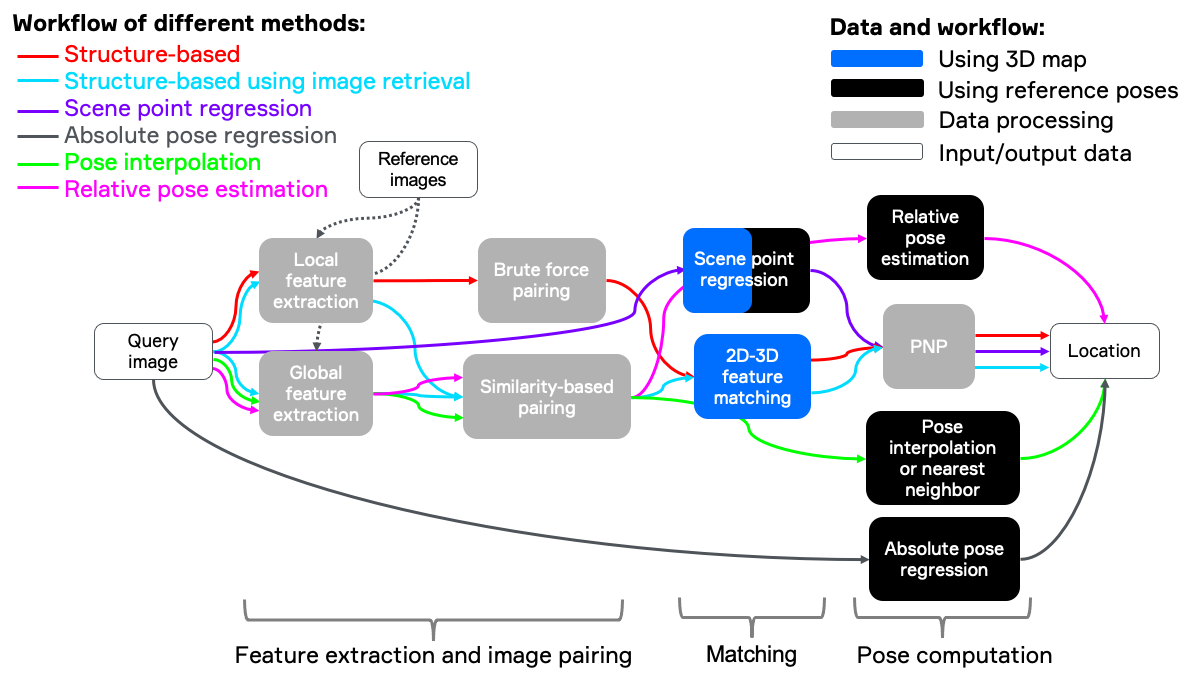
\includegraphics[scale=0.45]{pics/Chapter2/overviewViLoc.png}
    \caption{Tổng quát về những phương pháp bản địa hóa trực quan quan trọng \cite{methodsLocal}}
\end{figure}

\subsection{Những phương pháp sử dụng biểu diễn 3D}
\subsubsection*{Ý tưởng}
Những phương pháp sử dụng biểu diễn 3D sẽ hoạt động xoay quanh việc biểu diễn lại môi trường đang xét bằng một bản đồ đám mây điểm 3D. Bản đồ 3D chứa những đặc trưng trích xuất được từ các ảnh và tiến hành kiếm các cặp đặc trưng tương quan giữa các ảnh với nhau nhằm tạo thành những điểm mô tả 3D trong không gian ba chiều. Những bản đồ này thường sẽ được mô hình tạo ra vào lúc tiền xử lý tập dữ liệu và sẽ được dùng trong suốt quá trình bản địa hóa của mô hình.
\subsubsection*{Những bước thực hiện}
\begin{itemize}
    \item Ở bước tiền xử lý, không gian được thể hiện bởi tập dữ liệu sẽ được tái tạo lại trong không gian 3D, sử dụng những ảnh cùng thể hiện một cảnh, nhưng từ những vị trí và góc nhìn khác nhau. Phương pháp tái tạo này được gọi là Tái tạo kiến trúc từ chuyển động - Structure from Motion. Cụ thể hơn, quá trình này sẽ gồm các giai đoạn:
    \begin{itemize}
        \item Trích xuất mô tả của các đặc trưng từ ảnh: Mỗi ảnh trong tập dữ liệu sẽ được trích xuất đặc trưng và mỗi đặc trưng sẽ được gán một giá trị mô tả để SfM có thể tìm được những đặc trưng tương đồng giữa các hình. Kết quả đầu ra sẽ là một tập các mô tả cho đặc trưng của từng ảnh.
        \item Tìm kiếm sự tương quan của các đặc trưng giữa các ảnh: SfM sẽ tìm kiếm những ảnh cùng nhìn bộ phận của cảnh bằng cách kiểm tra sự tương đồng giữa các mô tả của đặc trưng trên các ảnh. Những cặp ảnh chứa những cặp đặc trưng tương quan sẽ cần được xác nhận lại về tính đúng đắn về hình học qua việc có tồn tại một cách biến đổi có khả năng ánh xạ một số lượng trưng giữa hai ảnh.
        \item Tái tạo lại cấu trúc: Quá trình tái tạo lại cấu trúc sẽ bắt đầu từ một cặp ảnh khởi tạo. Sau đó, góc nhìn
    \end{itemize}
\end{itemize}
\subsubsection*{Những biến thể của phương pháp}
\subsubsection*{Phân tích ưu và nhược điểm của phương pháp}

\subsection{Những phương pháp hồi quy vị trí}
\subsubsection*{Ý tưởng}
\subsubsection*{Những bước thực hiện}
\subsubsection*{Những biến thể của phương pháp}
\subsubsection*{Phân tích ưu và nhược điểm của phương pháp}

\subsection{Những phương pháp khác}
\subsection{Xác định những vấn đề hiện hữu trong bài toán bản địa hóa trực quan}

\begin{itemize}
    \item \textbf{Những phương pháp sử dụng biểu diễn 3D}
    \begin{itemize}
        \item Vấn đề về việc tiền xử lý: Để những phương pháp này có thể hoạt động được, một bản đồ điểm 3D thể hiện khu vực đang xét cần phải được tạo ra trước tiên. Bản đồ này có thể trở nên rất lớn khi mà khu vực đang xét đến là cả một tòa nhà, hay một thành phố.
        \item Vấn đề về lưu trữ: Trong quá trình hoạt động của mô hình, khi nhận vào một ảnh truy vấn, mô hình sẽ tiến hành việc tìm tương quan 2D-3D giữa các điểm trên hình và các điểm trên bản đồ 3D. Vì vậy nên, mô hình sẽ cần phải dành ra một lượng lớn tài nguyên bộ nhớ để lưu trữ bản đồ điểm 3D của khu vực đang xét.
        \item Vấn đề về khả năng khái quát hóa: Do mỗi bản đồ điểm 3D chỉ có thể phản ánh được một khu vực nhất định, hệ thống sẽ không thể xử lý được những ảnh truy vấn của những khu vực khác được. Trong trường hợp này, một tập ảnh mới của khu vực mới sẽ cần được thu thập để tạo thành một bản đồ điểm 3D mới.
    \end{itemize}
    %Để giải quyết những vấn đề trên, một phương pháp khác đã được đề xuất là xây dựng bản đồ điểm 3D cục bộ. Thay vì sinh ra bản đồ 3D cho toàn bộ khu vực đang xét ở bước tiền xử lý, phương pháp này sẽ sử dụng những ảnh truy xuất được để sinh ra bản đồ cục bộ \cite{sattler2017large}. Phương pháp này có thể tận dụng được những điểm mạnh của việc sử dụng cách biểu diễn 3D mà không cần duy trì bản đồ điểm 3D của toàn bộ khu vực. Tuy nhiên, cách tiếp cận này vẫn có một số điểm yếu như việc thời gian chạy trở nên đáng kể và số lượng ảnh truy xuất được có thể chưa đủ để sinh ra một bản đồ 3D phù hợp.

    Một cách tiếp cận khác với mục tiêu loại bỏ sự cần thiết của bản đồ 3D, sử dụng mạng học sâu để xác định được vị trí của một điểm ảnh trong môi trường 3D, gọi là hồi quy điểm trong cảnh - Scene Point Regression. Tuy nhiên, những mô hình thuộc phương pháp này không có tính khái quát hóa mà để có thể chạy trên một khu vực nhất định thì mô hình cần dữ liệu mẫu thuộc khu vực đó để huấn luyện.
    \item \textbf{Những phương pháp hồi quy vị trí}
    \begin{itemize}
        \item Vấn đề về phạm vi hoạt động của mô hình: Đa số những mô hình hồi quy vị trí đều chỉ hoạt động tốt trên những tập dữ liệu có phạm vi nhỏ và phân bố dày đặc như 7Scenes \cite{6619221} và Cambridge Landmarks \cite{kendall2016posenet}. Đối với những tập dữ liệu có phạm vi rộng và phân bố thưa như Aachen Day-Night \cite{Sattler2012ImageRF}, chỉ phương pháp nội suy đơn giản đã được áp dụng và kết quả đem lại là không quá tốt.
        \item Vấn đề về khả năng khái quát hóa: Những mô hình hồi quy tuyệt đối sẽ xây dựng ngầm biểu diễn của khu vực đang xét bên trong những trọng số của mô hình. Vì vậy nên, một mô hình được huấn luyện trên một không gian nhất định chỉ có thể xử lý những ảnh được chụp trong không gian đó. Đối với những mô hình hồi quy tương đối, vấn đề này sẽ phụ thuộc vào cơ chế truy xuất ảnh được sử dụng.
        \item Vấn đề về độ chính xác: Những phương pháp hồi quy sẽ không cho ra kết quả chính xác như những phương pháp sử dụng cách biểu diễn 3D.
    \end{itemize}
    \item \textbf{Những phương pháp truy xuất ảnh}
    \begin{itemize}
        \item Vấn đề về tài nguyên xử lý: Tuy bài toán VPR đã có nhiều bước đột phá trong thời gian qua, đa số các phương pháp đạt kết quả tốt đều sử dụng những cách tổng hợp mô tả của các đặc trưng trong ảnh như NetVLAD \cite{arandjelović2016netvlad} hoặc những biến thể tích hợp cơ chế tập trung \cite{keetha2023anyloc}, ngữ nghĩa của bộ phận ảnh \cite{peng2021semantic}, bối cảnh của ảnh \cite{jin2017learned}. Những cơ chế đó sẽ có ảnh hưởng tiêu cực đến thời gian chạy do độ phức tạp của giải thuật cũng như độ lớn của không gian mô tả.
        \item Vấn đề về khả năng biểu diễn của CNN: Những cách tiếp cận theo mô hình học sâu sử dụng CNN cho đến hiện tại thường sẽ gặp những vấn đề trong việc biểu diễn được những thông tin về môi trường địa lý trong bài toán bản địa hóa trực quan.
    \end{itemize}
\end{itemize}

\section{Nhận dạng địa điểm trực quan - Visual Place Recognition}

Trước đây, việc định vị trực quan trên quy mô lớn (large-scale visual localization) được coi là một vấn đề truy xuất hình ảnh\cite{2022arXiv220105816X}. Vị trí cho hình ảnh truy vấn được xác định bởi hình ảnh tương tự nhất được lấy từ cơ sở dữ liệu. Tuy nhiên, để đáp ứng nhu cầu xác định vị trí của ảnh với độ chính xác trên 6 bậc tự do (6 Degrees of Freedom), việc sử dụng mô hình 3D để ước tính tư thế của máy ảnh ngày càng được các nhà nghiên cứu đề xuất và sử dụng. Sử dụng phương pháp này, bài toán định vị trực quan có thể được chia thành hai bước: truy xuất hình ảnh và định vị tư thế máy ảnh từ hình ảnh truy xuất được.

\subsection{Học biểu diễn - Representational learning}

\subsection{Học biểu diễn NetVLAD}

\subsection{Tối ưu hóa đặc trưng - MAC}

\subsection{Trung bình Hölder - Trung bình GeM}

\subsection{Truy xuất và tái xếp hạng}

\subsection{Học biểu diễn bằng Vision Transformer}

\subsection{Học biểu diễn bằng Feature Mixer}

\section{Ước tính vị trí của máy ảnh - Pose Estimation}

Ước tính vị trí máy ảnh (Camera Pose Estimation) là một bài toán thuộc chuyên ngành thị giác máy tính nhằm xác định vị trí (position) và góc quay (orientation) chính xác nhất có thể của máy ảnh thông qua dữ liệu hình ảnh được chụp từ chính máy ảnh. Đây là một bước cực kỳ quan trọng trong việc giải quyết bài toán bản địa hóa trực quan, thường được áp dụng sau khi bước nhận dạng địa điểm trực quan đã trích xuất được ảnh từ kho dữ liệu. Hiện nay, có tương đối nhiều hướng tiếp cận đối với bài toán này. Một trong những phương pháp phổ biến nhất là huấn luyện một mô hình học sâu để xác định 6 chiều tự do (Degree of Freedom) từ số ít ảnh (Absoblute Pose Regression và Relative Pose Regression) hoặc xây dựng một mô hình 3D từ tập dữ liệu có sẵn rồi tiến hành chuyển ảnh đầu vào sang các điểm 3D để dễ dàng so sánh và xác định vị trí (Structure From Motion).

\subsection{Hồi quy vị trí tuyệt đối - Absolute Pose Regression}

Hồi quy vị trí tuyệt đối (Absolute Pose Regression) hướng đến việc dự đoán vị trí và góc quay chính xác nhất của ảnh bằng một mô hình mạng nơ-ron tích chập thông qua việc cải thiện trọng số của mô hình. Tùy thuộc vào đầu vào của mô hình mà hồi quy vị trí tuyệt đối được chia thành ba hướng chính: hồi quy vị trí tuyệt đối với một ảnh, chuỗi ảnh hoặc đoạn phim.

\subsubsection*{Hồi quy vị trí tuyệt đối đơn ảnh - Absolute pose regression through single monocular image}
Với phương pháp hồi quy vị trí tuyệt đối thông qua một ảnh (Absolute pose regression through single monocular image), quy trình chung thường bao gồm: đầu vào - mạng - đầu ra. Đầu vào sẽ là một ảnh RGB với đầu ra là vị trí 6 độ tự do của máy ảnh. Thông thường, kiến trúc của mạng lưới tính toán sẽ bao gồm các thành phần như sau: bộ mã hóa, bộ định vị, bộ hồi quy. 

\begin{figure}[H]
    \centering
    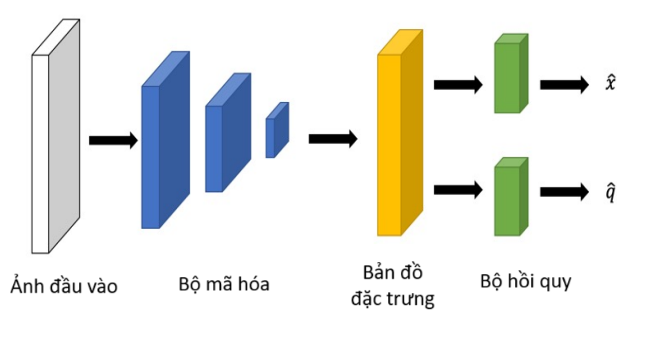
\includegraphics[scale=0.7]{pics/Chapter2/kientruc_APR_1.png}
    \caption{Kiến trúc mô hình hồi quy vị trí tuyệt đối đơn ảnh \cite{kendall2016posenet}}
\end{figure}

\noindent\textbf{Phương pháp sử dụng hàm mất mát Euclidean cố định:}

PoseNet \cite{kendall2016posenet} là công trình đầu tiên huấn luyện mô hình mạng nơ-ron tích chập để hồi quy vị trí máy ảnh từ một ảnh RGB, hoàn toàn không phụ thuộc vào bất kỳ cơ chế bên ngoài nào khác. Vào thời điểm ra mắt, PoseNet đã cho thấy sự vững chắc của mô hình vượt trội so với phương pháp tái tạo kiến trúc từ chuyển động dựa trên cơ chế "biến đổi tính năng bất biến tỷ lệ" (Scale-invariant Feature Transform Structure from Motion): độ hiệu quả của kiến trúc vế sau giảm mạnh nếu độ lớn của tập dữ liệu huấn luyện giảm đến một mức nhất định. Hàm mất mát Euclidean của PoseNet được định nghĩa như sau:
\begin{center}
$loss(I) = \left \| \hat{x} - x \right \|_2 + \beta \left \| \hat{q} - \frac{q}{\left \| q \right \|} \right \|_2$
\end{center}

Kế thừa từ PoseNet, đã có nhiều công trình và bài báo tìm cách cải thiện phương pháp định vị hoặc thay thế hàm mất mát nhằm nâng cao hiệu suất chung của toàn kiến trúc. Với các công trình có mong muốn cải thiện hàm mất mát của mô hình, một chiến thuật chung là kết hợp hàm mất mát Euclidean và phương pháp giảm độ dốc Stochastic. Về mặt cải thiện hiệu quả định vị cũng như tìm hiểu về độ thiếu chính xác của mô hình, một nhóm tác giả đề xuất thêm xác suất Bernoulli vào mô hình nơ-ron tích chập \cite{kendall2016modelling} nhằm xác định độ thiếu chính xác của mô hình. Ý tưởng chính của phương pháp này là xác định và tận dụng độ thiếu chính xác để dự đoán sai số trong định vị, phương pháp này đã cải thiện độ chính xác cho PoseNet cho cả những cảnh ngoài trời và bên trong nhà.
\begin{figure}[H]
    \centering
    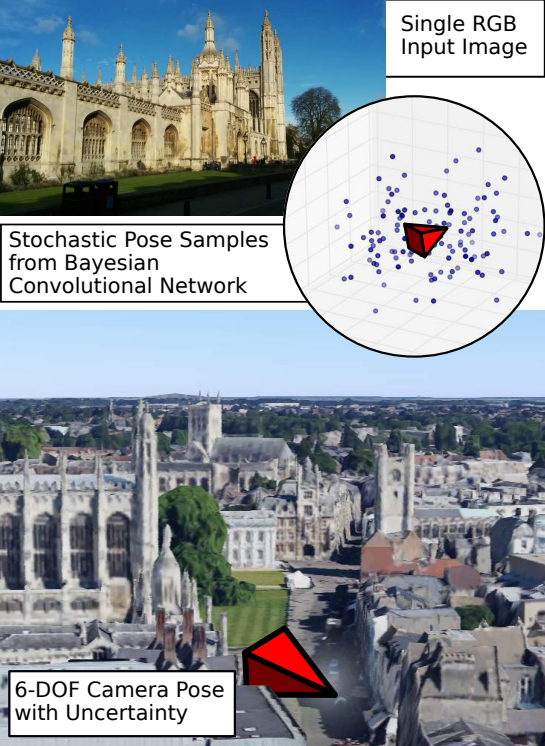
\includegraphics[scale=0.7]{pics/Chapter2/Ber_PoseNet.png}
    \caption{Minh họa mô hình CNN được áp dụng phân phối Bernoulli \cite{kendall2016modelling}}
\end{figure}
Từ những thông tin được nêu ra trong bài báo \cite{kendall2016posenet}, ta biết được rằng mô hình PoseNet có một lớp kết nối đầy đủ với 2048 chiều, tạo điều kiện cho việc áp dụng một lớp bộ nhớ dài ngắn hạn để giảm chiều đặc trưng giúp cải thiện độ chính xác định vị \cite{walch2017imagebased, wang2019atloc}. Nhóm tác giả Watch và cộng sự \cite{walch2017imagebased} đề xuất tận dụng các lớp bộ nhớ dài ngắn hạn lên đầu ra của PoseNet để giảm chiều và chọn ra những đặc trưng hữu ích nhất cho bài toán định vị vị trí. Các thí nghiệm đo lường cho thấy phương pháp này vượt trội hơn PoseNet khoảng 30\% về sai số vị trí và 55\% về sai lệch góc quay.
\begin{figure}[H]
    \centering
    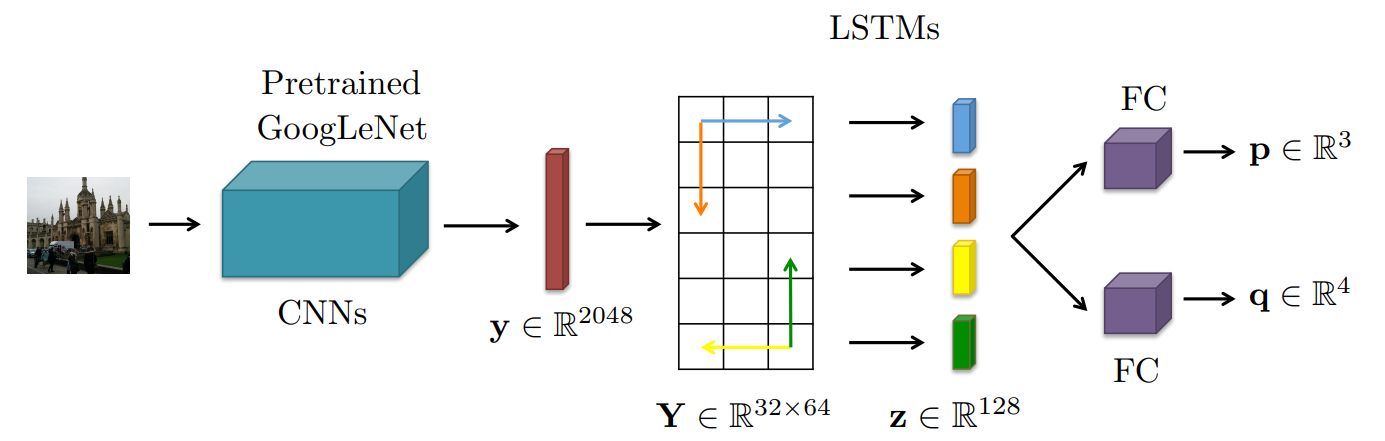
\includegraphics[width=\textwidth]{pics/Chapter2/LSTM_PoseNet.png}
    \caption{Minh họa kiến trúc mô hình LSTM PoseNet \cite{walch2017imagebased}}
\end{figure}
Để cải thiện độ chính xác định vị, một kiến trúc đồng hồ cát được đề xuất với việc thêm một phần chức năng mã hóa thông tin hữu ích từ kiến trúc vật thể thô và một phần chức năng thu chi tiết vật thể mịn. Hourglass PoseNet \cite{melekhov2017imagebased} có kiến trúc gồm ba thành phần chính là bộ mã hóa, bộ giải mã và bộ hồi quy. Mô hình này sử dụng một mô hình ResNet34 đã được tinh chỉnh làm bộ mã hóa - giải mã. SVS PoseNet \cite{inproceedings} dùng mô hình VGG16 kết hợp thêm hai lớp kết nối đầy đủ để có thể dự đoán riêng vị trí và góc quay. BranchNet \cite{7989663} sử dụng mô hình mạng hai nhánh học đồng thời biểu diễn góc quay và độ dời để giảm thiểu độ thưa của các vị trí được lấy mẫu một cách hiệu quả. Dù hướng tiếp cận có sự khác biệt, các công trình trên đều có cùng hàm mất mát với PoseNet.
\begin{figure}[H]
    \centering
    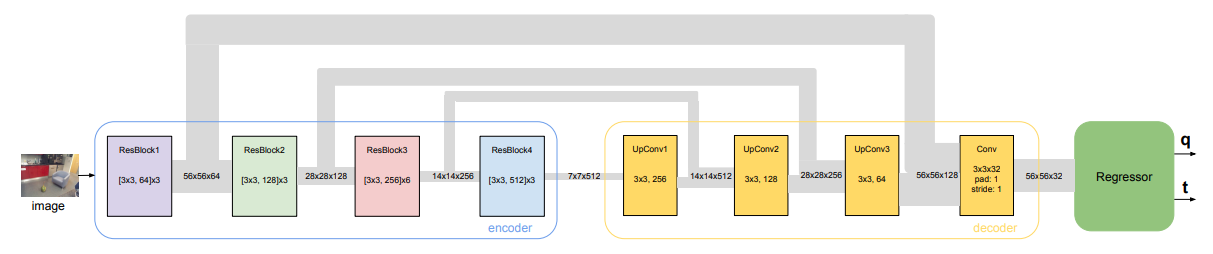
\includegraphics[width=\textwidth]{pics/Chapter2/hourglass_PoseNet.png}
    \caption{Minh họa kiến trúc mô hình Hourglass PoseNet \cite{melekhov2017imagebased}}
\end{figure}

\noindent\textbf{Phương pháp sử dụng hàm mất mát có trọng số học được:}

Để học được thông tin về vị trí và góc quay từ dữ liệu ảnh, hàm mất mát cố định Euclidean áp dụng các siêu tham số cân bằng để giúp việc học thông tin vị trí và góc quay một cách độc lập, tuy nhiên để học trọng số thì rất tốn kém. Geometric PoseNet \cite{kendall2017geometric} đề xuất sử dụng hàm mất mát vị trí có trọng số học được để cân bằng hiệu suất và cải thiện độ ổn định. Khi so sánh với PoseNet, phương pháp này giữ lại độ mở rộng và độ chắc chắn mà không cần chỉnh sửa các siêu tham số cố định cân bằng trong hàm mất mát. 

AtLoc \cite{wang2019atloc} thêm vào mô hình một mô-đun tập trung (Attention Module) trước khi xác định các tọa độ hồi quy để ép buộc mạng phải tập trung vào phần chính - phần mang nhiều thông tin hữu ích nhất của hình ảnh đầu vào. Ngoài ra, AtLoc sử dụng ResNet34 được huấn luyện sẵn trên tập dữ liệu ImageNet làm bộ mã hóa, sau đó hồi quy lớp kết nối đầy đủ 2048 chiều của PoseNet. 
\begin{figure}[H]
    \centering
    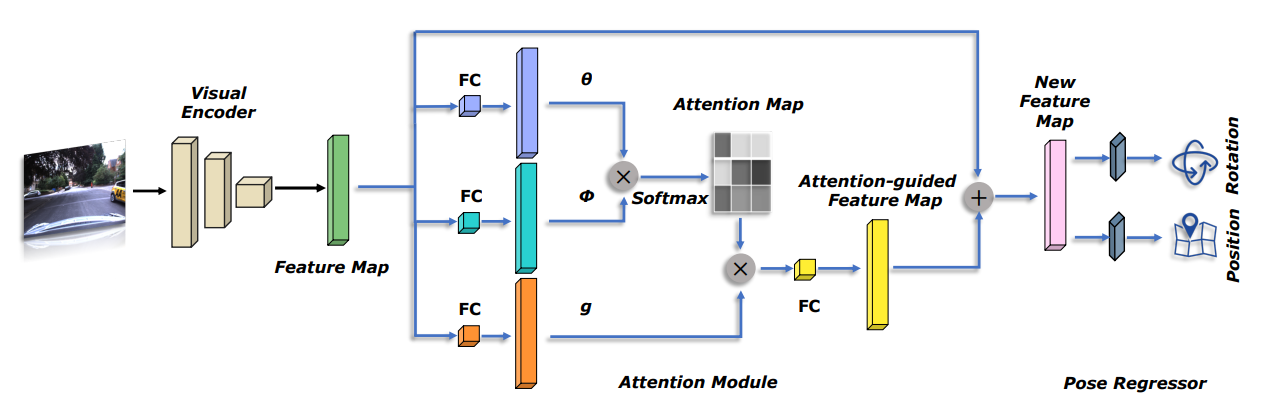
\includegraphics[width=\textwidth]{pics/Chapter2/atloc.png}
    \caption{Minh họa kiến trúc mô hình AtLoc \cite{wang2019atloc}}
\end{figure}
AdPR \cite{bui2019adversarial} thêm một mạng phân biệt và học đối lập. Điều này không chỉ hồi quy vị trí mà còn tinh chỉnh vị trí. Khi trích xuất đặc trưng, AdPR áp dụng mạng ResNet-18, vì nó có thể đạt được hiệu suất tốt nhất so với VGG16 và AlexNet. APANet \cite{chidlovskii2020adversarial} cũng sử dụng một mạng đối lập để tạo ra hình ảnh liên quan đến hình ảnh đầu vào để ước lượng tốt hơn vị trí của máy ảnh. Một mô-đun Dropout được thêm trước bộ mã hóa trích xuất đặc trưng để xuất ra nhiều khả năng không chắc chắn, điều này có thể cải thiện độ chắc chắn của mô hình dưới điều kiện thử thách như thay đổi vị trí, thời tiết,... . Sau khi trích xuất, mô-đun tập trung tự động được thêm để điều chỉnh lại trọng số bản đồ đặc trưng.
\begin{figure}[H]
    \centering
    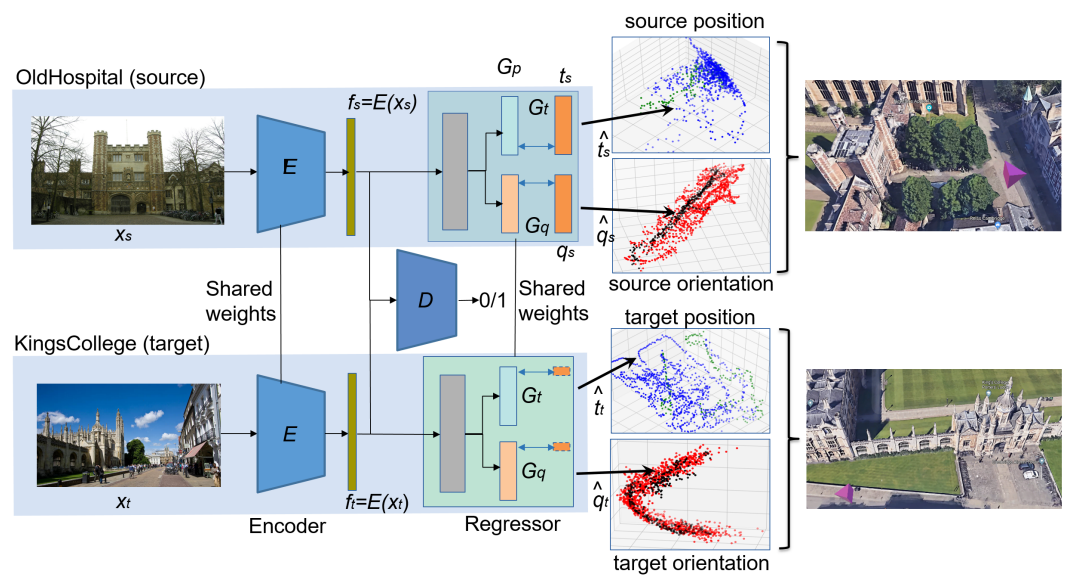
\includegraphics[width=\textwidth]{pics/Chapter2/apanet.png}
    \caption{Minh họa kiến trúc mô hình APANet \cite{chidlovskii2020adversarial}}
\end{figure}
\noindent\textbf{Phương pháp sử dụng hàm mất mát khác:}

Không dùng đến cả hàm mất mát cố định hoặc những hàm mất mát có trọng số học được, một số nhóm nghiên cứu đề xuất nên cân nhắc sử dụng các mô-đun khác để cải thiện hiệu suất định vị. GeoPoseNet \cite{kendall2017geometric} đề xuất sử dụng hàm mất mát tái chiếu: đặc tả sai sót tái chiếu của cảnh. Hàm mất mát tái chiếu chuyển mất mát chung học được thành khác biệt tọa độ ảnh, do đó có thể thay đổi trọng số giữa vị trí và góc quay, tùy thuộc vào các cảnh khác nhau trong quá trình huấn luyện mô hình. GPoseNet \cite{Cai2018AHP} xây dựng mô hình mới bằng cách thêm vào hai bộ "Hồi quy quá trình Gaussian suy luận biến phân ngẫu nhiên" (Stochastic Variational Inference Gaussian Process Regressions - SVI GPs) sau lớp kết nối đầy đủ để học phân phối xác suất của vị trí - hướng quay đầu ra và giảm tần suất sử dụng siêu tham số. Hàm mất mát của GPoseNet kết hợp hàm mất mát SVI GPs sử dụng ranh giới điều kiện dưới của hai xác suất tích lũy log $L_{s}vi$ và hàm mất mát CNN với siêu tham số $\beta_{g_{t}}$ và $\beta_{n_{q}}$ của PoseNet.
\begin{figure}[H]
    \centering
    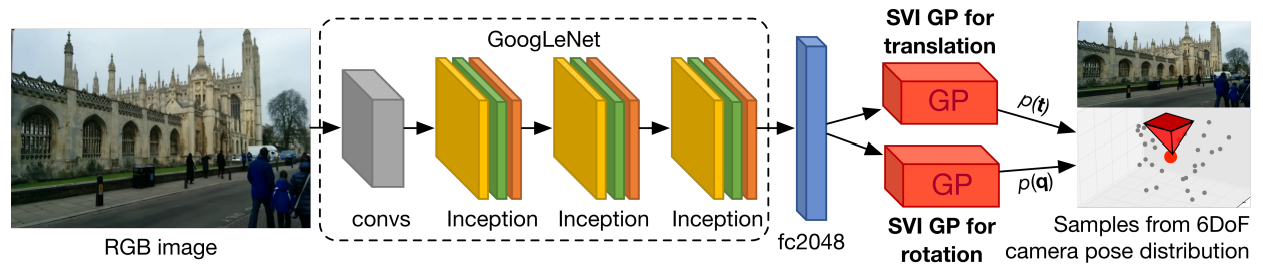
\includegraphics[width=\textwidth]{pics/Chapter2/gposenet.png}
    \caption{Minh họa kiến trúc mô hình GPoseNet \cite{kendall2017geometric}}
\end{figure}

Một nhóm nghiên cứu \cite{shavit2021learning, article} đề xuất áp dụng mô hình Transformer vào tác vụ hồi quy vị trí tuyệt đối. Mô hình nhận vào một ảnh đơn và sử dụng một CNN làm bộ trích xuất đặc trưng, sau đó các bản đồ đặc trưng được truyền song song qua hai nhánh: mỗi nhánh là một mô hình Transformer đảm nhiệm một tác vụ riêng lần lượt là hồi quy vị trí và hồi quy hướng quay. Mô hình sử dụng hàm mất mát tương tự với PoseNet.
\begin{figure}[H]
    \centering
    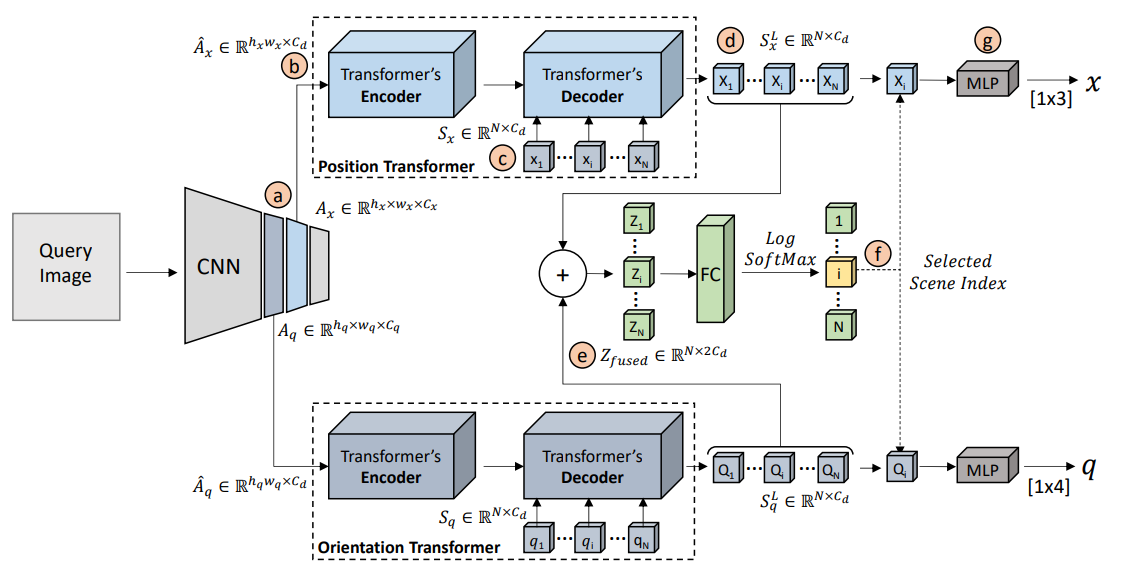
\includegraphics[width=0.7\textwidth]{pics/Chapter2/trans.png}
    \caption{Minh họa kiến trúc mô hình Multi-Scene Transformer \cite{shavit2021learning, article}}
\end{figure}

\subsubsection*{Hồi quy vị trí tuyệt đối đa ảnh - Absolute pose regression through auxiliary image sequence}
Một phương pháp khác được áp dụng để hồi quy vị trí tuyệt đối là áp dụng học có hỗ trợ với một chuỗi ảnh. Học có hỗ trợ được định nghĩa là phương pháp cải thiện hiệu suất của một tác vụ chính thông qua việc học cùng lúc các tác vụ hỗ trợ. Phương pháp học này giúp mô hình phát triển các biểu diễn dữ liệu tốt hơn. Bằng cách tận dụng các tác vụ hỗ trợ có liên quan khác trong quá trình học, hiệu suất của tác vụ chính có thể được cải thiện. Ở đây, học có hỗ trợ ám chỉ việc kết hợp APR với các tác vụ phụ có liên quan như đo lường cảm biến trực quan. Hàm mất mát của các phương pháp học có hỗ trợ thường bao gồm hàm mất mát của APR kết hợp với hàm mất mát của các phương pháp phụ trợ, thậm chí có thể kết hợp cả hàm mất mát của APR và RPR. Khác với các phương pháp hồi quy vị trí tuyệt đối đơn ảnh, phương pháp học có hỗ trợ học từ các cặp ảnh với bản chất là học cách xác định vị trí tuyệt đối bằng cách đánh giá trước hết vị trí tương đối với các ràng buộc phụ thuộc.

MapNet \cite{brahmbhatt2018geometryaware} đề xuất thêm một thuật ngữ mất mát lấy từ các cặp ảnh làm một ràng buộc hình học, điều này đã có thể cải thiện mạnh mẽ hiệu suất khả năng định vị. Về hàm mất mát, MapNet giảm thiểu tối đa cả mất mát vị trí tuyệt đối cho mỗi hình ảnh và mất mát vị trí tương đối giữa các cặp hình ảnh:
\begin{center}
    $l(I_{total}) = l(I_i) + \alpha\sum_{i\neq j}loss(I_{ij} )$
\end{center}
Trong đó, $loss(I_{ij} )$ ám chỉ vị trí máy ảnh tương đối $p_i$ và $p_j$ giữa các cặp hình ảnh $I_i$ và $I_j$, được tính bởi hàm mất mát với trọng số có thể học được.

Thêm vào đó, MapNet chuyển một giá trị quaternion thành logarit của giá trị đó - biểu diễn phép quay ba độ tự do (3DoF) với ba chiều chưa bị tham số hóa quá mức. $logq$ được biểu diễn như dưới đây, với $u$ và $v$ đại diện cho phần thực và ảo của một quaternion đơn vị:
\begin{center}
    $logq = 
    \begin{cases}
      \frac{v}{\left \| v \right \|}cos^{-1}u, \left \| v \right \| \neq 0\\    
      0   
    \end{cases}$
\end{center}
\begin{figure}[H]
    \centering
    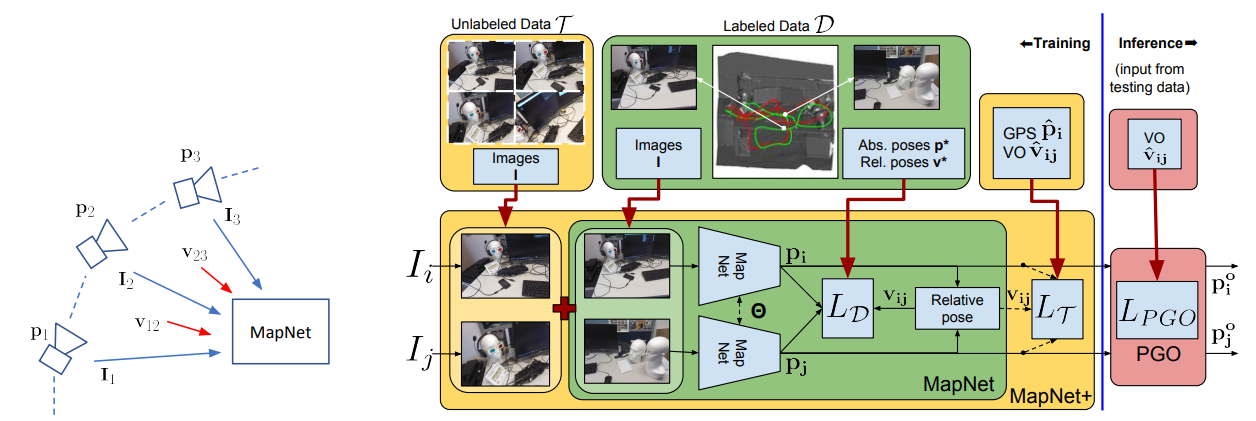
\includegraphics[width=\textwidth]{pics/Chapter2/mapnet.png}
    \caption{Minh họa kiến trúc mô hình MapNet \cite{brahmbhatt2018geometryaware}}
\end{figure}
Năm 2019, tác giả Xue và những cộng sự \cite{xue2019local} cũng có một hướng tiếp cận tương tự khi hồi quy vị trí máy ảnh thông qua những ràng buộc về không gian - thời gian, trong đó đặc trưng cục bộ cải thiện định vị toàn cục - gọi là "Cục bộ hỗ trợ toàn cục" (Local Support Global - LSG). Thêm vào đó, LSG đề xuất sử dụng một đánh giá đã được “tăng cường nội dung” để ước lượng lỗi vị trí và tinh chỉnh dựa trên chuyển động, để tối ưu hóa dự đoán vị trí thông qua các ràng buộc chuyển động. LSG sử dụng một hàm mất mát vị trí toàn cầu $L_g$ lấy từ hồi quy tuyệt đối, hàm mất mát hồi quy đo lường cảm biến trực quan $L_{vo}$, các ràng buộc hình học và hàm mất mát liên kết chuyển động $L_{joint}$ để tối ưu hóa hồi quy vị trí như sau:
\begin{center}
$l_{total} = l_g + l_{vo} + l_{joint}$
\end{center}
\begin{figure}[H]
    \centering
    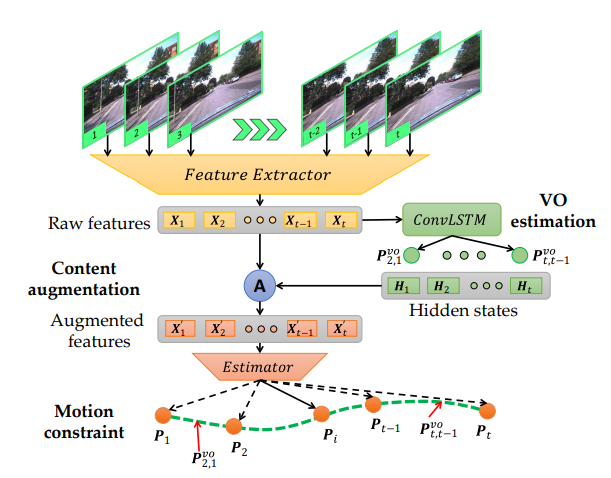
\includegraphics[width=0.5\textwidth]{pics/Chapter2/lsg.png}
    \caption{Minh họa kiến trúc mô hình LSG \cite{xue2019local}}
\end{figure}
VlocNet \cite{valada2018deep} cũng học đồng thời đo lường cảm biến trực quan như một tác vụ phụ để hồi quy vị trí toàn cục với hai mạng phụ. Mất mát nhất quán hình học được điều chỉnh để giảm thiểu tối đa lỗi vị trí, được định nghĩa như sau:
\begin{center}
$l(I_{total}) = (I_{i_x} + I_{ij_x})exp(-\hat{s}_x) + (I_{i_q} + I^{q}_{ij})exp(-\hat{s}_q)+ \hat{s}_q$
\end{center}
\begin{figure}[H]
    \centering
    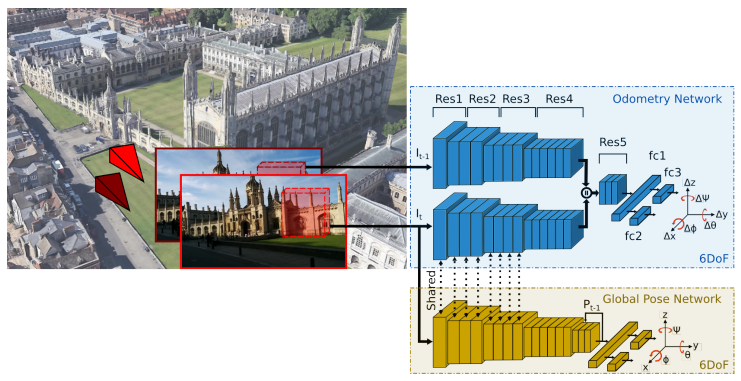
\includegraphics[width=0.7\textwidth]{pics/Chapter2/vlocnet.png}
    \caption{Minh họa kiến trúc mô hình VlocNet \cite{valada2018deep}}
\end{figure}
VlocNet++ \cite{Radwan_2018} giới thiệu kiến thức ngữ nghĩa vào hồi quy vị trí, kết hợp thông tin hình học-thời gian với các đặc trưng ngữ nghĩa cùng một lúc. Hàm mất mát của VlocNet++ kết hợp hồi quy vị trí toàn cục, mất mát đo lường cảm biến trực quan và mất mát Entropy chéo cho mất mát phân đoạn ngữ nghĩa cùng một lúc, với ba yếu tố $\hat{s}_{log}$, $\hat{s}_{vo}$ và $\hat{s}_{seg}$ để cân bằng ba thành phần này:
\begin{center}
$ l(I_{total}) = l_{loc}exp(-\hat{s}_{loc})+ \hat{s}_{loc}+l_{vo}exp(-\hat{s}_{vo})+ \hat{s}_{vo}+l_{seg}exp(-\hat{s}_{seg})+ \hat{s}_{seg}$
\end{center}
\begin{figure}[H]
    \centering
    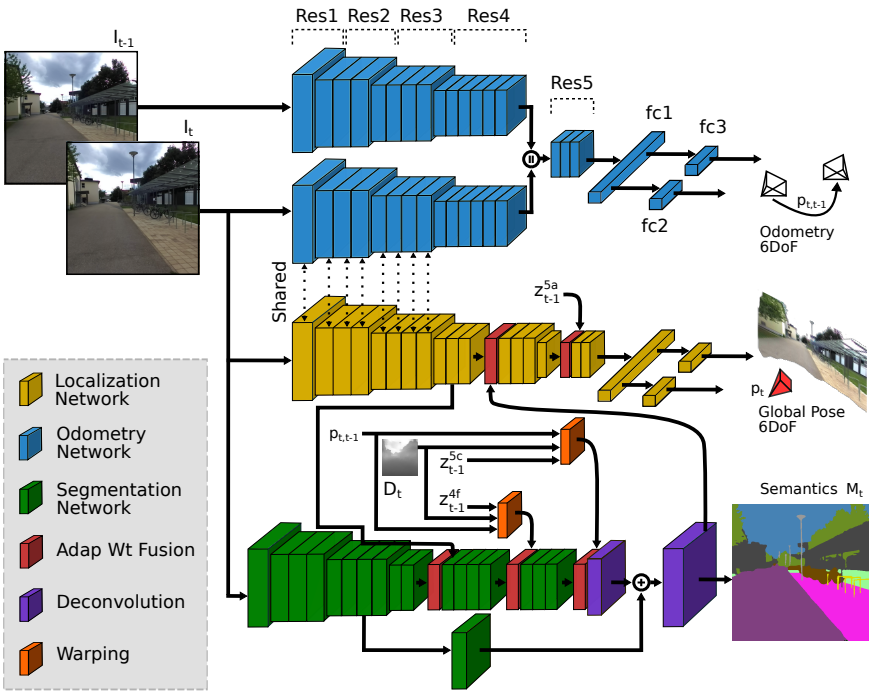
\includegraphics[width=0.7\textwidth]{pics/Chapter2/vlocnetplus.png}
    \caption{Minh họa kiến trúc mô hình VlocNet++ \cite{Radwan_2018}}
\end{figure}
Một bản mở rộng của AtLoc, AtLocPlus \cite{wang2019atloc} cũng kết hợp các ràng buộc thời gian để học cùng lúc mất mát vị trí tuyệt đối và mất mát vị trí tương đối, dẫn đến hiệu suất tốt hơn AtLoc trong việc sử dụng một đầu vào ảnh đơn. AtLocPlus sử dụng hàm mất mát giống với MapNet.

DGRNet \cite{lin2019deep} đề xuất một kiến trúc với một mạng con hồi quy vị trí tương đối RCNN1, một mạng con hồi quy vị trí toàn cục RCNN2 và lớp kết hợp kết nối đầy đủ dùng để trích xuất đặc trưng từ ảnh. Ràng buộc biến đổi chéo (Cross transformation constraint – CTC) và sai số toàn phương trung bình (Mean squared error – MSE) được áp dụng vào hàm mất mát để cải thiện hiệu suất hồi quy. DGRNet đã sử dụng kết hợp hàm mất mát tương đối, toàn cục, CTC $\hat{l}_i$ và sự thật nền tảng $\hat{P}_i$ như sau:
\begin{center}
$ w = \underset{w}{argmin} \frac{1}{N}^{N}_{i=1} \sum_{k=0}^{6}(l^i_k) + \sum_{j=0}^{4}\left \| P^ij - \hat{P}^i_j \right \|^2_2 $
\end{center}
\begin{figure}[H]
    \centering
    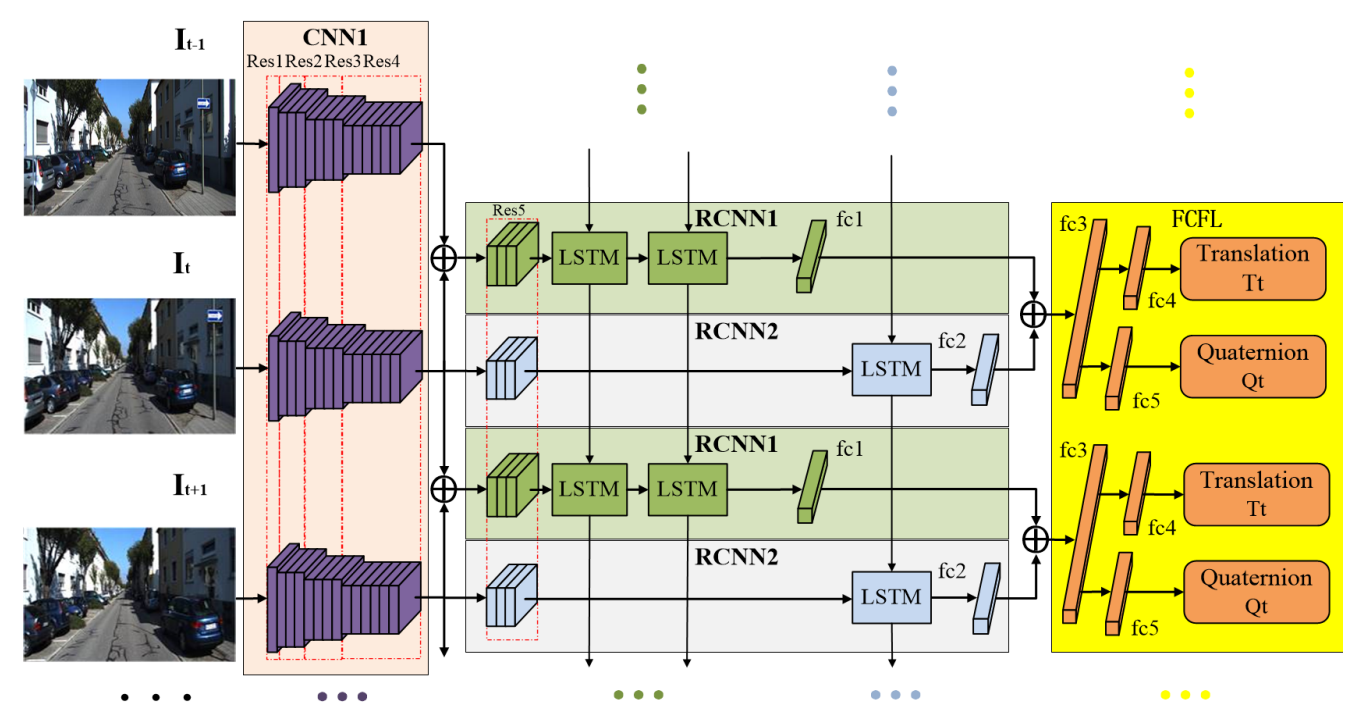
\includegraphics[width=0.7\textwidth]{pics/Chapter2/dgrnet.png}
    \caption{Minh họa kiến trúc mô hình DGRNet \cite{lin2019deep}}
\end{figure}
\subsubsection*{Hồi quy vị trí tuyệt đối qua đoạn phim - Absolute pose regression through video}

Không chỉ đơn ảnh hay đa ảnh, ngay cả đoạn phim cũng có thể được sử dụng để thêm một ràng buộc thời gian có tính trơn tru hơn cho hồi quy vị trí. Các đoạn phim hay các dữ liệu cảm biến khác đều có thể được truy cập dễ dàng bởi các thiết bị di động. Đoạn phim có thể được đồng bộ hóa với các dữ liệu đầu vào khác như đo lường cảm biến trực quan, các cảm biến IMU như đồng hồ tăng tốc và đồng hồ quay và dữ liệu GNSS bằng thông tin thời gian , cụ thể là bằng cách căn chỉnh các mốc thời gian. Với một quy trình tương tự như các phương pháp ARP dựa trên hình ảnh đơn và chuỗi hình ảnh, ARP dựa trên đoạn phim cũng hồi quy độ dời và hướng quay thông qua bộ trích xuất đặc trưng là một mạng nơ-ron tích chập và bộ hồi quy vị trí cục bộ.

VidLoc \cite{clark2017vidloc} đề xuất một mô hình hồi quy vị trí máy ảnh dựa trên việc kết hợp CNN – RNN, mục đích là có thể khiến quá trình dự đoán vị trí từ ảnh hay một đoạn phim được trơn tru hơn. Mạng được xây dựng bằng cách sử dụng GoogLeNet Inception \cite{szegedy2014going} mà không dùng đến lớp kết nối đầy đủ để trích xuất đặc trưng ảnh và một mô-đun LSTM hai chiều để mô hình hóa thông tin thời gian với các ô nhớ.  Hàm mất mát của VidLoc được tính bằng tổng của lỗi vị trí và lỗi hướng quay từ đầu ra của LSTM như sau:
\begin{center}
$ l = \sum_{t=1}^T \alpha_1 \left \| x_t - \hat{x}_t \right \| + \alpha_2 \left \| q_t - \hat{q}_t \right \| $
\end{center}
Với $[x_t, q_t]$ và $[\hat{x}_t, \hat{q}_t]$ đại diện cho sự thật nền tảng và giá trị dự đoán cho độ dời vị trí và hướng quay.
\begin{figure}[H]
    \centering
    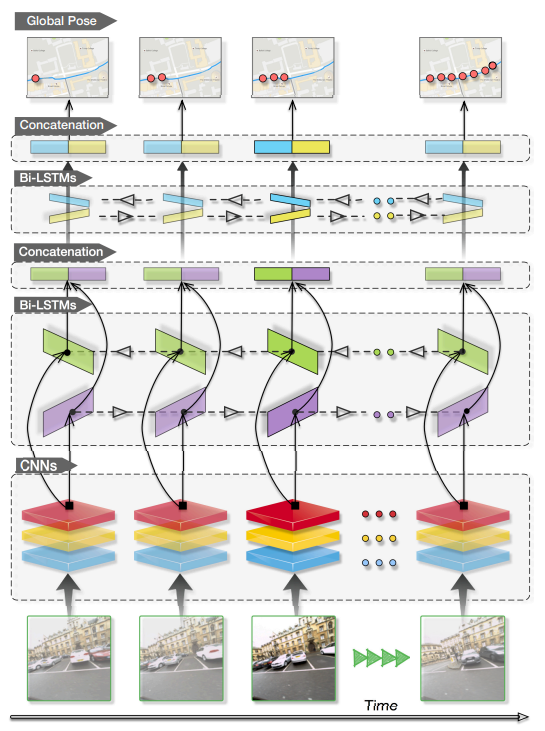
\includegraphics[width=0.7\textwidth]{pics/Chapter2/vidloc.png}
    \caption{Minh họa kiến trúc mô hình VidLoc \cite{clark2017vidloc}}
\end{figure}
MapNet+ và MapNet+PGO \cite{brahmbhatt2018geometryaware} mang cùng một kiến trúc mạng với MapNet trích xuất đặc trưng qua mạng ResNet34 và dùng một lớp tổng hợp trung bình toàn cục. Không chỉ dùng mất mát vị trí tuyệt đối, mất mát đo lường cảm biến trực quan cũng được tính toán để cải thiện hiệu suất dự đoán vị trí của MapNet. Phương pháp này cũng đồng thời tích hợp dữ liệu GNSS và IMU để giúp cải thiện hồi quy vị trí. Điều này giúp kết hợp dữ liệu đã được gắn nhãn và dữ liệu chưa gắn nhãn từ VO hay cảm biến để phục vụ cho việc học tự giám sát và đã thể hiện hiệu suất tốt dưới những điều kiện khó khăn, thử thách như thay đổi môi trường ngoài, thiếu sáng,... .
\begin{center}
$l = l_{labelled data} + l_{unlabelled data}$
\end{center}
Với mất mát từ dữ liệu chưa gắn nhãn có thể được tính toán thông qua việc kết hợp vị trí máy ảnh tương đối $v_ij$ và VO $\hat{v}_ij$ hay các cảm biến khác như IMU và GNSS. 

MapNet+PGO đã có thể cải thiện hiệu suất đồng thời giảm thiểu chi phí tính toàn thông qua việc sử dụng cải thiện đồ thị vị trí (PGO) để kết hợp kết quả vị trí MapNet+ và VO.

\subsubsection*{Kết luận}
Xét về các phương pháp mang hướng hồi quy vị trí tuyệt đối thông qua một ảnh duy nhất, các nghiên cứu có xu hướng tiến tới việc hàm mất mát tự động hóa, không sử dụng siêu tham số và mang nhiều thông tin hơn để giảm việc sử dụng các tham số cố định. Khởi đầu từ PoseNet với việc sử dụng một hàm mất mát cố định để tính tổng độ dời và hướng quay sử dụng một số tham số cân bằng. Sau đó, một hàm mất mát có trọng số học được \cite{wang2019atloc, bui2019adversarial} đã được đề xuất bằng cách thêm độ không đảm bảo phương sai đồng nhất để tự động cân bằng mất mát độ dời và hướng quay, tránh sử dụng siêu tham số đồng thời vượt qua hiệu suất của phương pháp sử dụng hàm mất mát cố định. Ngoài phương pháp hàm mất mát cố định và hàm mất mát với trọng số học được, một số công trình \cite{kendall2017geometric, Cai2018AHP} đề xuất sử dụng mất mát lỗi tái chiếu và mất mát GPoseNet để thêm các định dạng thông tin khác như phân phối xác suất của vị trí - hướng quay đầu ra để cải thiện hàm mất mát. 

Với việc sử dụng nhiều ảnh cũng như học kết hợp các tác vụ phụ, các mô hình đã có thể không chỉ thu được kết quả định vị mà còn có được thông tin khác như VO, thông tin ngữ nghĩa,etc. MapNet, VlocNet, AtLocPlus \cite{wang2019atloc} kết hợp cả hàm mất mát vị trí tương đối và vị trí tuyệt đối để cải thiện hiệu quả tác vụ hồi quy. LSG \cite{xue2019local} áp dụng một ràng buộc chuyển động vào hàm mất mát trong khi đó VlocNet++ \cite{Radwan_2018} thì đề xuất thêm ràng buộc ngữ nghĩa vào. DGRNet \cite{lin2019deep} kết hợp CTC và MSE vào quá trình tính toán hàm mất mát.

Cho rằng các phương pháp hồi quy vị trí tuyệt đối thông qua ảnh đang bỏ phí giá trị của các ràng buộc thời gian, một số công trình \cite{clark2017vidloc, brahmbhatt2018geometryaware} đề xuất việc tận dụng các đoạn phim làm đầu vào cho tác vụ hồi quy vị trí. VidLoc \cite{clark2017vidloc} sử dụng RNN hai chiều để hồi quy vị trí 6DoF của máy ảnh. MapNet+ và MapNet+PGO \cite{brahmbhatt2018geometryaware} chủ yếu tận dụng VO vào hàm mất mát để tăng cường hiệu quả tác vụ hồi quy.

\subsection{Hồi quy vị trí tương đối - Relative Pose Regression}

Mô hình hồi quy vị trí tuyệt đối học cách ánh xạ các pixel của ảnh sang vị trí của máy ảnh, thường được quyết định bởi hệ trục tọa độ của chính cảnh vật cụ thể mà máy ảnh đang chụp. Khác với hồi quy vị trí tuyệt đối, các phương pháp mang hướng tiếp cận hồi quy vị trí tương đối (Relative Pose Regression) chỉ tính toán vị trí tương đối của ảnh và thường được huấn luyện trên những tập dữ liệu đa cảnh để tăng cường khả năng mở rộng mô hình đầu cuối.

\subsubsection*{Hồi quy vị trí tương đối thông qua truy xuất rõ ràng - Relative camera pose regression through explicit retrieval}
Quy trình hồi quy vị trí tương đối của máy ảnh có thể được hiểu như một quy trình bao gồm truy xuất ảnh có độ tương đồng cao nhất trong kho dữ liệu với ảnh nhận đầu vào và sau đó dự đoán vị trí tương đối giữa chúng để lấy được vị trí tuyệt đối của ảnh nhận đầu vào. Cho một ảnh $I_a^c$ được chụp từ máy ảnh $c$, thông qua các phương pháp truy xuất ảnh từ kho dữ liệu, chúng ta có được ảnh có độ tương đồng cao nhất $I_b^c$. Nếu có được vị trí nền tảng $p_b$ của ảnh $I_b^c$ và vị trí tương đối giữa hai ảnh là $p_{a->b}$, vị trí tuyệt đối $p_a$ của ảnh đầu vào $I_a^c$ có thể được xác định bằng các phép biến đổi toán học.

NNnet \cite{laskar2017camera} là công trình đầu tiên đề xuất một phương pháp hồi quy vị trí tương đối dựa trên truy xuất ảnh. Đầu vào của phương pháp này là một ảnh và một kho dữ liệu ảnh có bao gồm vị trí nền tảng. Một tập các cặp ảnh được tận dụng để hồi quy vị trí tương đối thông qua một mạng Siamese với hai nhánh ResNet34 đã được hiệu chỉnh và một hàm mất mát cố định. Ảnh có độ tương đồng gần nhất với ảnh nhận đầu vào có thể được tính toán xác định thông qua bộ trích xuất đặc trưng hình thành bởi nhánh mạng CNN, sau đó vị trí tương đối và vị trí nền tảng của ảnh trích xuất sẽ kết hợp để tính toán xác định vị trí tuyệt đối của ảnh đầu vào.
\begin{figure}[H]
    \centering
    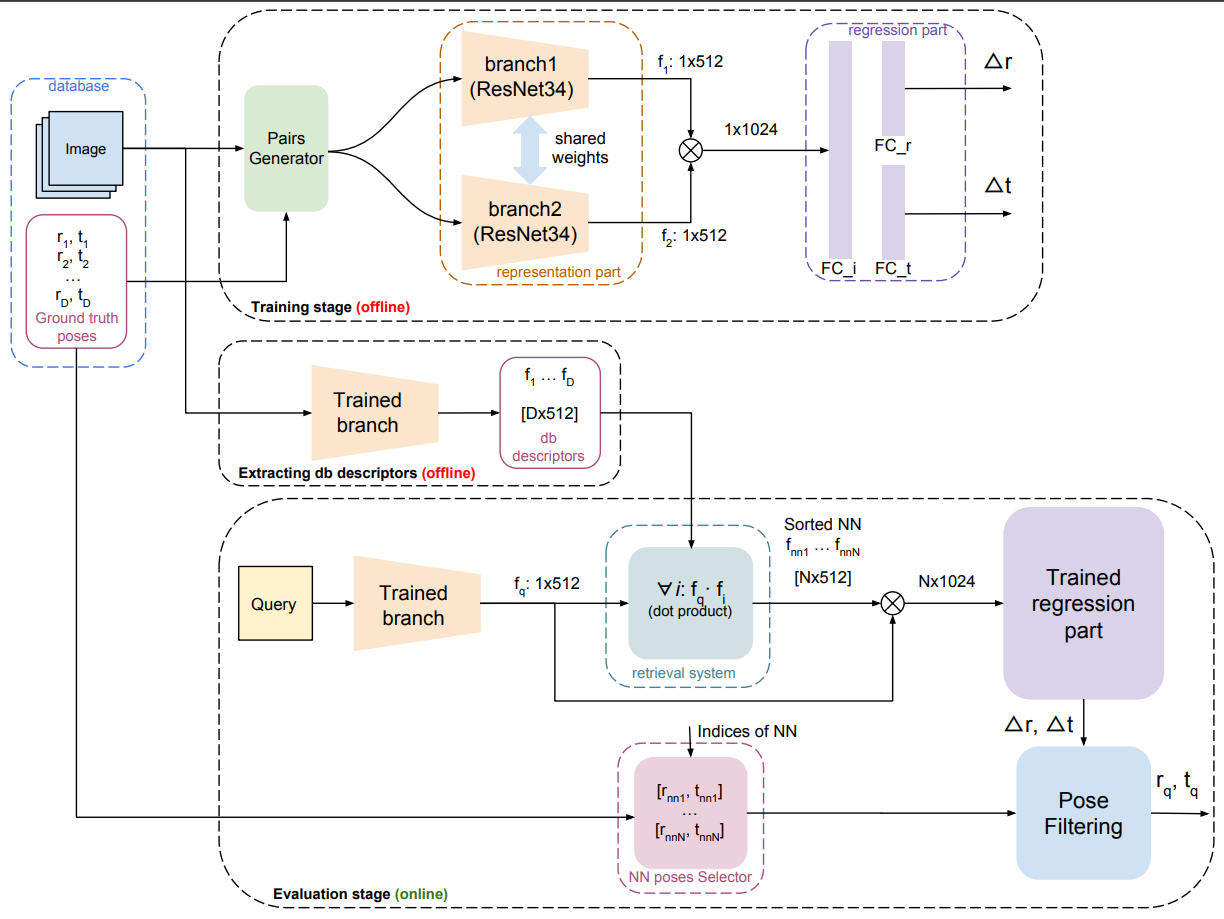
\includegraphics[width=0.7\textwidth]{pics/Chapter2/nnet.png}
    \caption{Minh họa kiến trúc mô hình NNet \cite{laskar2017camera}}
\end{figure}
RelocNet \cite{10.1007/978-3-030-01264-9_46} cải tiến NNet với việc học liên tục thước đo với mục đích học các đặc trưng ảnh toàn cục với một góc nhìn chóp cụt của máy ảnh để cải thiện kết quả, mất mát vị trí tương đối cũng được áp dụng. Mất mát vị trí tương đối học sự khác biệt vị trí giữa hai ma trận vị trí bằng cách sử dụng một biểu diễn ma trận cho hướng quay và độ dời vị trí. Hàm mất mát huấn luyện được định nghĩa như sau:
\begin{center}
$l = \alpha l_{SE(3)} + \beta l_{frustum}$
\end{center}
\begin{figure}[H]
    \centering
    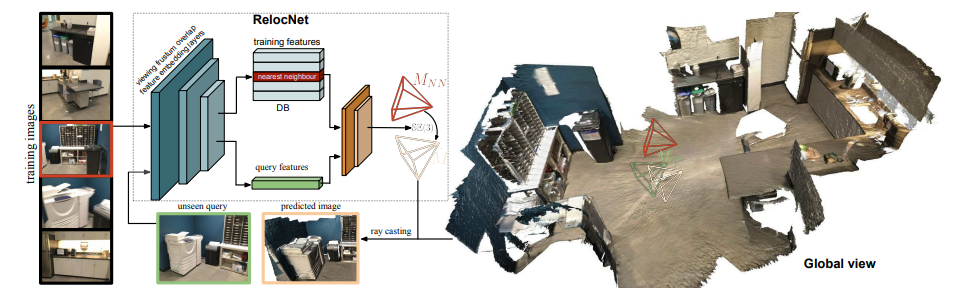
\includegraphics[width=\textwidth]{pics/Chapter2/relocnet.png}
    \caption{Minh họa kiến trúc mô hình RelocNet \cite{10.1007/978-3-030-01264-9_46}}
\end{figure}
Để giải quyết vấn đề hiệu suất giới hạn của các phương pháp hồi quy vị trí tương đối tiền nhiệm do sử dụng cùng đặc trưng cho cả hai bước truy xuất và hồi quy, CamNet \cite{9008579} đề xuất một quy trình chia làm ba bước: truy xuất thô, truy xuất mịn và hồi quy vị trí. Kiến trúc mô hình được xây dựng dựa trên kiến trúc Siamese với ba nhánh mỗi bước. Kiến trúc thô-sang-mịn này đã mang lại những cải tiến về hiệu suất hồi quy cũng như khả năng mở rộng. Hàm mất mát của CamNet lấy ý tưởng dựa trên RelocNet, được định nghĩa như sau:
\begin{center}
$l = l_{frustum} + l_{angle} + l_{triplet} + l_{PFR} + l_{PRP}$
\end{center}
\begin{figure}[H]
    \centering
    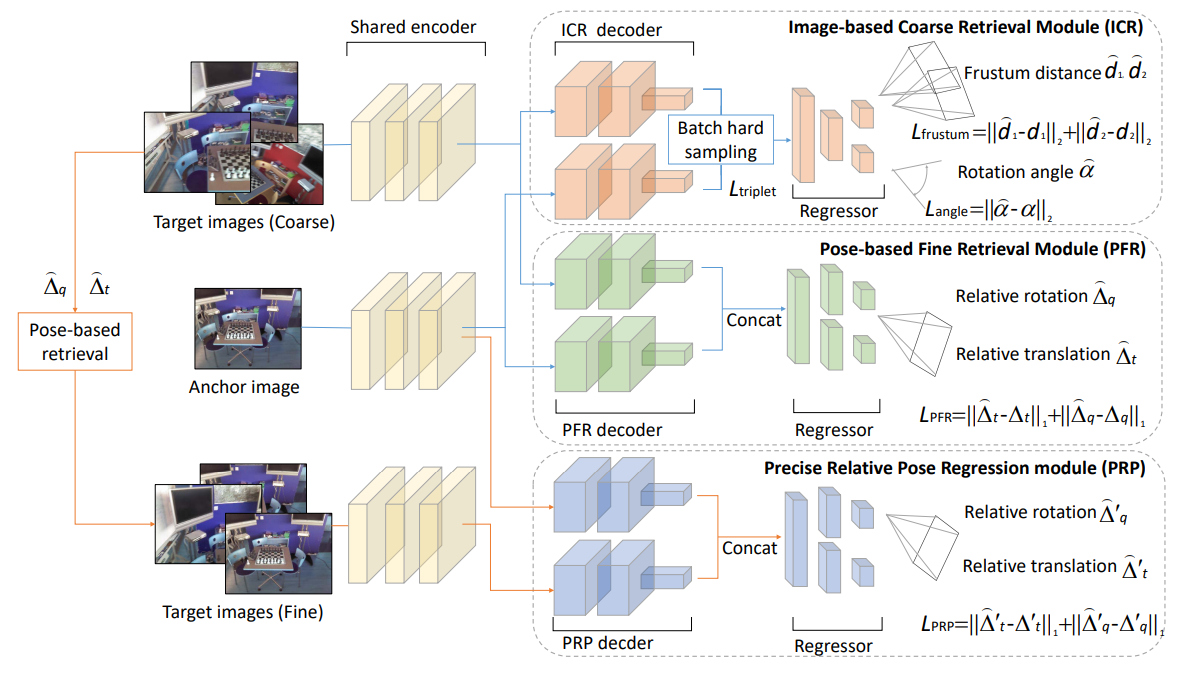
\includegraphics[width=0.7\textwidth]{pics/Chapter2/camnet.png}
    \caption{Minh họa kiến trúc mô hình CamNet \cite{9008579}}
\end{figure}
Qunjie Zhou và những cộng sự \cite{zhou2020learn} sau khi phân tích các phương pháp hồi quy vị trí dựa trên việc truy xuất ảnh đã đề xuất một kiến trúc mới sử dụng ma trận thiết yếu và RANSAC để tính toán vị trí tuyệt đối. Một mạng Siamese ResNet34 với một lớp tìm sự tương ứng cố định (EssNet) và một lớp tìm sự tương ứng đồng thuận lân cận (NC-EssNet) được học để tạo ra một bản đồ điểm tương ứng phục vụ cho mục đích hồi quy về sau của ma trận thiết yếu. Hàm mất mát cải tiến khoảng cách Euclidean giữa ma trận thiết yếu với hai véc-tơ 9 chiều.
\begin{center}
$l_{ess}(E^*, E) = \left \| e - e^* \right \|_2$
\end{center}
\begin{figure}[H]
    \centering
    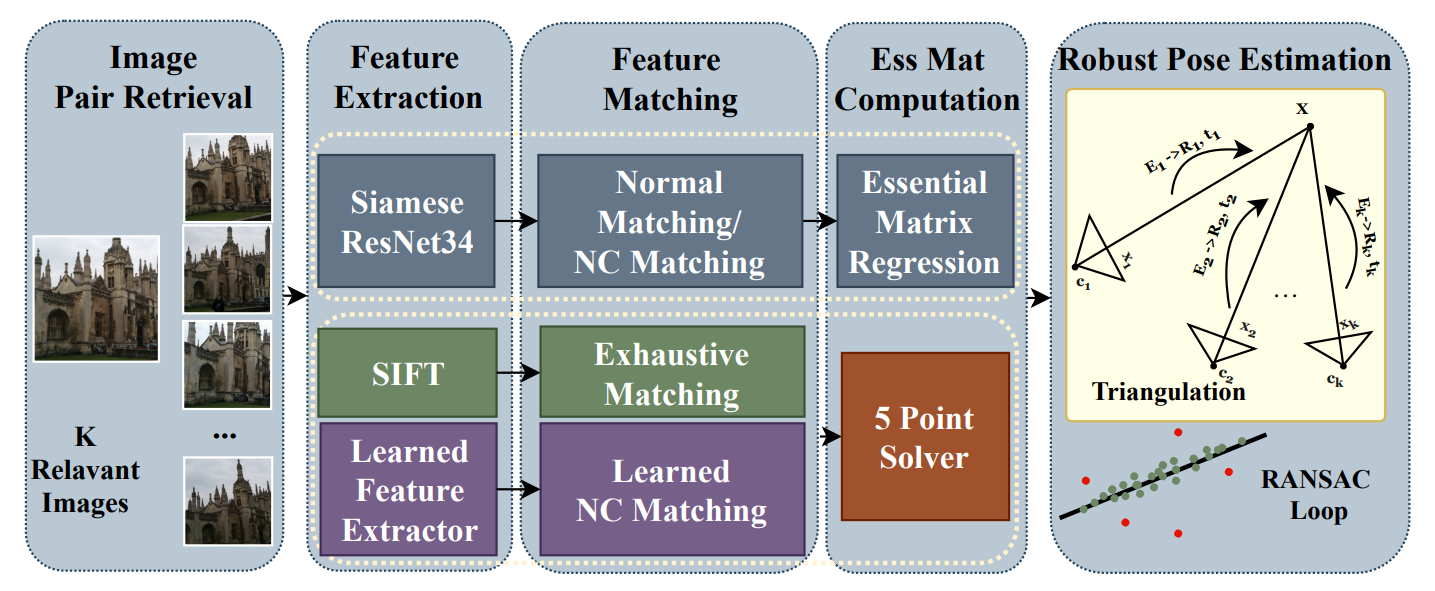
\includegraphics[width=0.7\textwidth]{pics/Chapter2/essnet.png}
    \caption{Minh họa kiến trúc mô hình EssNet \cite{zhou2020learn}}
\end{figure}

\subsubsection*{Hồi quy vị trí tương đối thông qua mạng CNN ngầm - Relative camera pose regression through implicit CNN}
Để tránh việc phải thu thập và xây dựng một kho dữ liệu khổng lồ cũng như tốn kém thời gian thử nghiệm, một số phương pháp tìm cách hồi quy vị trí tương đối của máy ảnh thông qua một mạng Nơ-ron tích chập ngầm.

Relative NN \cite{melekhov2017relative} đề xuất một phương pháp đầu-cuối để hồi quy vị trí tương đối giữa hai máy ảnh bằng hai ảnh đầu vào. Kiến trúc mô hình là một mạng Nơ-ron hỗn hợp Siamese hai nhánh sử dụng mạng AlexNet đã được huấn luyện từ trước được dùng cho việc hồi quy với hàm mất mát Euclidean cố định.
\begin{figure}[H]
    \centering
    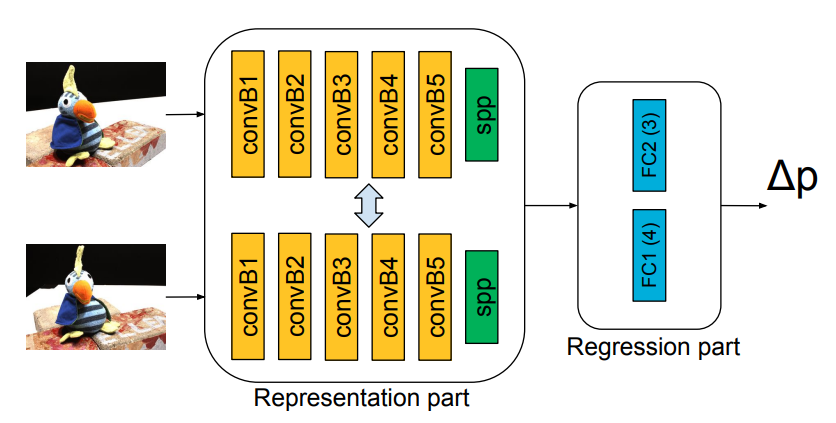
\includegraphics[width=0.7\textwidth]{pics/Chapter2/relativenn.png}
    \caption{Minh họa kiến trúc mô hình Relative Neural Network \cite{melekhov2017relative}}
\end{figure}
AnchorNet \cite{saha2018improved} tìm cách khắc phục vấn đề định vị bằng cách định nghĩa các địa danh thành các điểm mốc để học các điểm mốc tương đối của ảnh đầu vào cũng như độ lệch của chúng. Mô hình đa nhiệm bao gồm việc phân loại hình ảnh truy vấn đầu vào theo các điểm mốc cụ thể và tìm sự chênh lệch so với điểm mốc đã phân loại, điều này dẫn đến việc hình thành hàm mất mát. $\hat{C}$, $X$, và $Y$ đại diện cho kết quả phân loại và sự chênh lệch với sự thật nền tảng.
\begin{center}
$l = \sum_i[(X_i - \hat{X}_i)^2 + (Y_i - \hat{Y}_i)^2]\hat{C}^i$
\end{center}
\begin{figure}[H]
    \centering
    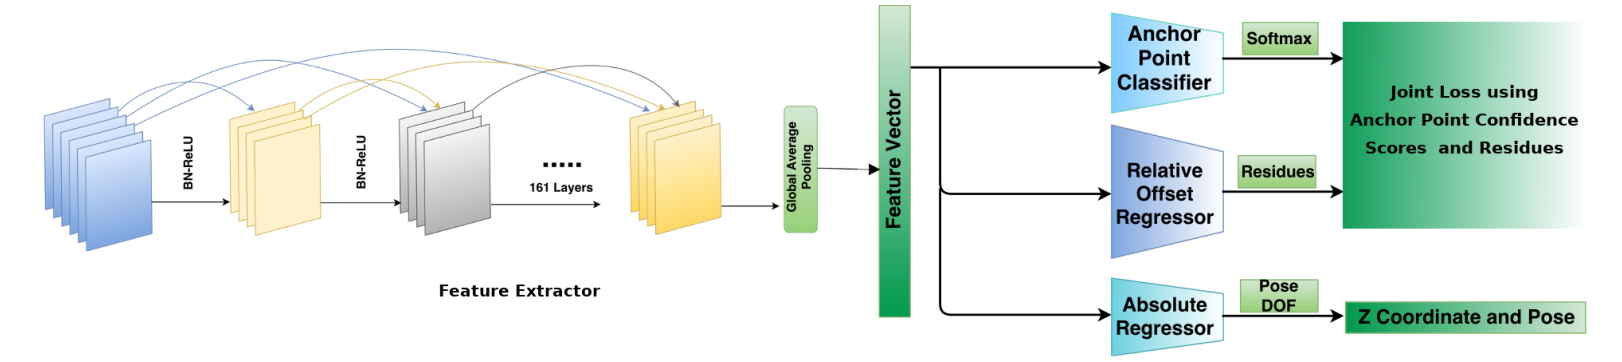
\includegraphics[width=0.7\textwidth]{pics/Chapter2/anchornet.png}
    \caption{Minh họa kiến trúc mô hình AnchorNet \cite{saha2018improved}}
\end{figure}

\subsubsection*{}
Nhận thấy các phương pháp tái bản địa hóa trực quan (Visual Relocalization) hiện tại đều cần một kho dữ liệu ảnh khổng lồ nhằm mục đích xây dựng một mô hình 3 chiều cho một khung cảnh nhất định, một nhóm nghiên cứu \cite{arnold2022mapfree} đề xuất phương pháp mang tên "Tái định vị không cần bản đồ (Map-free Relocalization)" với việc chỉ sử dụng duy nhất một ảnh làm đầu vào mà không cần phải xây dựng mô hình 3 chiều cho cảnh. \cite{arnold2022mapfree} đã đề xuất hai phương pháp khác nhau để có thể xác định vị trí, góc quay chính xác từ một ảnh: thứ nhất là tận dụng ma trận thiết yếu kết hợp với các kỹ thuật tìm sự tương ứng giữa đặc trưng ảnh, thứ hai là hồi quy vị trí tương đối.
\begin{figure}[H]
    \centering
    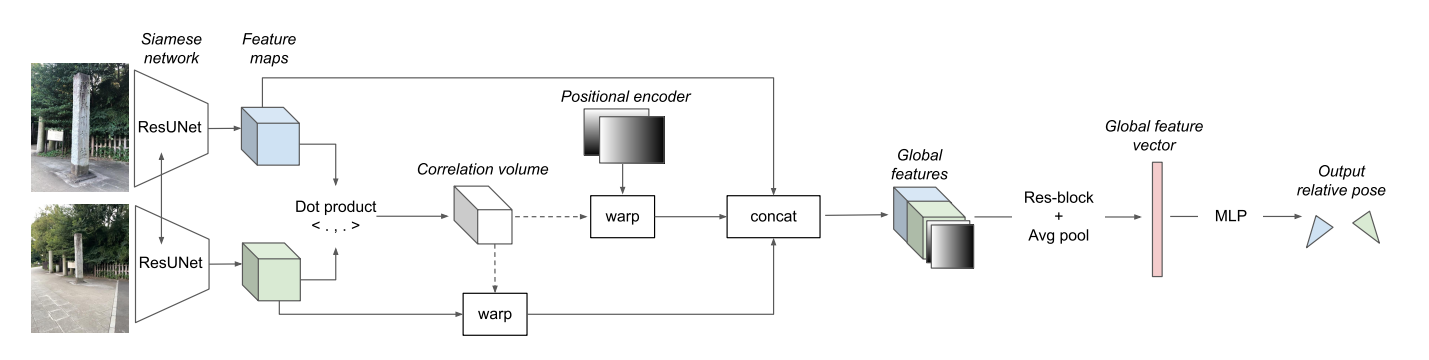
\includegraphics[width=0.7\textwidth]{pics/Chapter2/mapfreeRPR}
    \caption{Minh họa kiến trúc mô hình hồi quy vị trí tương đối của Map-free \cite{arnold2022mapfree}}
\end{figure}

\subsubsection*{Kết luận}
Để thực hiện tác vụ hồi quy vị trí tương đối, các phương pháp dựa trên truy xuất ảnh \cite{laskar2017camera, 10.1007/978-3-030-01264-9_46, 9008579, zhou2020learn} tận dụng một quy trình nhiều bước để lấy được vị trí tuyệt đối với bước truy xuất ảnh làm trọng tâm. NNnet \cite{laskar2017camera} là công trình đầu tiên đề xuất một phương pháp hồi quy vị trí tương đối dựa trên truy xuất ảnh, với RelocNet \cite{10.1007/978-3-030-01264-9_46} tìm cách cải tiến NNet với việc học liên tục thước đo với mục đích học các đặc trưng ảnh toàn cục kết hợp góc nhìn chóp cụt của máy ảnh để cải thiện kết quả. CamNet \cite{9008579} đề xuất một quy trình chia làm ba bước: truy xuất thô, truy xuất mịn và hồi quy vị trí với ba nhánh CNN mỗi bước và đã mang lại những cải tiến về hiệu suất hồi quy cũng như khả năng mở rộng. 

Trong khi đó các phương pháp dựa trên CNN \cite{melekhov2017relative, saha2018improved, arnold2022mapfree} lại đề xuất một hướng giải quyết để hồi quy trực tiếp vị trí tương đối ngay trong mạng nơ-ron. Relative NN \cite{melekhov2017relative} đề xuất một mô hình đầu-cuối Siamese hai nhánh để hồi quy vị trí tương đối giữa hai ảnh đầu vào. AnchorNet \cite{saha2018improved} tìm cách khắc phục vấn đề định vị bằng cách định nghĩa các địa danh thành các điểm mốc để học các điểm mốc tương đối của ảnh đầu vào cũng như độ lệch của chúng. Map-free \cite{arnold2022mapfree} đề xuất việc không sử dụng ảnh để tái kiến trúc lại cảnh, đồng thời cung cấp hai phương hướng để hồi quy vị trí từ một ảnh.


\subsection{Tái tạo kiến trúc từ chuyển động - Structure From Motion}

\section{Phân tích và tổng hợp}
Về các phương pháp hồi quy vị trí máy ảnh, các nghiên cứu cho thấy hiệu suất dự đoán vị trí vẫn chưa thể vượt qua các phương pháp tái kiến trúc từ chuyển động. Các phương pháp hồi quy vị trí máy ảnh vẫn còn đang trên đà phát triển tuy nhiên vẫn gặp nhiều khó khăn với việc giải quyết các đặc trưng cục bộ trùng lặp cũng như việc tiêu tốn nhiều tài nguyên tính toán. Hầu hết công trình tập trung vào các điểm đặc trưng có độ chắc chắn cao hoặc mô tả đặc trưng chính xác dưới điều kiện mang tính thử thách cao. Ngoài ra, phần lớn các phương pháp được đề xuất chỉ có thể áp dụng trong một phạm vi nhỏ và vẫn chưa chứng tỏ được hiệu suất trên những tập dữ liệu có quy mô lớn.
	
\section{Một số tập dữ liệu phổ biến được sử dụng}
\subsection{Tập dữ liệu trong không gian nhỏ}
\subsubsection*{7Scenes}
Tập dữ liệu 7-Scenes \cite{6619221} bao gồm các ảnh RGB-D thuộc bảy khung cảnh khác nhau được chụp từ một máy ảnh cầm tay Kinect RGB-D ở độ phân giải 640x480. Bảy khung cảnh bap gồm: "Chess", "Fire", "Heads", "Office", "Pumpkin", "RedKitchen" và "Stairs". Với mỗi cảnh sẽ có vài chuỗi khung ảnh RGB-D. Mỗi chuỗi bao gồm khoảng từ 1000 đến 5000 khung ảnh. Mỗi khung sẽ gồm: ảnh màu, độ sâu và vị trí.
\begin{figure}[H]
    \centering
    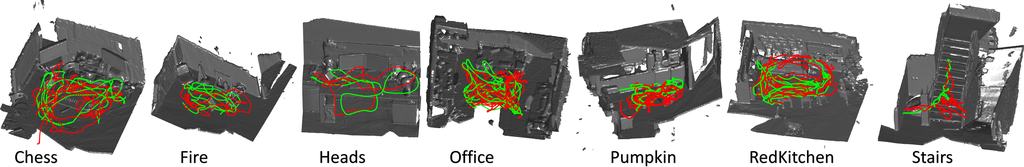
\includegraphics[width=\textwidth]{pics/Chapter2/7scenes.png}
    \caption{Minh họa tập dữ liệu 7-Scenes \cite{6619221}}
\end{figure}
\subsubsection*{Cambridge Landmark}
Tập dữ liệu Cambridge Landmarks \cite{kendall2016posenet} là một tập dữ liệu định vị thành thị bao gồm năm khung cảnh khác nhau. Các yếu tố dày đặc quan trọng như phương tiện giao thông hay người đi bộ cũng xuất hiện trong tập dữ liệu này, ngoài ra dữ liệu cũng được thu thập ở nhiều thời điểm trong ngày đại diện cho các yếu tố ánh sáng và điều kiện thời tiết khác nhau. Cambridge Landmarks được tạo ra nhờ vào việc áp dụng các kỹ thuật tái tạo kiến trúc từ chuyển động. Một chiếc điện thoại thông minh Google LG Nexus 5 được một người đi bộ trên phố sử dụng để ghi lại đoạn phim chất lượng cao cho mỗi cảnh. Mỗi đoạn phim sau đó sẽ được lấy mẫu với tần số 2Hz để trích xuất ảnh cho quy trình tái tạo kiến trúc từ chuyển động. Mỗi vị trí máy ảnh sẽ cách nhau khoảng 1m.
\begin{figure}[H]
    \centering
    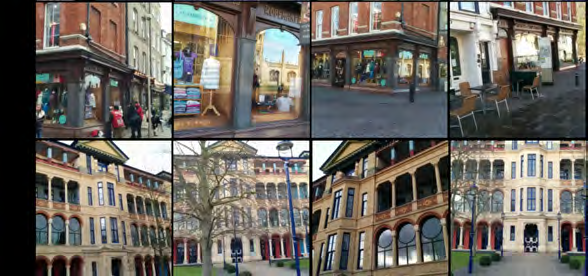
\includegraphics[width=\textwidth]{pics/Chapter2/cambridge.png}
    \caption{Minh họa tập dữ liệu Cambridge Landmarks \cite{kendall2016posenet}}
\end{figure}
\subsubsection*{Niantic Map-free Relocalization Dataset}
Tập dữ liệu Niantic Map-free Relocalization \cite{arnold2022mapfree} là một tập dữ liệu được thu thập chủ yếu để giúp ích cho phương pháp định vị Map-free \cite{arnold2022mapfree}. Tập dữ liệu bao gồm 655 cảnh bên ngoài với mỗi cảnh sẽ chứa một "địa điểm đáng chú ý" như một pho tượng, cổng, bảng hiệu,... sao cho địa điểm đó phải được xác định rõ trong một bức ảnh. Các cảnh được chia ra thành 460 cảnh phục vụ cho tác vụ huấn luyện, 65 cảnh phục vụ cho tác vụ kiểm tra quy trình huấn luyện và 130 cảnh phục vụ cho quá trình kiểm thử. Mỗi ảnh trong tập huấn luyện đều được gắn kèm vị trí tuyệt đối. Với tập kiểm thử và kiểm tra quy trình, mỗi cảnh sẽ được kèm theo một ảnh đại diện cũng như vị trí tuyệt đối tại cảnh. Ngoài ra, ma trận tham số nội tại của máy ảnh cũng được gắn kèm theo mỗi ảnh trong tập dữ liệu.
\begin{figure}[H]
    \centering
    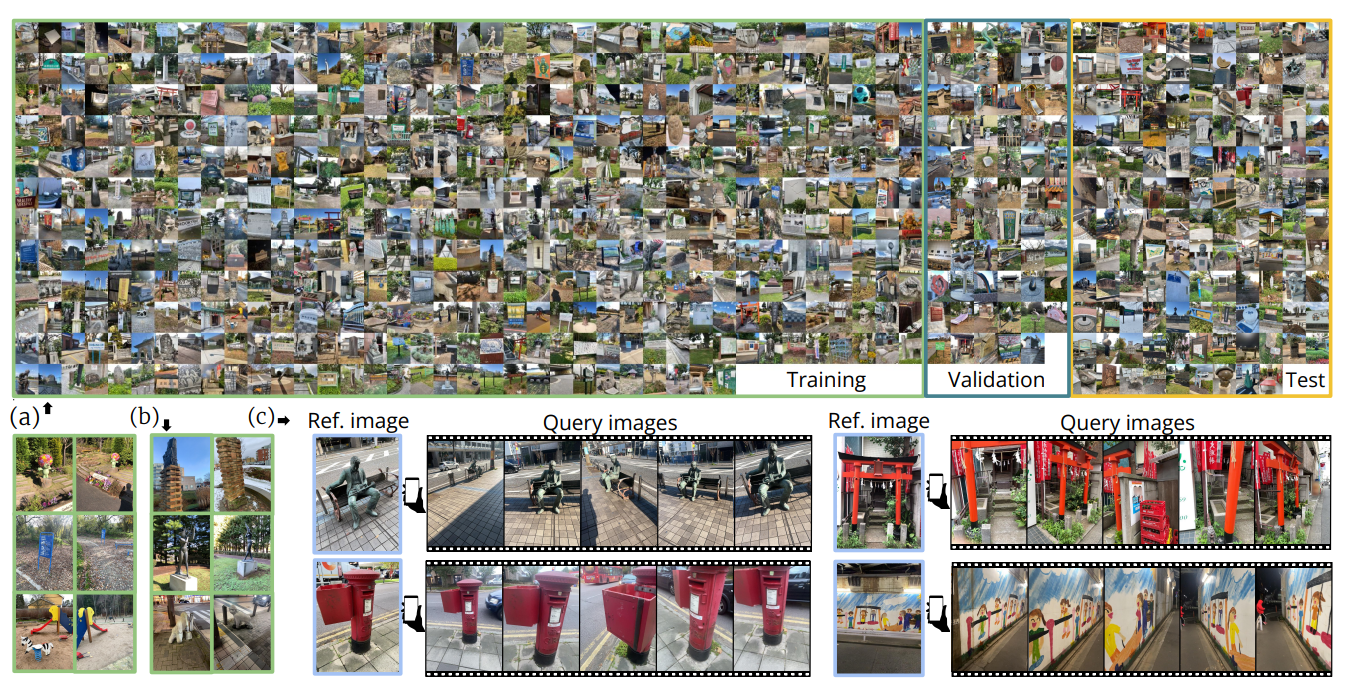
\includegraphics[width=\textwidth]{pics/Chapter2/niantic.png}
    \caption{Minh họa tập dữ liệu Niantic Map-free Relocalization \cite{arnold2022mapfree}}
\end{figure}
\subsection{Tập dữ liệu thành thị}
\subsubsection*{Aachen Day-Night}
Tập dữ liệu Aachen Day-Night \cite{Sattler2012ImageRF} bao gồm 14.607 ảnh được chụp với nhiều máy ảnh khác nhau bao phủ cả thành phố Aachen thuộc quốc gia Đức. Các ảnh dữ liệu được chụp ở nhiểu thời điểm trong ngày và trong năm, cụ thể là khoảng thời gian trong 2 năm. Hệ quả mang lại là tập dữ liệu bao phủ nhiều điều kiện ngoại cảnh như thời tiết, ánh sáng cũng như sự thay đổi của công trình kiến trúc trong khu vực.
\begin{figure}[H]
    \centering
    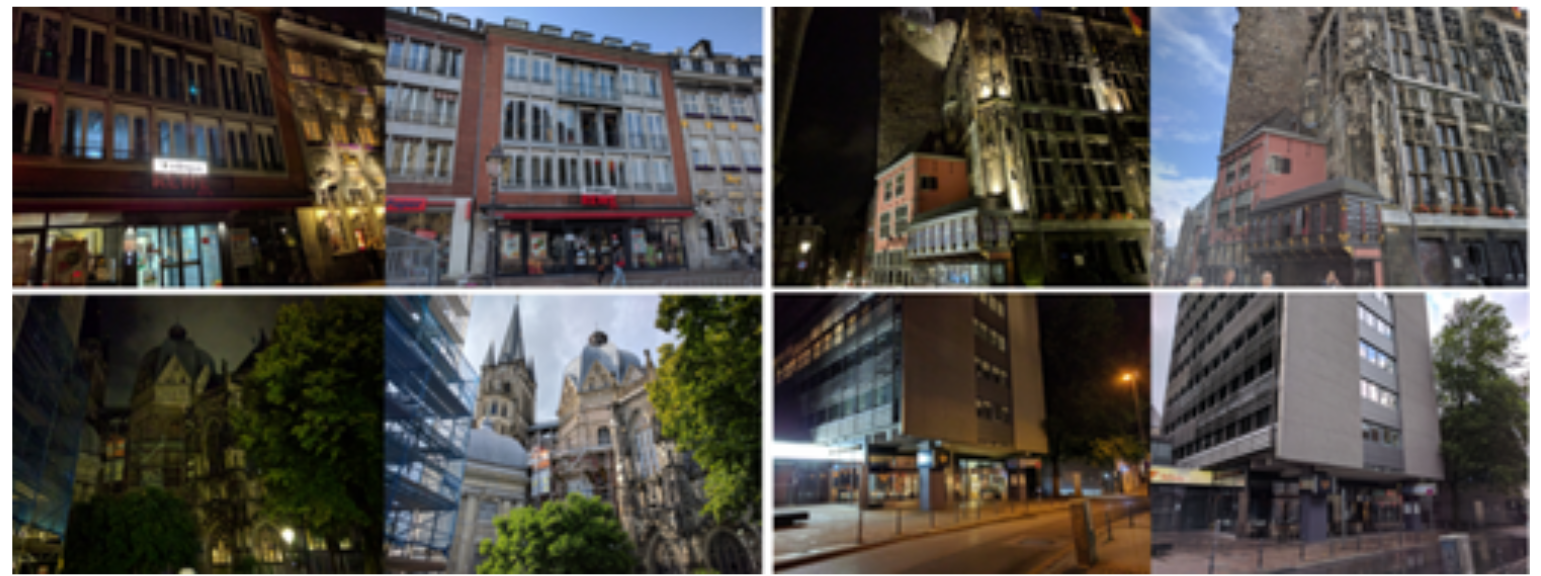
\includegraphics[width=\textwidth]{pics/Chapter2/aachen.png}
    \caption{Minh họa tập dữ liệu Aachen Day-Night \cite{Sattler2012ImageRF}}
\end{figure}
\subsubsection*{Pittsburgh 250k}
Tập dữ liệu Pittsburgh 250k \cite{6618963} là một tập dữ liệu tương đối rộng bao phủ thành phố Pittsburgh của Mỹ. Đây là một tập dữ liệu tương đối phổ biến trong thị giác máy tính, cụ thể là ở tác vụ nhận điện địa điểm trực quan, truy xuất ảnh và bản địa hóa trực quan.

\subsubsection*{GSV-Cities}
Tập dữ liệu GSV-Cities \cite{Ali_bey_2022} bao phủ một vùng địa lý cực kỳ rộng lớn với hơn 40 thành phố xuyên lục địa trong khoảng thời gian 14 năm liên tục. GSV-Cities chứa khoảng hơn 530.000 ảnh - khoảng hơn 62.000 vị trí. Mỗi vị trí sẽ có khoảng từ 4 đến 20 ảnh. Đồng thời mỗi vị trí sẽ cách nhau một khoảng ít nhất 100m.
\begin{figure}[H]
    \centering
    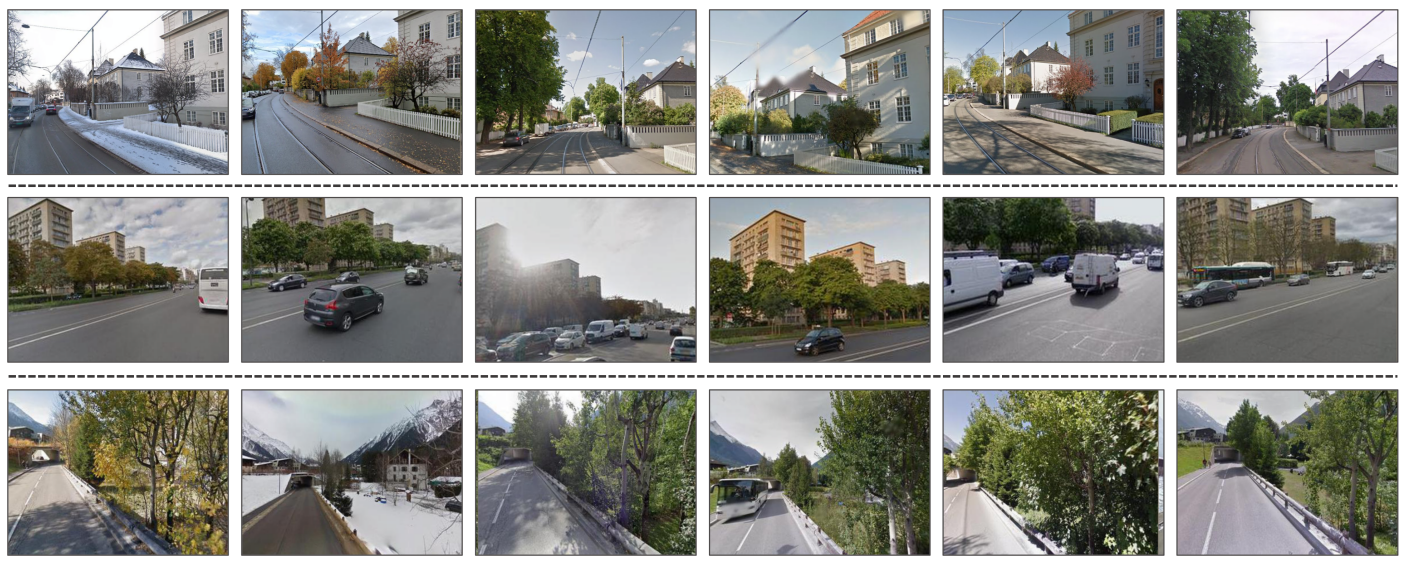
\includegraphics[width=\textwidth]{pics/Chapter2/gsv.png}
    \caption{Minh họa tập dữ liệu GSV-Cities \cite{Ali_bey_2022}}
\end{figure}

\subsubsection*{SF-XL}
Tập dữ liệu San Francisco Extra Large (SF-XL) \cite{berton2022rethinking} được tạo nên từ 3.43 triệu ảnh 360 độ thu thập từ kho ảnh Google Streetview. Các ảnh này sau đó được cắt ra thành 41.2 triệu ảnh. Mỗi ảnh cắt ra đều được gắn nhãn 6DoF (bao gồm cả GPS). Dữ liệu được thu thập từ năm 2009 đến năm 2021, dẫn đến việc tập dữ liệu bao phủ nhiều điều kiện ngoại cảnh như thời tiết, ánh sáng cũng như sự thay đổi của công trình kiến trúc trong khu vực.
\begin{figure}[H]
    \centering
    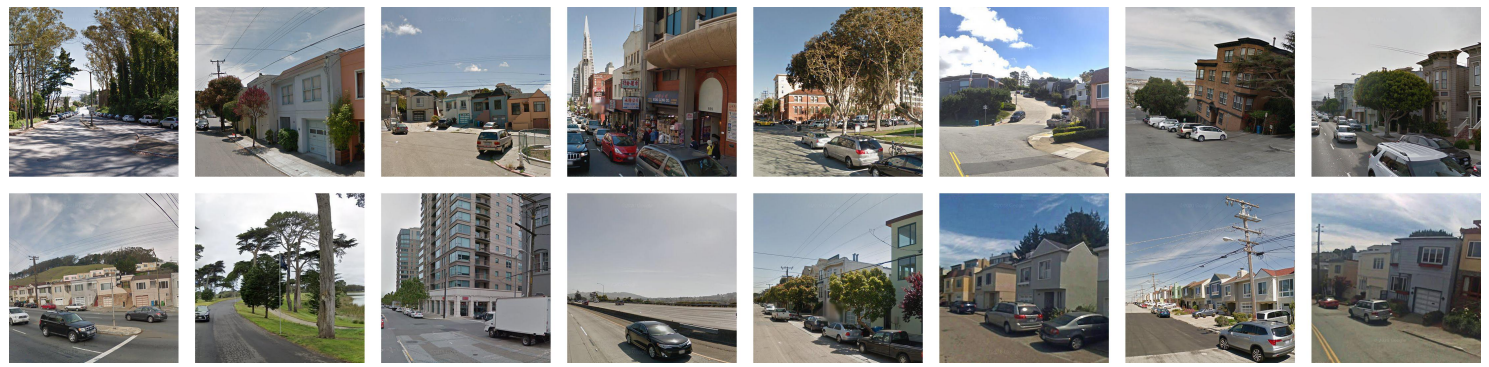
\includegraphics[width=\textwidth]{pics/Chapter2/sfxl.png}
    \caption{Minh họa tập dữ liệu San Francisco Extra Large \cite{berton2022rethinking}}
\end{figure}


\chapter{PHƯƠNG PHÁP ĐỀ XUẤT}

\section{Tổng quan}
\subsection{Kiến trúc pipeline}
Sau khi đã xác định những mô hình baseline sẽ sử dụng trong hệ thống, chúng tôi tiến hành thiết kế một kiến trúc phù hợp để có thể kết hợp hai hướng tiếp cận trong một pipeline hoàn chỉnh. Pipeline sẽ có kiến trúc như được mô tả trong hình 3.1 với hai module lớn là module \textbf{nhận diện địa điểm trực quan - Visual Place Recognition(VPR)} với baseline là mô hình MixVPR và module \textbf{hồi quy tư thế tương đối - Relative Pose Regression(RPR)} với baseline là mô hình Mapfree 2D-2D. Module VPR sẽ giúp chọn ra ảnh tham khảo từ tập dữ liệu mô tả khu vực đang hoạt động làm cột mốc để cho module RPR có thể hồi quy ra được vị trí của ảnh truy vấn so với ảnh tham khảo.

\begin{figure}[htbp]
  \centering
  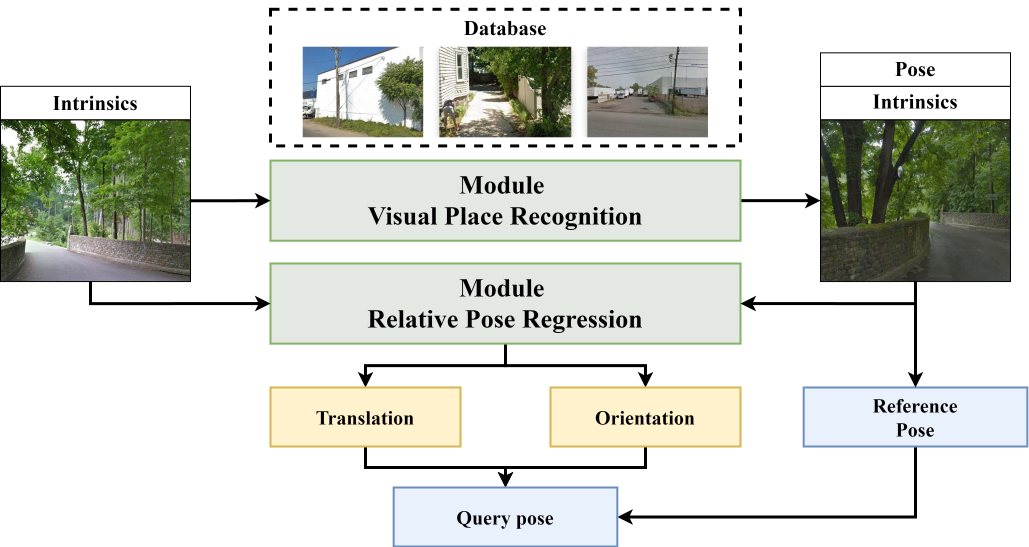
\includegraphics[width=\textwidth]{pics/Proposal/arch.png}
  % \includesvg[scale=0.3]{pics/Proposal/arch.svg}
  \caption{Kiến trúc tổng quan của pipeline định vị trực quan được đề xuất}
\end{figure}

Gọi $I$ là ảnh mà người dùng chụp từ camera và sẽ được dùng làm ảnh truy vấn cho pipeline đề xuất của chúng tôi. Trước hết, pipeline sẽ nhận $I$ làm đầu vào cho MixVPR. Từ ảnh đầu vào $I$, sau khi qua các giai đoạn xử lý, MixVPR sẽ trả về một đoạn mã hóa biểu diễn cho nội dung của ảnh. Với đoạn mã hóa này, pipeline tiến hành so sánh với giá trị mã hóa của các ảnh trong cơ sở dữ liệu và tìm ra ảnh có sự tương đồng cao nhất với ảnh nhận vào $I$ gọi là $I_0$.

Bước tiếp theo, pipeline tiếp tục truyền cả ảnh nhận vào $I$ và ảnh được truy xuất $I_0$ cho mô hình tương quan 2D - 2D của Map-free Relocalization \cite{arnold2022mapfree}. Với đầu vào là cặp ảnh $(I, I_0)$, những cặp đặc trưng tương quan giữa hai ảnh sẽ được xác định tương ứng với mỗi hình. Sau đó, Essential Matrix $E$ giữa 2 ảnh sẽ được ước tính. Essential Matrix sau đó sẽ được phân giải thành ma trận thể hiện góc quay chênh lệch $R$ và một vector đơn vị độ dịch vị trí $\hat{t}$. Từ các cặp đặc trưng và độ sâu của ảnh, mô hình tiến hành một bước chiếu 3D để tính toán giá trị tỷ lệ $s$ của vector độ dịch vị trí. Cuối cùng, tư thế thực của camera sẽ được xác định bằng tư thế thực của ảnh tham khảo và độ lệch giữa ảnh tham khảo và ảnh truy vấn $(R,s*\hat{t})$.

\subsection{Dữ liệu đầu vào và đầu ra}
Mô hình sẽ nhận vào ảnh $I$, có định dạng là một ảnh RGB. Sau đó, ảnh $I$ sẽ được tiền xử lý, gồm các bước đưa về kích thước 320x320 và chuẩn hóa các điểm ảnh trên hình, trước khi được đưa vào mô hình chính. Lưu ý, mô hình kết hợp sẽ cần ảnh phải mang thông tin tham số nội tại của máy ảnh nhằm thực hiện bước hồi quy tư thế.

Qua quá trình mô phỏng lại bài toán nhận diện địa điểm trực quan, mô hình sẽ thu được $k$ cặp ảnh có độ tương đồng cao, gồm ảnh truy vấn ban đầu và ảnh tham khảo truy xuất được. Từng cặp ảnh trong $k$ cặp này sẽ được đưa vào bộ phận hồi quy tư thế tương đối tiếp theo. Có được tư thế của ảnh $I$ so với $k$ ảnh tham khảo có độ tương đồng cao nhất, mô hình sẽ chọn ra kết quả cuối cùng dựa vào độ đáng tin cậy $C$ được xác định ở \textbf{bộ phận xác định Essential Matrix}.

Định dạng đầu ra của mô hình sẽ gồm hai tập vector $R$ và $t$, lần lượt thể hiện góc quay và vị trí chụp ảnh trong không gian 3D. Cụ thể, hai vector sẽ có dạng:
\begin{itemize}
  \item \textbf{Vector góc quay $R$} sẽ có định dạng của một Quaternion, gồm 4 số là $(q_w, q_x, q_y, q_z)$. Quaternion có thể được dùng để biểu diễn góc quay trong không gian 3D và có thể dùng để thay thế ma trận xoay 3x3, nhằm có thể thể hiện và kết hợp các phép quay một cách dễ dàng hơn. Công thức biểu diễn một góc quay là
        \begin{equation}
          q=q_w + i*q_x + j*q_y + k*q_z,
        \end{equation}
        với $q_w, q_x, q_y, q_z$ là các số thực với $i,j,k$ là những vector đơn vị trực giao lẫn nhau. Quaternion có thể được biến đổi theo dạng trục quay và góc quay, có thể được biểu diễn bởi hai thành phần là vector đơn vị biểu diễn trục của góc quay, $(\hat{x},\hat{y},\hat{z})$ và độ quay quanh trục, $\theta$.
        \begin{figure}[H]
          \centering
          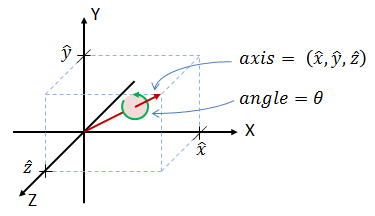
\includegraphics[scale=1]{pics/Proposal/axis-angle.png}
          \caption{Minh họa cách biểu diễn trục quay và góc quay \cite{quaternion}}
        \end{figure}
        Quaternion có thể được ước tính từ cách biểu diễn trục quay và góc quay theo công thức
        \begin{equation}
          \begin{aligned}
             & q_w=\cos \left(\frac{\theta}{2}\right)         \\
             & q_x=\hat{x} \sin \left(\frac{\theta}{2}\right) \\
             & q_y=\hat{y} \sin \left(\frac{\theta}{2}\right) \\
             & q_z=\hat{z} \sin \left(\frac{\theta}{2}\right),
          \end{aligned}
        \end{equation}
        với tập các giá trị $q_w, q_x, q_y, q_z$ có độ lớn là 1, dẫn đến tập các giá trị này sẽ có 3 độ tự do, 3DoF.
  \item \textbf{Vector vị trí $t$} sẽ có 3 giá trị là $t_x,t_y,t_z$ lần lượt thể hiện các giá trị kinh độ, vĩ độ và độ cao của vị trí chụp ảnh trong không gian thực tế. Vector thể hiện vị trí có cách biểu diễn đơn giản và dễ hiểu hơn so với góc quay. Ngoài ra, do biểu diễn không gian 3D thực tế nên vector thể hiện vị trí sẽ có 3 độ tự do.
\end{itemize}

\section{Module nhận diện địa điểm trực quan - VPR}
Module VPR của pipeline được phát triển dựa trên mô hình MixVPR được giới thiệu trong bài \cite{alibey2023mixvpr}. Đây là một phương pháp tổng hợp đặc trưng. Từ kết quả đặc trưng xác định được từ mô hình backbone, MixVPR giới thiệu một phương pháp tổng hợp mới, được thực hiện bởi khối Feature Mixer, một cấu trúc đặc biệt được xây dựng dựa trên mô hình MLP-Mixer \cite{tolstikhin2021mlpmixer}. Mô hình MixVPR sử dụng những khối này nhằm tích hợp thông tin toàn cục vào các đặc trưng. Nhờ vào kiến trúc nhẹ của khối Feature Mixer, hướng tiếp cận này cho phép MixVPR đạt hiệu năng cao ở tập dữ liệu thành thị phạm vi rộng mà không có tác động tài nguyên lớn.

\subsection{Kiến trúc}

\begin{figure}[H]
    \centering
    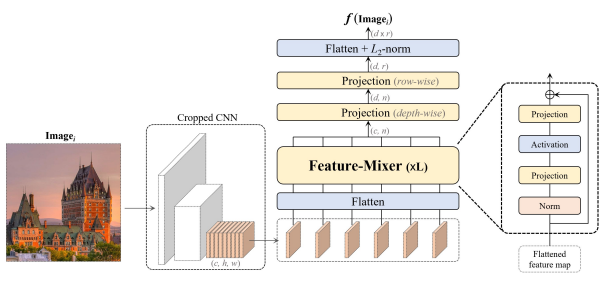
\includegraphics[width=\textwidth]{pics/Proposal/mixvpr.png}
    \caption{Tổng quan quá trình hoạt động của MixVPR \cite{alibey2023mixvpr}}
\end{figure}

\subsubsection{Mô hình backbone trích xuất đặc trưng thô}
Khi ảnh truy vấn $I$ được đưa vào, mô hình CNN backbone được sử dụng để trích xuất ra những chi tiết mang thông tin cần thiết. Mô hình cơ sở được huấn luyện trên những tập dữ liệu hình ảnh đa dạng, nhằm có thể phát hiện ra những đặc trưng quan trọng phục vụ các tác vụ liên quan đến thị giác máy tính. Trong kiến trúc đề xuất, mô hình cơ sở được cắt ở giữa, nhằm thu được tập những bản đồ đặc trưng $F$ có định dạng $F \in R^{c \cdot h \cdot w}$.

Ở những phương pháp trước đây như NetVLAD \cite{arandjelovic2016netvlad} và PatchNetVLAD \cite{hausler2021patchnetvlad}, những lớp bản đồ đặc trưng thuộc $F$ được xem như là một mô tả tương ứng với một miền tiếp nhận cho một khu vực trong ảnh ban đầu. Ngược lại, MixVPR xem $F$ như một tập các bản đồ đặc trưng 2D có kích thước $h \cdot w$, miêu tả toàn ảnh. Đây là một cách biểu diễn ảnh nhỏ, nhẹ và thống nhất hơn trong điều kiện thay đổi về ánh sáng và góc nhìn, thay cho việc lưu trữ từng điểm ảnh.
\begin{equation}
    F = \{X^{i}\},
\end{equation}
với $i \in \left[1,..,c\right]$ và $X^{i}$ tương ứng với bản đồ kích hoạt thứ $i$ ở F.

Mỗi bản đồ đặc trưng $X^{i}$ thuộc tập $F$ sau đó được được định dạng lại thành ma trận một chiều có dạng $X_{flat}^{i} \in R^{h*w}$, thu được được $F_{flat} \in R^{c \cdot n}$ với $n = h*w$.

\subsubsection{Khối tổng hợp Feature Mixer}
Tiếp theo, tập hợp của những bản đồ đặc trưng $F_{flat}$ lần lượt được đưa qua $L$ khối Feature Mixer, được phát triển trên cấu trúc mạng MLP. Mỗi khối Feature Mixer nhận vào từng bản đồ đặc trưng $X_{flat}^{i}$ một chiều và tích hợp thông tin về mối liên kết giữa các giá trị của $X_{flat}^{i}$ lên chính nó thông qua cách sau:
\begin{equation}
    \begin{aligned}
        X^{i} & \leftarrow Norm(X^{i})             \\
        X^{i} & \leftarrow W_2(\sigma(W_1 X^{i})),
    \end{aligned}
\end{equation}
với $W_1$ và $W_2$ là trọng số của hai lớp liên kết đầy đủ, cấu tạo nên MLP và $\sigma$ là hàm tạo sự phi tuyến tính cho quá trình xử lý (ReLU). Kỹ thuật nối tắt được sử dụng để nối đầu vào đã qua lớp chuẩn hóa với đầu ra nhằm giúp độ dốc trong quá trình huấn luyện có thể được truyền tải dễ hơn, cải thiện quá trình huấn luyện. Kết quả đầu ra của khối Feature Mixer được giữ định dạng giống như dữ liệu đầu vào, có dạng $R^{h*w}$.

Mục đích của việc sử dụng Feature Mixer là để tận dụng khả năng tổng hợp thông tin từ dữ liệu của các lớp kết nối đầy đủ, thay vì học trên những đặc trưng cục bộ trên ảnh và sử dụng cơ chế tập trung. Ngoài ra, Feature Mixer cũng trả về kết quả có định dạng và kích thước như đầu vào, thay vì giảm dần như những phương pháp tổng hợp dạng phân cấp (kim tự tháp) như trước đây, để mỗi neuron đều có thể biết được thông tin của toàn bộ ảnh. Những lớp MLP trong khối Feature Mixer giúp tích hợp thông tin trên toàn bộ ảnh qua mỗi lần xử lý.

Mỗi khối Feature Mixer sau khi xử lý xong từng bản đồ đặc trưng trong tập $F_{flat} \in R^{c \cdot n}$ ghép kết quả lại, tạo thành $Z \in R^{c \cdot n}$ với cùng kích thước trước khi được đưa vào khối Feature Mixer kế tiếp. Quá trình xử lý tập bản đồ đặc trưng qua các khối Feature Mixer có thể được miêu tả bằng công thức sau:
\begin{equation}
    Z = FM_L(FM_{L-1}(\dots FM_1(F_{flat}))),
\end{equation}
với $FM_i$ là lớp Feature Mixer thứ $i$ trên tổng số $L$ khối và $Z$ là kết quả cuối cùng của quá trình tích hợp thông tin toàn cục.

\subsubsection{Lớp tổng hợp - Aggregation}
Ta có $Z \in R^{c \cdot n}$ với số chiều rất cao do có định dạng được giữ nguyên so với $F_{flat}$. Để giúp giảm bớt số chiều của $Z$ lại sau khi qua khối Feature Mixer, hai lớp kết nối đầy đủ được sử dụng để thực hiện tác vụ tổng hợp lần lượt giữa các giá trị trên cùng một kênh $c$ với nhau và sau đó là giữa các giá trị trong từng bản đồ đặc trưng $X_{flat}^i$. Tác vụ này thực hiện việc tổng hợp có chọn lọc nhằm điều khiển được kích thước của giá trị đầu ra.

Đầu tiên, dữ liệu được tổng hợp số kênh để biến định dạng của $Z$ từ $R^{c \cdot n}$ thành $R^{d \cdot n}$.
\begin{equation}
    Z' = W_d(Transpose(Z)),
\end{equation}
với $W_d$ là trọng số của lớp kết nối đầy đủ đầu tiên và $d$ là định dạng đầu ra sau khi rút gọn số kênh lại, $d<c$.

Sau đó, giá trị trên từng bản đồ đặc trưng được tổng hợp lại, từ định dạng $R^{d \cdot n}$ thành $R^{d \cdot r}$.
\begin{equation}
    O = W_r(Transpose(Z')),
\end{equation}
với $W_r$ là trọng số của lớp kết nối đầy đủ thứ hai và $r$ là định dạng đầu ra của các bản đồ đặc trưng 1D, $r<n$.

Kết quả $O$ cuối cùng, có định dạng là $R^{d \cdot r}$, được ép thành một chiều và chuẩn hóa theo $L_2$ như những phương pháp VPR khác \cite{arandjelovic2016netvlad,berton2022rethinking}. Cuối cùng, từ ảnh đầu vào $I$, mô hình trả về một đoạn mã hóa biểu diễn cho nội dung của ảnh. Đoạn mã hóa này sau đó có thể được dùng để so sánh với giá trị mã hóa của những hình khác nhằm tìm ảnh có độ tương đồng cao nhất với $I$.

\subsubsection{Bộ phận truy vấn ảnh tương đồng}
Sau khi đã có được giá trị mã hóa biễu diễn cho ảnh truy vấn là $O \in R^{d \cdot r}$, mô hình tiến hành tìm kiếm trên tập dữ liệu ảnh miêu tả khu vực đang xét. Cơ chế tìm kiếm được sử dụng là tìm kiếm toàn diện, xét giá trị biểu diễn của từng ảnh. $k$ ảnh có độ tương đồng cao nhất với ảnh truy vấn được chọn để tạo thành các cặp ảnh là đầu ra của bước này.

\begin{figure}[H]
    \centering
    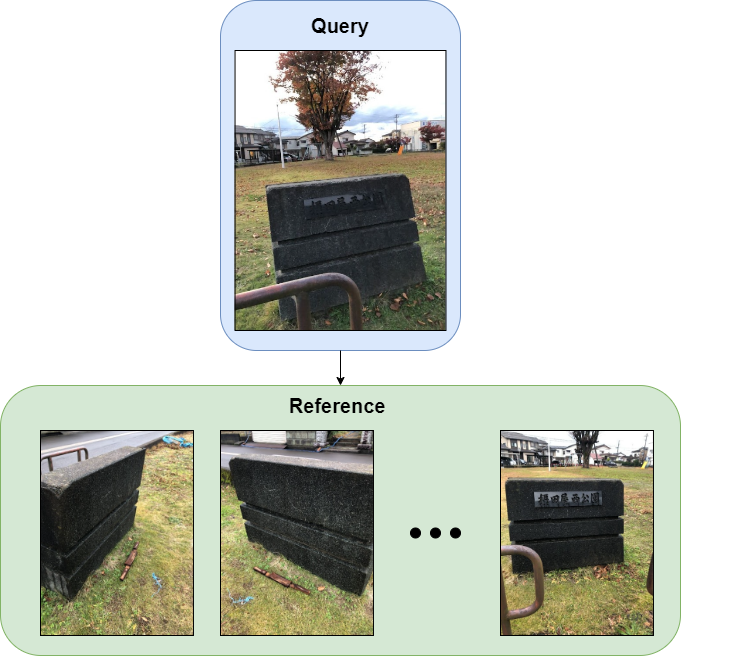
\includegraphics[scale=0.4]{pics/Proposal/query.png}
    \caption[Kết quả của module VPR]{Ảnh truy xuất được từ ảnh truy vấn $I$ ban đầu, từ tập dữ liệu Niantic \cite{arnold2022mapfree}}
\end{figure}


\subsection{Phương pháp hiện thực và triển khai}

\subsubsection{Hiện thực}

Mô hình MixVPR được hiện thực trên framework PyTorch. Mô hình CNN cơ sở của MixVPR được cắt ở lớp áp cuối của mô hình ResNet. Dữ liệu đầu vào cho MixVPR là các ảnh đã được chỉnh về độ phân giải $320x320$ và qua mô hình backbone, một tập các bản đồ đặc trưng có kích thước 20x20 được đưa vào tập $L$ khối Feature Mixer. Thao tác tổng hợp trong khối Feature Mixer sử dụng lớp Linear, theo sau đó là một lớp ReLU để tạo tính phi tuyến tính. Về lớp chuẩn hóa, LayerNorm được sử dụng. Cuối cùng, đầu ra cuối cùng của khối Feature Mixer được tổng hợp xuống một chiều không gian biểu diễn nhỏ hơn sử dụng hai lớp kết nối đầy đủ giữa các kênh với nhau và giữa các giá trị trong mỗi kênh, chứng minh rằng MixVPR là một cấu trúc chỉ sử dụng MLP. Số khối Feature Mixer được sử dụng mặc định là $L=4$.

\subsubsection{Huấn luyện}
Mô hình MixVPR được đánh giá trong bài nghiên cứu sử dụng mô hình ResNet \cite{he2016deep} đã được huấn luyện trên tập ImageNet \cite{krizhevsky2012imagenet} làm cơ sở. Sau đó, mô hình được huấn luyện trên tập dữ liệu GSV-Cities \cite{Ali_bey_2022}. Đối với hàm mất mát, hàm Multi-Similarity Loss \cite{wang2019multi} được sử dụng với lý do đã được chứng minh là hỗ trợ cho ra kết quả tốt nhất với tác vụ VPR \cite{Ali_bey_2022}. Kích thước của một batch có $P = 120$ địa điểm, mỗi địa điểm được miêu tả bởi 4 ảnh, tạo thành một batch có kích thước 480 ảnh. Phương pháp tối ưu giảm độ dốc ngẫu nhiên - SGD được sử dụng với quán tính - momentum là 0.9 với giá trị suy giảm trọng số - weight decay là 0.001. Tốc độ học - learning rate được khởi tạo với giá trị 0.05 và được chia 3 sau mỗi 5 chu kỳ - epoch. Cuối cùng, mô hình được huấn luyện tối đa 30 chu kỳ - epoch với đầu vào là ảnh đã được điều chỉnh kích thước 320x320.

\subsubsection{Phương pháp đánh giá}
Để đánh giá hiệu năng mô hình, 5 tập dữ liệu tiêu chuẩn đã được sử dụng. Pitts250k-test \cite{6618963}, bao gồm 8.000 ảnh truy vấn và 83.000 ảnh tham khảo, được thu thập từ Google Street View và Pitts30k-test \cite{6618963} là một tập con của Pitts250k bao gồm 8.000 ảnh truy vấn và 8.000 ảnh tham khảo. Cả 2 tập dữ liệu Pittsburgh đều có những góc nhìn có độ lệch đáng kể, những chi tiết kiến trúc tương đồng cũng thường xuyên xuất hiện trong tập dữ liệu này. Tập dữ liệu SPEDTest \cite{zaffar2021vpr} gồm 607 ảnh truy vấn và 607 ảnh tham khảo thu từ camera giám sát, chứa những thay đổi lớn về độ sáng và về cảnh vật các mùa. MSLS \cite{warburg2020mapillary} được thu thập từ camera hành trình của xe hơi, cho rất nhiều góc nhìn đa dạng cũng như đa dạng về sự thay đổi độ sáng. Cuối cùng, Nordland \cite{zaffar2021vpr} là một tập dữ liệu chứa nhiều thử thách khi sử dụng ảnh thu thập được ở cả 4 mùa với camera được gắn trên tàu. Đơn vị đánh giá được sử dụng là recall@k, thể hiện tỷ lệ của truy xuất thành công trên tổng số lượng truy xuất. Một truy xuất hình được xem là thành công khi ảnh được truy xuất nằm trong vòng 25m xung quanh ảnh truy vấn.

\subsection{Kết quả}
Khi so sánh trên những tập dữ liệu phản ánh môi trường thành thị, mô hình MixVPR đạt được kết quả vượt trội so với những mô hình SOTA đã được đề xuất trước nó, như CosPlace \cite{berton2022rethinking} và NetVLAD \cite{arandjelovic2016netvlad}. Những tập dữ liệu được sử dụng đã bao quát hết những trường hợp có thể tác động xấu đến mô hình như góc nhìn đa dạng; thời tiết, mùa thay đổi; chênh lệch về độ sáng. MixVPR cũng có khả năng giải quyết được những trường hợp mà những phương pháp trước gặp khó khăn như: kiến trúc lặp lại nhiều, góc nhìn thay đổi rõ rệt, đường chân trời, độ sáng chênh lệch lớn và gặp nhiều vật thể cản trở tầm nhìn. Tuy nhiên, mô hình vẫn gặp thất bại khi độ chênh lệch góc nhìn là quá lớn hoặc có quá nhiều vật cản. Những trường hợp thất bại của mô hình MixVPR được thể hiện ở hình \textbf{3.5}

\begin{figure}
    \centering
    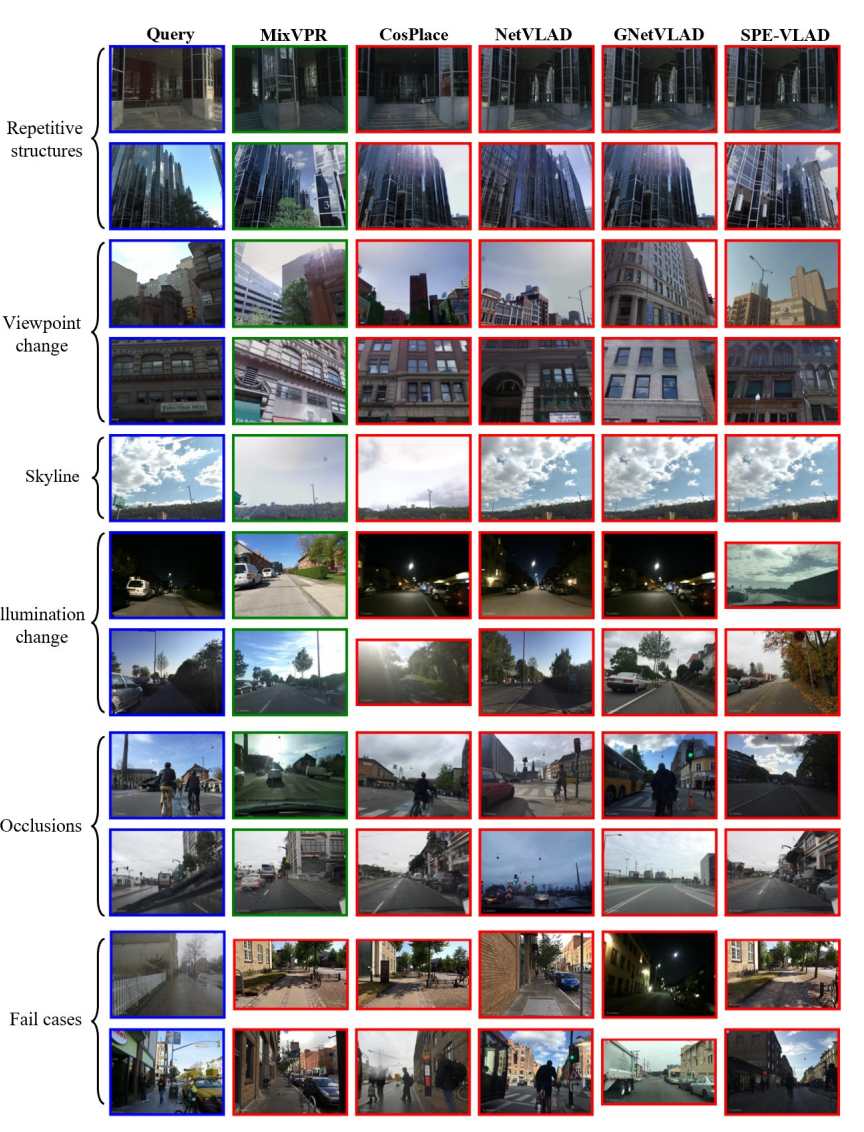
\includegraphics[width=\textwidth]{pics/Proposal/fail.png}
    \caption{Kết quả của những trường hợp khó khi chạy trên MixVPR và các phương pháp khác \cite{alibey2023mixvpr}}
\end{figure}

Với sự ra đời của AnyLoc \cite{keetha2023anyloc}, bài toán VPR trong những môi trường đa dạng hơn như trong nhà, trong hang động, trên bầu trời, hoặc trên mặt biển đã có một SOTA mới. Điều này là nhờ việc AnyLoc sử dụng mạng cơ sở DINO, một mạng Vision Transformer được huấn luyện bằng cơ chế tự giám sát để sinh ra những đặc trưng có giá trị với mọi tác vụ. Tuy nhiên, khi xét đến môi trường thành thị thì MixVPR vẫn có cho ra kết quả chính xác hơn AnyLoc. Số liệu cụ thể được trình bày bên dưới.

% \begin{figure}[H]
%   \centering
%   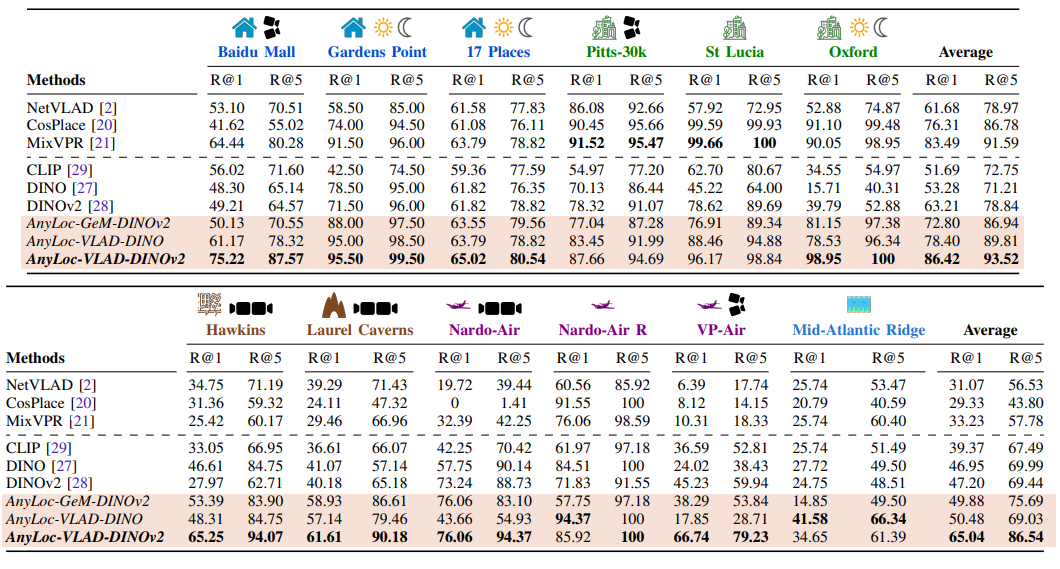
\includegraphics[scale=0.5]{pics/Proposal/anyloc.png}
%   \caption{Kết quả của AnyLoc so sánh với những mô hình khác \cite{keetha2023anyloc}}
% \end{figure}


\begin{table}[H]
    \adjustbox{max width=\textwidth}{
        \begin{tabular}{lcccccccccccccc}
            \cline{2-15}
            \multicolumn{1}{l|}{}                  & \multicolumn{2}{c|}{{\color[HTML]{6434FC} \textbf{Baidu Mall}}} & \multicolumn{2}{c|}{{\color[HTML]{6434FC} \textbf{Gardens Point}}} & \multicolumn{2}{c|}{{\color[HTML]{6434FC} \textbf{17 Places}}} & \multicolumn{2}{c|}{{\color[HTML]{009901} \textbf{Pitts-30k}}} & \multicolumn{2}{c|}{{\color[HTML]{009901} \textbf{St Lucia}}} & \multicolumn{2}{c|}{{\color[HTML]{009901} \textbf{Oxford}}} & \multicolumn{2}{c|}{\textbf{Average}}                                                                                                                                                                                              \\ \hline
            \multicolumn{1}{|l|}{\textbf{Methods}} & \multicolumn{1}{c|}{R@1}                                        & \multicolumn{1}{c|}{R@5}                                           & \multicolumn{1}{c|}{R@1}                                       & \multicolumn{1}{c|}{R@5}                                       & \multicolumn{1}{c|}{R@1}                                      & \multicolumn{1}{c|}{R@5}                                    & \multicolumn{1}{c|}{R@1}              & \multicolumn{1}{c|}{R@5} & \multicolumn{1}{c|}{R@1} & \multicolumn{1}{c|}{R@5} & \multicolumn{1}{c|}{R@1} & \multicolumn{1}{c|}{R@5} & \multicolumn{1}{c|}{R@1} & \multicolumn{1}{c|}{R@5} \\ \hline
            NetVLAD                                & 53.10                                                           & 70.51                                                              & 58.50                                                          & 85.00                                                          & 61.58                                                         & 77.83                                                       & 86.08                                 & 92.66                    & 57.92                    & 72.95                    & 52.88                    & 74.87                    & 61.68                    & 78.97                    \\
            CosPlace                               & 41.62                                                           & 55.02                                                              & 74.00                                                          & 94.50                                                          & 61.08                                                         & 76.11                                                       & 90.45                                 & 95.66                    & 99.59                    & 99.93                    & 91.10                    & 99.48                    & 76.31                    & 86.78                    \\
            MixVPR                                 & 64.44                                                           & 80.28                                                              & 91.50                                                          & 96.00                                                          & 63.79                                                         & 78.82                                                       & \textbf{91.52}                        & \textbf{95.47}           & \textbf{99.66}           & \textbf{100}             & 90.05                    & 98.95                    & 83.49                    & 91.59                    \\ \hline
            CLIP                                   & 56.02                                                           & 71.60                                                              & 42.50                                                          & 74.50                                                          & 59.36                                                         & 77.59                                                       & 54.97                                 & 77.20                    & 62.70                    & 80.67                    & 34.55                    & 54.97                    & 51.69                    & 72.75                    \\
            DINO                                   & 48.30                                                           & 65.14                                                              & 78.50                                                          & 95.00                                                          & 61.82                                                         & 76.35                                                       & 70.13                                 & 86.44                    & 45.22                    & 64.00                    & 15.71                    & 40.31                    & 53.28                    & 71.21                    \\
            DINOv2                                 & 49.21                                                           & 64.57                                                              & 71.50                                                          & 96.00                                                          & 61.82                                                         & 78.82                                                       & 78.32                                 & 91.07                    & 78.62                    & 89.69                    & 39.79                    & 52.88                    & 63.21                    & 78.84                    \\
            \rowcolor[HTML]{FFCE93}
            \textit{AnyLoc-GeM-DINOv2}             & 50.13                                                           & 70.55                                                              & 88.00                                                          & 97.50                                                          & 63.55                                                         & 79.56                                                       & 77.04                                 & 87.28                    & 76.91                    & 89.34                    & 81.15                    & 97.38                    & 72.80                    & 86.94                    \\
            \rowcolor[HTML]{FFCE93}
            \textit{AnyLoc-VLAD-DINO}              & 61.17                                                           & 78.32                                                              & 95.00                                                          & 98.50                                                          & 63.79                                                         & 78.82                                                       & 83.45                                 & 91.99                    & 88.46                    & 94.88                    & 78.53                    & 96.34                    & 78.40                    & 89.81                    \\
            \rowcolor[HTML]{FFCE93}
            \textit{\textbf{AnyLoc-VLAD-DINOv2}}   & \textbf{75.22}                                                  & \textbf{87.57}                                                     & \textbf{95.50}                                                 & \textbf{99.50}                                                 & \textbf{65.02}                                                & \textbf{80.54}                                              & 87.66                                 & 94.69                    & 96.17                    & 98.84                    & \textbf{98.95}           & \textbf{100}             & \textbf{86.42}           & \textbf{93.52}
        \end{tabular}}
    \caption{Bảng so sánh kết quả AnyLoc với những mô hình khác trên những tập dữ liệu thành thị}
\end{table}

\begin{table}[H]
    \adjustbox{max width=\textwidth}{
        \begin{tabular}{lcccccccccccccc}
            \cline{2-15}
            \multicolumn{1}{l|}{}                  & \multicolumn{2}{c|}{{\color[HTML]{986536} \textbf{Hawkins}}} & \multicolumn{2}{c|}{{\color[HTML]{986536} \textbf{Laurel Caverns}}} & \multicolumn{2}{c|}{{\color[HTML]{6200C9} \textbf{Nardo-Air}}} & \multicolumn{2}{c|}{{\color[HTML]{6200C9} \textbf{Nardo-Air R}}} & \multicolumn{2}{c|}{{\color[HTML]{6200C9} \textbf{VP-Air}}} & \multicolumn{2}{c|}{{\color[HTML]{3531FF} \textbf{\begin{tabular}[c]{@{}c@{}}Mid-Atlantic\\ Ridge\end{tabular}}}} & \multicolumn{2}{c|}{\textbf{Average}}                                                                                                                                                                                              \\ \hline
            \multicolumn{1}{|l|}{\textbf{Methods}} & \multicolumn{1}{c|}{R@1}                                     & \multicolumn{1}{c|}{R@5}                                            & \multicolumn{1}{c|}{R@1}                                       & \multicolumn{1}{c|}{R@5}                                         & \multicolumn{1}{c|}{R@1}                                    & \multicolumn{1}{c|}{R@5}                                                                                          & \multicolumn{1}{c|}{R@1}              & \multicolumn{1}{c|}{R@5} & \multicolumn{1}{c|}{R@1} & \multicolumn{1}{c|}{R@5} & \multicolumn{1}{c|}{R@1} & \multicolumn{1}{c|}{R@5} & \multicolumn{1}{c|}{R@1} & \multicolumn{1}{c|}{R@5} \\ \hline
            NetVLAD                                & 34.75                                                        & 71.19                                                               & 39.29                                                          & 71.43                                                            & 19.72                                                       & 39.44                                                                                                             & 60.56                                 & 85.92                    & 6.39                     & 17.74                    & 25.74                    & 53.47                    & 31.07                    & 56.53                    \\
            CosPlace                               & 31.36                                                        & 59.32                                                               & 24.11                                                          & 47.32                                                            & 0                                                           & 1.41                                                                                                              & 91.55                                 & \textbf{100}             & 8.12                     & 14.15                    & 20.79                    & 40.59                    & 29.33                    & 43.80                    \\
            MixVPR                                 & 25.42                                                        & 60.17                                                               & 29.46                                                          & 66.96                                                            & 32.39                                                       & 42.25                                                                                                             & 76.06                                 & 98.59                    & 10.31                    & 18.33                    & 25.74                    & 60.40                    & 33.23                    & 57.78                    \\ \hline
            CLIP                                   & 33.05                                                        & 66.95                                                               & 36.61                                                          & 66.07                                                            & 42.25                                                       & 70.42                                                                                                             & 61.97                                 & 97.18                    & 36.59                    & 52.81                    & 25.74                    & 51.49                    & 39.37                    & 67.49                    \\
            DINO                                   & 46.61                                                        & 84.75                                                               & 41.07                                                          & 57.14                                                            & 57.75                                                       & 90.14                                                                                                             & 84.51                                 & 100                      & 24.02                    & 38.43                    & 27.72                    & 49.50                    & 46.95                    & 69.99                    \\
            DINOv2                                 & 27.97                                                        & 62.71                                                               & 40.18                                                          & 65.18                                                            & 73.24                                                       & 88.73                                                                                                             & 71.83                                 & 91.55                    & 45.23                    & 59.94                    & 24.75                    & 48.51                    & 47.20                    & 69.44                    \\
            \rowcolor[HTML]{FFCE93}
            \textit{AnyLoc-GeM-DINOv2}             & 53.39                                                        & 83.90                                                               & 58.93                                                          & 86.61                                                            & 76.06                                                       & 83.10                                                                                                             & 57.75                                 & 97.18                    & 38.29                    & 53.84                    & 14.85                    & 49.50                    & 49.88                    & 75.69                    \\
            \rowcolor[HTML]{FFCE93}
            \textit{AnyLoc-VLAD-DINO}              & 48.31                                                        & 84.75                                                               & 57.14                                                          & 79.46                                                            & 43.66                                                       & 54.93                                                                                                             & \textbf{94.37}                        & \textbf{100}             & 17.85                    & 28.71                    & \textbf{41.58}           & \textbf{66.34}           & 50.48                    & 69.03                    \\
            \rowcolor[HTML]{FFCE93}
            \textit{\textbf{AnyLoc-VLAD-DINOv2}}   & \textbf{65.25}                                               & \textbf{94.07}                                                      & \textbf{61.61}                                                 & \textbf{90.18}                                                   & \textbf{76.06}                                              & \textbf{94.37}                                                                                                    & 85.92                                 & \textbf{100}             & \textbf{66.74}           & \textbf{79.23}           & 34.65                    & 61.39                    & \textbf{65.04}           & \textbf{86.54}
        \end{tabular}}
    \caption{Bảng so sánh kết quả AnyLoc với những mô hình khác trên những tập dữ liệu ngoài thiên nhiên}
\end{table}
\section{Module hồi quy tư thế tương đối - RPR}
Mô hình tương quan 2D-2D được đề xuất trong Map-free Relocalization \cite{arnold2022mapfree} thuộc nhóm những phương pháp định vị theo hướng tiếp cận truyền thống sử dụng Essential Matrix. So với những phương pháp RPR thường thấy, phương pháp này giải quyết được vấn đề không nắm bắt được thông tin về hình học trong ảnh. Mô hình vẫn đạt được kết quả cạnh tranh trong những môi trường có mật độ ảnh dày đặc. Tuy nhiên, khi được đưa vào môi trường mà ảnh tham khảo và ảnh truy vấn xa nhau hơn thì phương pháp này lại có kết quả vượt trội hơn hẳn những phương pháp khác. Mô hình tương quan 2D-2D xác định Essential Matrix giữa 2 ảnh thông qua những cặp điểm tương quan, từ đó tính toán được khác biệt về hướng lệch vị trí và góc quay. Sử dụng thêm thông tin về độ sâu, mô hình xác định được khoảng cách cách biệt thực giữa cặp ảnh và qua đó có được vị trí thực của ảnh truy vấn.

\subsection{Kiến trúc}

\begin{figure}[htbp]
  \centering
  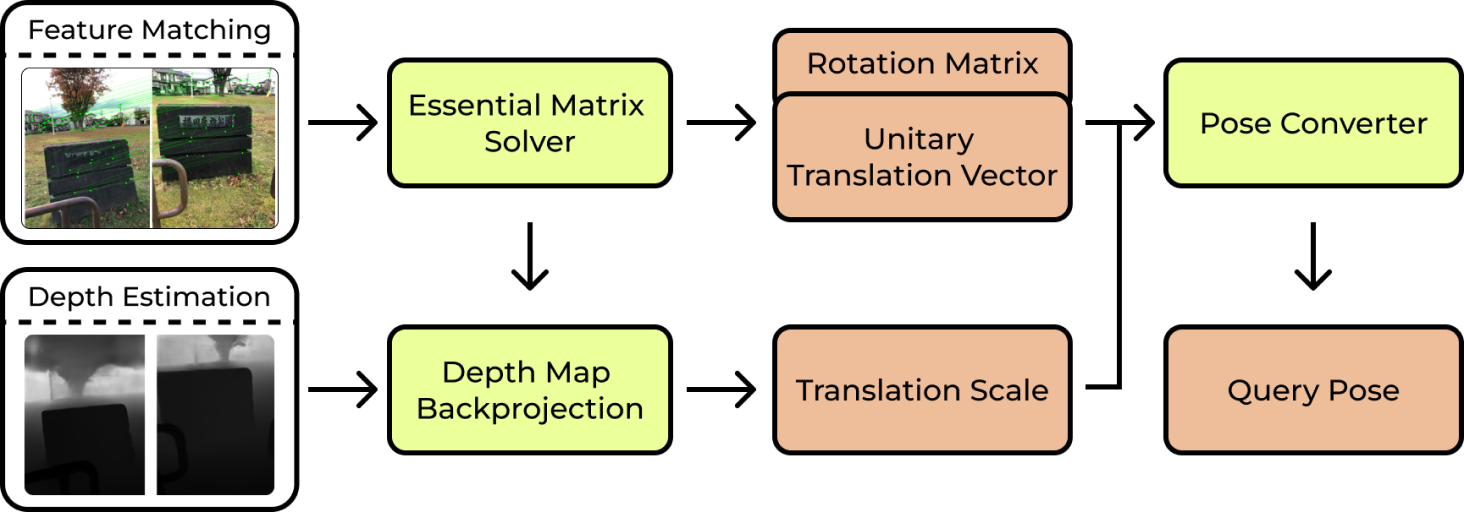
\includegraphics[width=\textwidth]{pics/Proposal/2d_2d.png}
  % \includesvg[scale=0.3]{pics/Proposal/arch.svg}
  \caption{Kiến trúc tổng quan của mô hình tương quan 2D-2D}
\end{figure}

\subsubsection{Mô hình xác định cặp đặc trưng và ước tính độ sâu của ảnh}

Với dữ liệu đầu vào là cặp ảnh gồm ảnh truy vấn và ảnh tham khảo $(I, I_0)$, tại bước này, những cặp đặc trưng tương quan sẽ được xác định và vị trí của chúng sẽ được lưu lại trong 2 tập là $(kpts_0, ktps_1)$. Mô hình ghép đặc trưng được sử dụng sẽ là SuperPoint+SuperGlue \cite{sarlin2020superglue} đã trải qua quá trình huấn luyện. Bản đồ thông tin độ sâu của mỗi ảnh cũng sẽ được sinh ra bằng mô hình DPT \cite{ranftl2021vision} được huấn luyện trên tập KITTI do phạm vi được sử dụng của mô hình sẽ là ở ngoài trời, trong khu vực thành thị \cite{arnold2022mapfree}. Dữ liệu trả về của 2 mô hình này sẽ là hai tập chứa vị trí của các điểm đặc trưng tương ứng và bản đồ độ sâu ước tính của mỗi hình.

\begin{figure}[H]
  \centering
  \begin{minipage}[b]{0.48\textwidth}
    \captionsetup{justification=centering}
    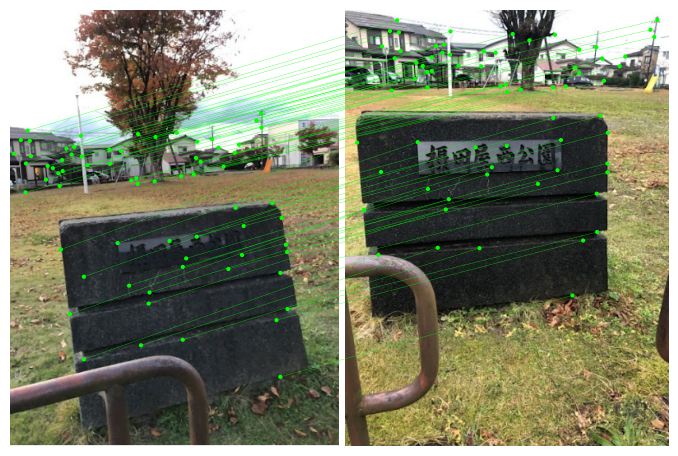
\includegraphics[width=\textwidth]{pics/Proposal/matching.png}
    \caption{Kết quả của quá trình xác định và ghép đặc trưng}
  \end{minipage}
  \begin{minipage}[b]{0.48\textwidth}
    \captionsetup{justification=centering}
    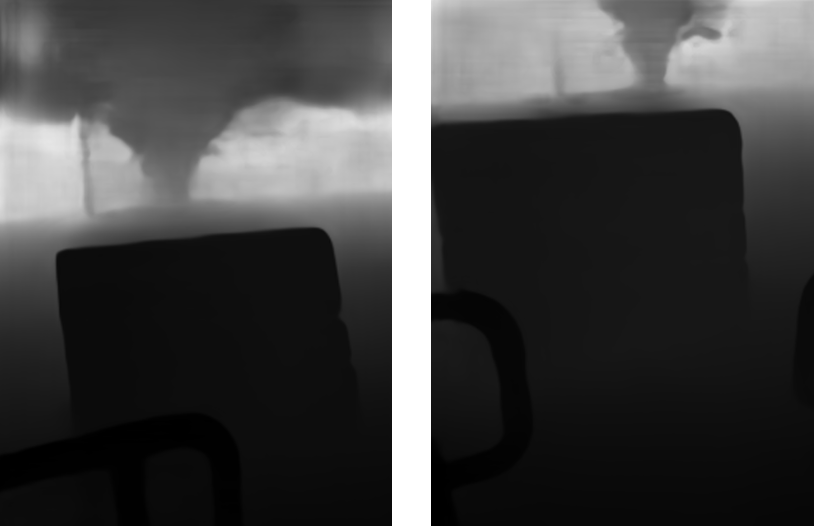
\includegraphics[width=\textwidth]{pics/Proposal/depth.png}
    \caption{Kết quả của quá trình ước tính độ sâu ảnh}
  \end{minipage}
  % \begin{minipage}[t]{0.3\textwidth}
  %     \caption{Kết quả của quá trình xác định và ghép đặc trưng}
  % \end{minipage}
  % \begin{minipage}[t]{0.3\textwidth}
  %     \caption{Kết quả của quá trình ước tính độ sâu ảnh}
  % \end{minipage}
\end{figure}

\subsubsection{Bộ phận khai phá Essential Matrix}

Dựa vào những cặp đặc trưng tương quan đã được xác định trong các tập $(kpts_0, kpts_1)$ và ma trận thông số $T_0, T_1$ của camera của mỗi ảnh, Essential Matrix $M$ được ước tính dựa vào giải thuật 5 điểm \cite{nister2004efficient} cùng với vòng lặp MAGSAC++ \cite{barath2020magsac++}. Ma trận thông số $T_i$ của camera sẽ chứa các thông tin về tiêu cự của camera $f_x,f_y$ và tọa độ điểm chính của camera $c_x,c_y$, được sắp xếp thành ma trận như sau:
\begin{equation}
  T_i = \begin{bmatrix} f_x & 0 & c_x \\ 0 & f_y & c_y \\ 0 & 0 & 1 \end{bmatrix}
\end{equation}
Essential Matrix $M$ sau đó sẽ được phân giải thành ma trận thể hiện góc quay chênh lệch, $R \in SO(3)$ và vector đơn vị độ lệch về vị trí giữa hai ảnh, $\hat{t} \in R^{3}, \lvert \hat{t} \rvert = 1$. Tập những cặp điểm tương quan thỏa Essential Matrix $M$ cũng sẽ được trả về.

\subsubsection{Bộ phận chiếu cặp điểm tương quan lên không gian ba chiều}

Những cặp điểm tương quan (inlier correspondence) thỏa ma trận $M$ sau đó sẽ được chiếu lên không gian 3D qua bản đồ độ sâu ảnh đã được sinh ra ở mỗi ảnh. Với mỗi cặp điểm $p_0, p_1$ đã được chiếu lên không gian 3D, mô hình sẽ tìm được một giá trị tỷ lệ $s^*$ cho $\hat{t}$ để làm giảm thiểu độ lệch của điểm $p_0$ khi được chiếu lên hệ tọa độ của camera thứ hai và điểm $p_1$. Giá trị $s$ tương ứng với mỗi cặp điểm $(p_0, p_1)$ có thể được xác định qua công thức:

\begin{equation}
  \begin{aligned}
    s=\underset{s^*}{\arg \min }\left\|R p_A+s^* \cdot \hat{t}-p_B\right\|_2 .
  \end{aligned}
\end{equation}

\begin{figure}[H]
  \centering
  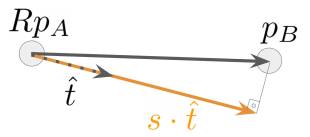
\includegraphics[scale=1]{pics/Proposal/reprojection.png}
  \caption[Minh họa cho việc xác định tỷ lệ $s$ bằng độ sâu ảnh]{Hình minh họa cho việc chiếu điểm $p_0$ qua vector góc quay $R$ và vector độ lệch đơn vị $\hat{t}$ cùng với tỷ lệ $s$ để tối thiểu khoảng cách \cite{arnold2022mapfree}}
\end{figure}

Cuối cùng, tỷ lệ $s^*$ với số cặp điểm hợp lệ cao nhất sẽ được chọn làm kết quả cuối cùng. Một cặp điểm sẽ được xem như hợp lệ khi khoảng cách sai lệch giữa hai điểm 3D sau khi chiếu nhỏ hơn một ngưỡng nhất định, ở đây được xác định là 10cm. Vòng lặp RANSAC sẽ được sử dụng để bỏ những trường hợp ngoại lệ.

Sau khi chạy qua những bước trên, mô hình sẽ thu về được các giá trị thể hiện độ lệch giữa vị trí và góc quay của cặp ảnh truy vấn và tham khảo dưới dạng ma trận độ lệch góc quay $R$ và vector độ lệch vị trí $s*\hat{t}$. Ma trận độ lệch góc quay $R$ sau đó sẽ được phân giải thành một Quaternion - được biểu diễn dưới dạng một tập 4 số là $q^{\Delta} = (q^{\Delta}_w,q^{\Delta}_x,q^{\Delta}_y,q^{\Delta}_z)$ - thể hiện góc quay trong không gian. Vector độ lệch vị trí sẽ có dạng bộ 3 số là $(t^{\Delta} = t^{\Delta}_x,t^{\Delta}_y,t^{\Delta}_z)$. Ngoài ra, số cặp điểm tương quan có độ lệch dưới 10cm với giá trị $s^*$ được chọn sẽ được dùng làm thông số đánh giá độ đáng tin cậy $C$ của dự đoán.


\subsubsection{Bộ phận tính toán tư thế tuyệt đối}

Từ kết quả của những bộ phận trên, mô hình đã biểu diễn được góc quay và vị trí tương đối giữa hai ảnh $(q^{\Delta},t^{\Delta})$. Khi biết được tọa độ chính xác của ảnh tham khảo $(q^{ref},t^{ref})$, mô hình sẽ tính được tọa độ và góc quay chính xác của ảnh truy vấn và đưa ra kết quả cuối cùng là hai tập $(q^{abs},t^{abs})$

Để xác định được góc quay chính xác của ảnh truy vấn, mô hình biến đổi góc quay của ảnh tham khảo với độ lệch góc quay đã xác định được giữa hai ảnh theo công thức:

\begin{equation}
  \begin{aligned}
    q^{abs}                                   & = q^{\Delta} * q^{ref}                                                                                    \\
    (q^{abs}_w,q^{abs}_x,q^{abs}_y,q^{abs}_z) & = (q^{\Delta}_w,q^{\Delta}_x,q^{\Delta}_y,q^{\Delta}_z) * (q^{ref}_w,q^{ref}_x,q^{ref}_y,q^{ref}_z)       \\ \\
    q^{abs}_w                                 & =\left(q^{\Delta}_w q^{ref}_w-q^{\Delta}_x q^{ref}_x-q^{\Delta}_y q^{ref}_y-q^{\Delta}_z q^{ref}_z\right) \\
    q^{abs}_x                                 & =\left(q^{\Delta}_w q^{ref}_x+q^{\Delta}_x q^{ref}_w-q^{\Delta}_y q^{ref}_z+q^{\Delta}_z q^{ref}_y\right) \\
    q^{abs}_y                                 & =\left(q^{\Delta}_w q^{ref}_y+q^{\Delta}_x q^{ref}_z+q^{\Delta}_y q^{ref}_w-q^{\Delta}_z q^{ref}_x\right) \\
    q^{abs}_z                                 & =\left(q^{\Delta}_w q^{ref}_z-q^{\Delta}_x q^{ref}_y+q^{\Delta}_y q^{ref}_x+q^{\Delta}_z q^{ref}_w\right)
  \end{aligned}
\end{equation}

Để xác định vị trí chính xác của ảnh truy vấn trong không gian thực, vị trí kinh độ, vĩ độ và độ cao của ảnh chụp có thể được xác định qua công thức:

\begin{equation}
  \begin{aligned}
    t^{abs}                         & = t^{\Delta} + t^{ref}                                                       \\
    (t^{abs}_x,t^{abs}_y,t^{abs}_z) & = (t^{\Delta}_x,t^{\Delta}_y,t^{\Delta}_z) + (t^{ref}_x,t^{ref}_y,t^{ref}_z) \\ \\
    t^{abs}_x                       & = t^{\Delta}_x + t^{ref}_x                                                   \\
    t^{abs}_y                       & = t^{\Delta}_y + t^{ref}_y                                                   \\
    t^{abs}_z                       & = t^{\Delta}_z + t^{ref}_z                                                   \\
  \end{aligned}
\end{equation}

\subsection{Phương pháp hiện thực và triển khai}
\subsubsection{Hiện thực}
Tác vụ tìm kiếm tương quan giữa hai ảnh có thể lựa chọn giữa các phương pháp truyền thống như SIFT, hoặc những phương pháp theo hướng tiếp cận học sâu gần đây như SuperPoint+SuperGlue \cite{sarlin2020superglue} và LoFTR \cite{sun2021loftr}. Tác vụ tính độ sâu đơn ảnh sẽ được phân thành hai trường hợp là bên trong nhà và ngoài trời. Với những tập dữ liệu trong nhà, mô hình DPT \cite{ranftl2021vision} được huấn luyện trên tập dữ liệu NYUv2 \cite{silberman2012indoor} PlaneRCNN \cite{liu2019planercnn} được huấn luyện trên tập dữ liệu ScanNet \cite{dai2017scannet}. Với trường hợp ngoài trời, mô hình DPT \cite{ranftl2021vision} được huấn luyện trên tập KITTI sẽ được sử dụng \cite{geiger2012we}. Mô hình SuperPoint+SuperGlue sẽ được chọn để thực hiện tác vụ Feature Matching và mô hình DPT được huấn luyện trên tập KITTI sẽ được dùng để thực hiện tác vụ Monocular Depth Estimation, nhờ vào độ chính xác cao thể hiện trong \cite{arnold2022mapfree}.

\subsubsection{Phương pháp đánh giá}
Để đánh giá hiệu quả của mô hình trong tác vụ định vị trực quan, một số tiêu chí cơ bản đã được đưa ra như độ lệch về góc quay, độ lệch về vị trí của camera, cũng như một sai số mới được đưa ra trong bài nghiên cứu, sai số phản chiếu của điểm 3D ảo - VCRE, được lấy cảm hứng từ sai số phản chiếu của những điểm tương ứng - DCRE \cite{wald2020beyond}. Cụ thể, với giá trị dự đoán $(R,t)$ và giá trị thực $(R_{gt},t_{gt})$, các sai số sẽ được xác định như sau:
\begin{itemize}
  \item Sai số về góc quay, $\measuredangle(R,R_{gt})$, sẽ được tính là độ chênh lệch giữa góc quay được dự đoán và góc quay thực tế.
  \item Sai số về độ lệch vị trí máy quay sẽ được tính là khoảng cách Euclidean giữa cặp vị trí $(t,t_{gt})$ được tính theo công thức $c=-R \intercal t$.
  \item Sai số phản chiếu của điểm 3D ảo sẽ được dùng để đánh giá độ lệch của những vật thể trong không gian thực tế ảo. Giá trị thực $(R_{gt},t_{gt})$ và giá trị dự đoán $(R,t)$ sẽ được dùng để chiếu những điểm 3D ảo, lên hệ tọa độ của camera truy vấn. Giá trị VCRE sẽ được xác định theo công thức
        \begin{equation}
          \operatorname{VCRE}=\frac{1}{|\mathcal{V}|} \sum_{\mathbf{v} \in \mathcal{V}}\left\|\pi(\mathbf{v})-\pi\left(T T_{\mathrm{gt}}^{-1} \mathbf{v}\right)\right\|_2 \quad \text { với } T=[R \mid t]
        \end{equation}

        với $\pi$ là phép chiếu từ không gian camera lên ảnh, $\mathcal{V}$ là một tập các điểm 3D, đại diện cho những vật thể ảo. $\mathcal{V}$ là một lưới điểm 3D, (chiều cao là 4, chiều rộng là 7 và chiều sâu là 7), cách nhau 30cm và có độ dịch là 1.8m dọc theo trục của máy ảnh. Giá trị sai số của phép phản chiếu sẽ được so sánh với đường chéo của ảnh.
  \item Độ tin cậy $C$ của dự đoán cũng là một tiêu chí được đánh giá. Giá trị này cho phép mô hình có thể phát hiện và loại bỏ những dự đoán không đáng tin cậy. Giá trị này sẽ được xác định bằng số lượng cặp điểm tương quan thỏa Essential Matrix được chọn trên tổng số cặp điểm tương quan xác định bởi mô hình ghép đặc trưng. Với một ngưỡng tin cậy nhất định, tỷ lệ dự đoán đáng tin cậy - ratio of confident estimate, sẽ được xác định là tỷ lệ ảnh truy vấn có độ tin cậy vượt qua ngưỡng.
  \item Độ chính xác của mô hình sẽ là tỷ lệ ảnh đáng tin cậy có sai lệch giữa giá trị dự đoán và giá trị thực dưới một ngưỡng nhất định (độ lệch vị trí và góc quay) hoặc có sai số phản chiếu chấp nhận được trên tổng số ảnh.
\end{itemize}

Tập dữ liệu 7Scenes \cite{6619221} được sử dụng để xác định hiệu suất mô hình tiêu chuẩn của Map-free so với những phương pháp SOTA tại thời điểm đó, với số lượng ảnh tham khảo là rất nhiều. Ảnh hưởng của việc giảm số lượng ảnh tham khảo lên khả năng hoạt động của các mô hình cũng sẽ được ghi nhận lại. Tập dữ liệu Niantic \cite{arnold2022mapfree} được đề xuất trong cùng bài nghiên cứu cũng sẽ được sử dụng để đánh giá, nhằm xác định hiệu suất của các mô hình trong trường hợp chỉ có một ảnh tham khảo.


\subsection{Kết quả}
\subsubsection{Tập dữ liệu 7Scenes}

\begin{table}[H]
  \adjustbox{max width=\textwidth}{
    \begin{tabular}{|c|r|c|c|}
      \hline
      \multicolumn{1}{|l|}{\textbf{}}                                                                  & \textbf{Method}                                                                      & \textbf{\begin{tabular}[c]{@{}c@{}}Average Median\\ Pose Error\end{tabular}} & \textbf{\begin{tabular}[c]{@{}c@{}}Precision @ VCRE\\ 5\% / 10\% diag\end{tabular}} \\ \hline
                                                                                                       & \cellcolor[HTML]{C5FFD9}DSAC*                                                        & \cellcolor[HTML]{C5FFD9}3 cm, 1.1°                                           & \cellcolor[HTML]{C5FFD9}0.98/0.99                                                   \\
                                                                                                       & \cellcolor[HTML]{C5FFD9}hLoc                                                         & \cellcolor[HTML]{C5FFD9}3 cm, 1.0°                                           & \cellcolor[HTML]{C5FFD9}N/A                                                         \\
      \multirow{-3}{*}{\textbf{\begin{tabular}[c]{@{}c@{}}Structure\\ -based\end{tabular}}}            & \cellcolor[HTML]{C5FFD9}ActiveSearch                                                 & \cellcolor[HTML]{C5FFD9}4 cm, 1.2°                                           & \cellcolor[HTML]{C5FFD9}N/A                                                         \\ \hline
                                                                                                       & \cellcolor[HTML]{C5FFD9}EssNet (Ess.Mat.)                                            & \cellcolor[HTML]{C5FFD9}22 cm, 8.0°                                          & \cellcolor[HTML]{C5FFD9}N/A                                                         \\
                                                                                                       & \cellcolor[HTML]{F8BA5D}ExReNet                                                      & \cellcolor[HTML]{F8BA5D}9 cm, 2.7°                                           & \cellcolor[HTML]{F8BA5D}N/A                                                         \\
                                                                                                       & \cellcolor[HTML]{ECF4FF}ExReNet                                                      & \cellcolor[HTML]{ECF4FF}12 cm, 3.3°                                          & \cellcolor[HTML]{ECF4FF}N/A                                                         \\
                                                                                                       & \cellcolor[HTML]{ECF4FF}SIFT (Ess.Mat.)                                              & \cellcolor[HTML]{ECF4FF}8 cm, 2.0°                                           & \cellcolor[HTML]{ECF4FF}0.87/0.93                                                   \\
      \multirow{-5}{*}{\textbf{\begin{tabular}[c]{@{}c@{}}Pose\\ Triangulation\end{tabular}}}          & \cellcolor[HTML]{ECF4FF}SuperGlue (Ess.Mat.)                                         & \cellcolor[HTML]{ECF4FF}7 cm, 1.5°                                           & \cellcolor[HTML]{ECF4FF}0.93/0.97                                                   \\ \hline
                                                                                                       & \cellcolor[HTML]{ECF4FF}RelocNet                                                     & \cellcolor[HTML]{ECF4FF}29 cm, 11.3°                                         & \cellcolor[HTML]{ECF4FF}N/A                                                         \\
                                                                                                       & \cellcolor[HTML]{ECF4FF}RPR {[}R($\alpha$,$\beta$,$\gamma$)+s.t($\theta$, $\phi$){]} & \cellcolor[HTML]{ECF4FF}18 cm, 4.9°                                          & \cellcolor[HTML]{ECF4FF}0.71/0.93                                                   \\
      \multirow{-3}{*}{\textbf{RPR}}                                                                   & \cellcolor[HTML]{ECF4FF}RPR {[}3D-3D{]}                                              & \cellcolor[HTML]{ECF4FF}16 cm, 4.5°                                          & \cellcolor[HTML]{ECF4FF}0.82/0.96                                                   \\ \hline
                                                                                                       & \cellcolor[HTML]{ECF4FF}SIFT (Ess.Mat.+D.Scale)                                      & \cellcolor[HTML]{ECF4FF}16 cm, 2.5°                                          & \cellcolor[HTML]{ECF4FF}0.84/0.94                                                   \\
                                                                                                       & \cellcolor[HTML]{ECF4FF}SuperGlue (Ess.Mat.+D.Scale)                                 & \cellcolor[HTML]{ECF4FF}13 cm, 1.8°                                          & \cellcolor[HTML]{ECF4FF}0.89/0.97                                                   \\
                                                                                                       & \cellcolor[HTML]{ECF4FF}SIFT (PnP)                                                   & \cellcolor[HTML]{ECF4FF}12 cm, 3.3°                                          & \cellcolor[HTML]{ECF4FF}0.89/0.95                                                   \\
      \multirow{-4}{*}{\textbf{\begin{tabular}[c]{@{}c@{}}Feat.matching\\ + Depth Scale\end{tabular}}} & \cellcolor[HTML]{ECF4FF}SuperGlue (PnP)                                              & \cellcolor[HTML]{ECF4FF}10 cm, 2.8°                                          & \cellcolor[HTML]{ECF4FF}0.92/0.98                                                   \\ \hline
    \end{tabular}}
  \caption[Bảng so sánh hiệu quả của các mô hình trên tập dữ liệu 7Scenes]{Hiệu quả của những mô hình khi có đầy đủ ảnh tham khảo trên tập 7Scenes. Những phương pháp \textcolor{green}{xanh lá} sẽ phụ thuộc vào tập dữ liệu, phương pháp \textcolor{orange}{cam} được huấn luyện trên SUNCG \cite{song2017semantic} và \textcolor{blue}{xanh dương} trên tập ScanNet \cite{dai2017scannet}}
\end{table}

Khi xét trên tập dữ liệu 7Scenes với tất cả các ảnh tham khảo, những phương pháp sử dụng biểu diễn 3D như DSAC* \cite{brachmann2021visual}, hLoc \cite{sarlin2019coarse}, ActiveSearch \cite{sattler2016efficient} có kết quả tốt nhất, tuy nhiên lại phụ thuộc vào quá trình tái tạo lại cấu trúc. Những phương pháp sử dụng phép đạc tam giác - Triangulation, sử dụng 5 ảnh tham khảo có kết quả cạnh tranh so với những phương pháp sử dụng biểu diễn 3D, được ký hiệu bằng $\triangle$. Những phương pháp trong tập \textit{RPR End-to-End} và \textit{Feat.Matching - Depth Scale} chỉ sử dụng một ảnh tham khảo để truy vấn. Cả hai lớp phương pháp đều có kết quả không chính xác bằng những phương pháp biểu diễn 3D. Tuy nhiên, phương pháp Feat.Matching - Depth Scale có hiệu quả cao hơn những phương pháp RPR End-to-End.


\begin{figure}[H]
  \centering
  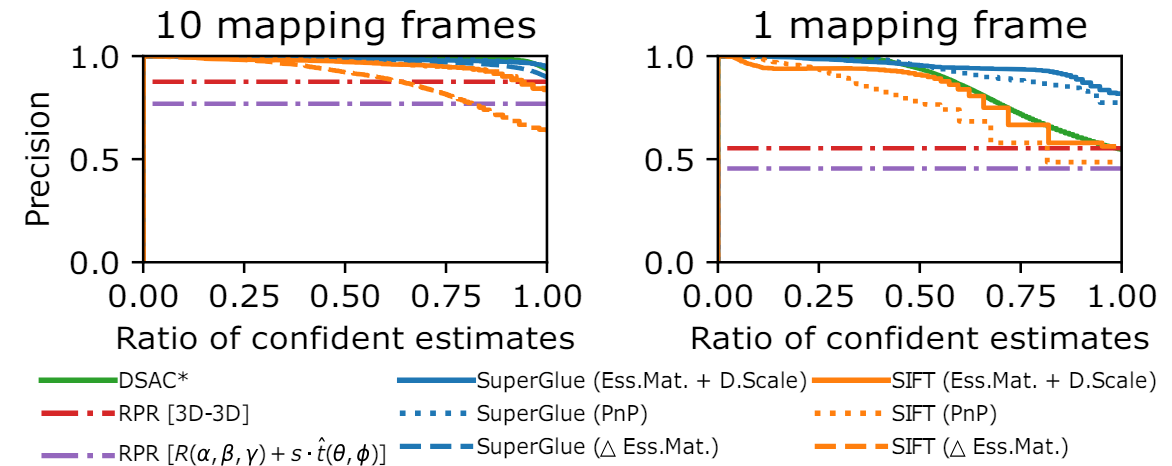
\includegraphics[width=0.6\textwidth]{pics/Proposal/partial_7scene.png}
  \caption[Hiệu quả của các mô hình khi giới hạn ảnh tham khảo]{Hiệu quả của những mô hình khi tập 7Scenes chỉ có 10/1 ảnh tham khảo, đánh giá về độ chính xác. Đối với những mô hình RPR không có phương pháp đánh giá về độ đáng tin cậy của dự đoán, một đường thẳng ngang sẽ được dùng để thể hiện độ chính xác}
\end{figure}

Để có thể phản ánh một môi trường thực tế, nơi mà ảnh tham khảo truy xuất được cách xa một khoảng đáng kể so với ảnh truy vấn, $K$ ảnh tham khảo mang nhiều thông tin nhất sẽ được chọn làm đại diện qua giải thuật gom cụm K-means.

Hai đồ thị trên thể hiện sự thay đổi về độ chính xác, những dự đoán có $VCRE<80px$ khi tỷ lệ kết quả chấp nhận thay đổi. Tỷ lệ số dự đoán chấp nhận sẽ tăng dần khi ngưỡng chấp nhận dần lỏng ra. Điều này đồng thời cũng làm cho độ chính xác cũng giảm dần do tăng khả năng những dự đoán không có cơ sở chắc chắn cũng được xem là đáng tin. Trong trường hợp này, những mô hình 2D-2D, đặc biệt là mô hình sử dụng SuperGlue, có kết quả tốt hơn so với những mô hình còn lại. Điều này thể hiện rõ nhất trong khoảng 0.5~1.0 ở cả 2 kịch bản $K=10$ và $K=1$.

Mô hình DSAC* vẫn có kết quả cạnh tranh. Tuy nhiên, phương pháp này lại quá phụ thuộc vào tập dữ liệu. Trong khi đó, những mô hình khác được huấn luyện trên tập ScanNet vẫn có kết quả tốt trên tập 7Scenes. Phương pháp sử dụng phép Triangulation cũng có kết quả cạnh tranh, tuy nhiên lại không thể hoạt động chỉ với một ảnh tham khảo. Những phương pháp Feat.Matching - Depth Scale có khả năng khái quát hóa tốt hơn những phương pháp RPR End-to-End, thể hiện qua hiệu quả tương đối tốt hơn.

\subsubsection{Tập dữ liệu Niantic}

\begin{figure}[H]
  \centering
  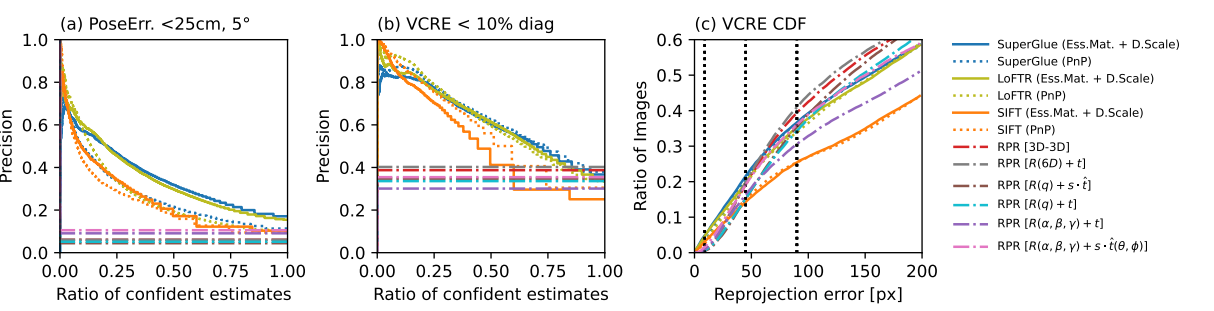
\includegraphics[width=\textwidth]{pics/Proposal/all_niantic.png}
  \caption{Hiệu quả của các mô hình trên tập dữ liệu Niantic, xác định theo độ chính xác và số ảnh có sai số phản chiếu dưới ngưỡng}
\end{figure}

Qua kết quả thu được, tập dữ liệu Niantic có độ khó cao hơn đáng kể so với tập dữ liệu 7Scenes với mọi phương pháp. Trong tập dữ liệu Niantic, những phương pháp Feat.Matching - Depth Scale tiếp tục có kết quả tốt. Tuy nhiên, ở những ngưỡng đáng tin cậy rộng hơn, những phương pháp RPR lại có kết quả tốt hơn. Điều này có thể giải thích được qua hiện tượng: khi số cặp đặc trưng tương quan là không đủ chất lượng, độ lệch đơn vị vị trí được sinh ra có sai số rất lớn so với thực tế ở những phương pháp Feat.Matching - Depth Scale. Những phương pháp RPR End-to-End cho ra kết quả tốt khi ngưỡng chính xác rộng, nhưng lại có kết quả không tốt khi cần độ chính xác cao. Ngoài ra, những phương pháp RPR End-to-End cũng không thể cung cấp độ tin cậy cho dự đoán của mô hình, không thể loại bỏ những dự đoán có khả năng sai cao.

\section{Đề xuất phát triển}

\subsection{Chiến lược khai phá đặc trưng dựa trên độ trùng lắp}
Ảnh tham khảo truy xuất được từ tác vụ VPR tiềm ẩn rủi ro không đủ độ trùng lắp với ảnh đầu vào, dẫn đến sai sót trong quá trình tính toán tư thế. Để giải quyết vấn đề này, chúng tôi đề xuất một chiến lược khai phá mới dựa trên hàm khai phá Multi-Similarity Miner \cite{wang2019multi} nhằm đảm bảo tính trùng lấp về vùng khung hình(frustum) cao giữa các ảnh. Điều này sẽ hỗ trợ cho quá trình Feature Matching tại module RPR ở phía sau.

Cụ thể hơn, chúng tôi xác định một cặp ảnh là được một positive pair nếu có độ trùng lắp frustum cao hơn một ngưỡng nhất định, tức giữa cặp ảnh chia sẻ nhiều điểm chung hơn. Để đảm bảo độ vững chắc của mô hình không bị tác động, chúng tôi sử dụng cơ chế trùng lắp camera frustum song phương từ \cite{9008579}, được tính bằng tổng độ trùng lắp frustum từ một ảnh đến ảnh còn lại và ngược lại.

Tuy nhiên, độ trùng lắp cao vẫn có thể xuất hiện trong trường hợp các ảnh được chụp ở hai góc độ hoàn toàn ngược nhau, gây nên khó khăn và sai lệch trong quá trình dự đoán tư thế tuyệt đối do góc quay khác biệt quá lớn. Để giải quyết vấn đề này, chúng tôi đặt ra điều kiện khác biệt hướng nhìn làm một tiêu chuẩn phụ trong việc chấp nhận các cặp ảnh. Cụ thể hơn, các cặp ảnh không được phép có hướng nhìn lệch nhau quá một tiêu chuẩn nhất định mà chúng tôi đặt ra.

% \begin{figure}
%   \centering
%   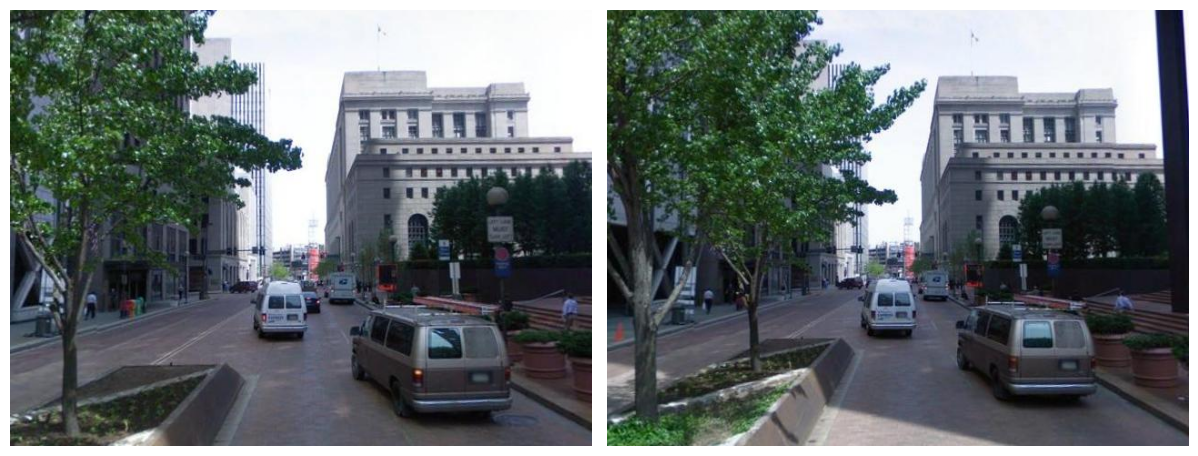
\includegraphics[width=\textwidth]{pics/Chapter3/highoverlap.png}
%   \caption[Cặp ảnh có độ overlap cao]{Cặp ảnh được chấp nhận - có độ trùng lắp cao}
% \end{figure}

% \begin{figure}
%   \centering
%   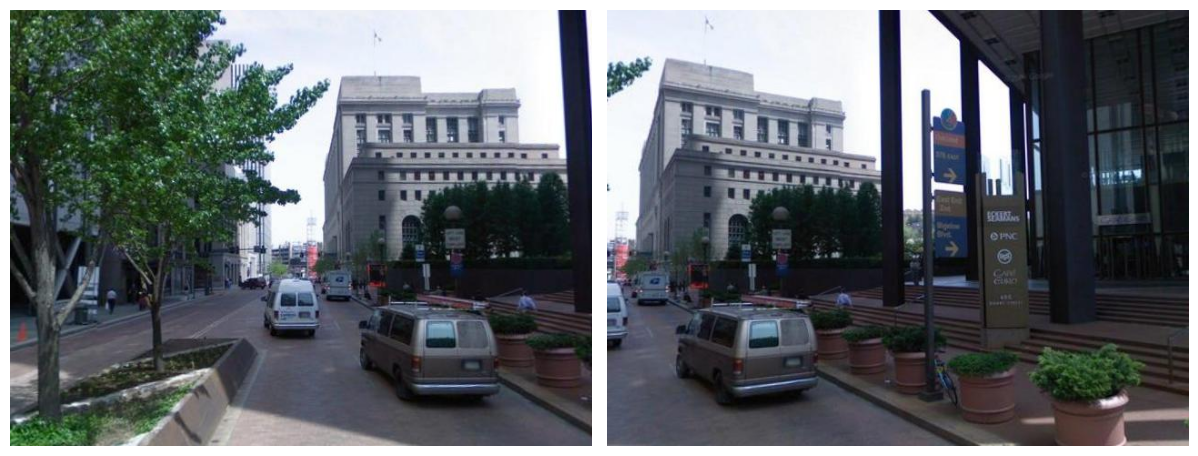
\includegraphics[width=\textwidth]{pics/Chapter3/lowoverlap.png}
%   \caption[Cặp ảnh có độ overlap thấp]{Cặp ảnh không được chấp nhận - có độ trùng lắp thấp}
% \end{figure}

\begin{figure}
  \centering
  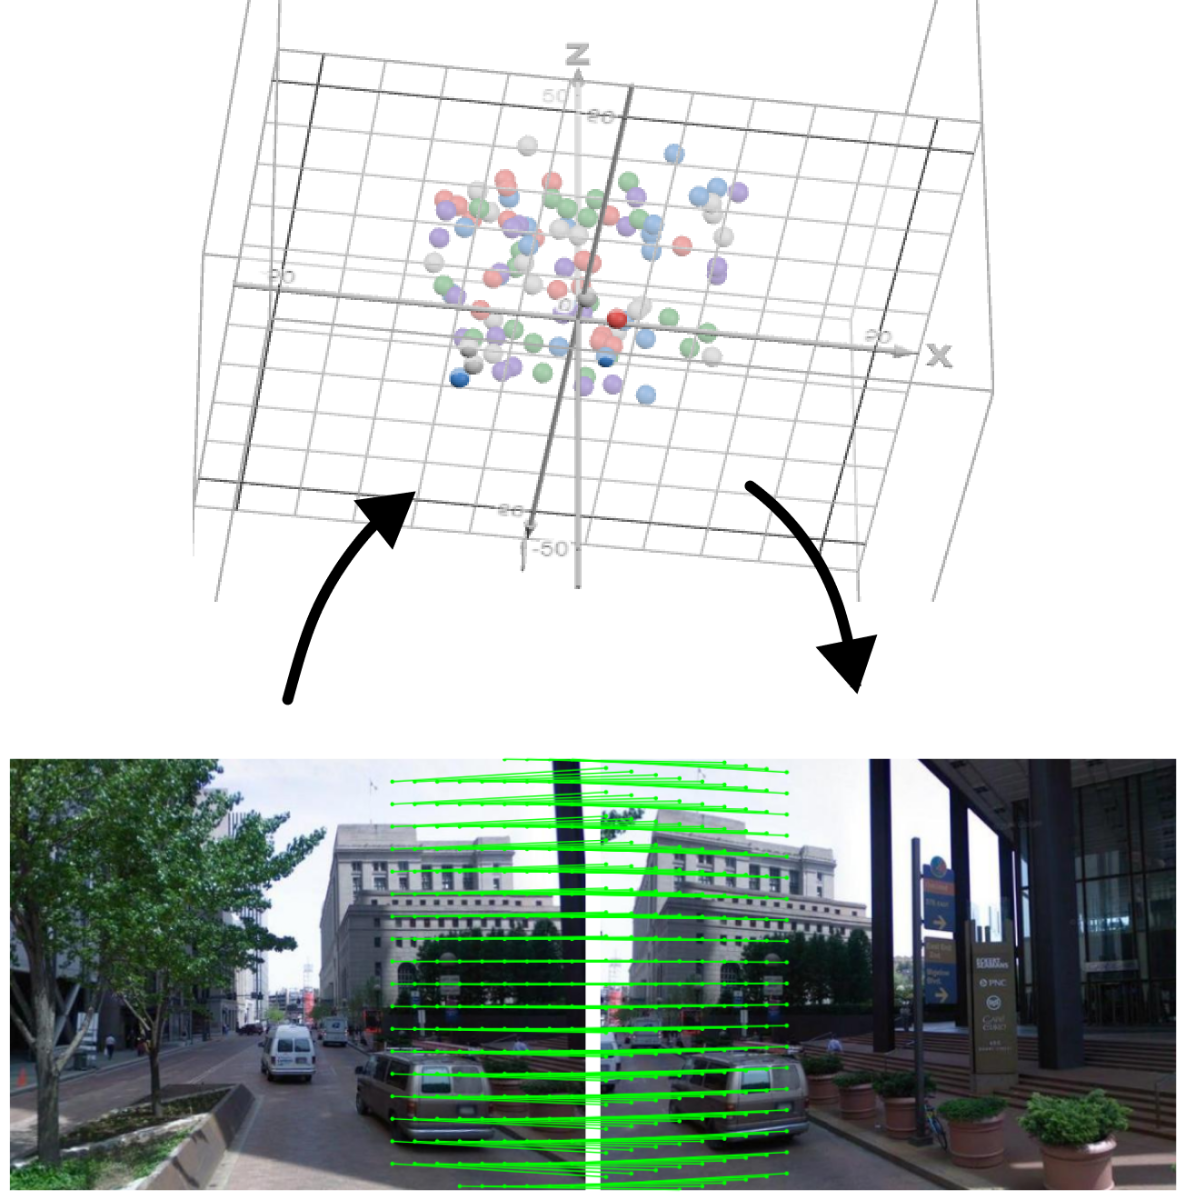
\includegraphics[width=\textwidth]{pics/Proposal/project.drawio.png}
  \caption[Quá trình chiếu giữa 2 ảnh]{Ảnh mô tả quá trình chiếu từ ảnh đầu tiên lên không gian 3D rồi back-project lên không gian khung hình của ảnh thứ 2}
\end{figure}

\subsubsection*{Độ trùng lắp Frustum}

Độ trùng lắp frustum giữa hai ảnh có thể được định nghĩa là tổng tỷ lệ các điểm ảnh thuộc ảnh thứ nhất nằm trong vùng tầm nhìn khi chiếu lên hệ tọa độ camera thứ hai, và ngược lại. Độ trùng lắp này được tính toán bằng cách trước hết chiếu các điểm ảnh từ hình ảnh gốc vào không gian 3D thông qua việc tận dụng độ sâu ước lượng được. Sau đó, các điểm ảnh này được chiếu vào hệ tọa độ của hình ảnh thứ hai bằng cách tận dụng thông tin vị trí và góc quay của chúng.

Đầu tiên, một ma trận các điểm ảnh với kích thước 10x10 được chiếu vào hệ tọa độ thực, sau đó lại được chiếu lại vào hệ tọa độ camera thứ hai. Phép chiếu có thể được công thức hóa như sau:
$$
W = R_1\cdot \left[(K_1^{-1} \cdot P_1)*D_1(P_1)\right] + t_1
$$

$$
P_2 = K_2 \cdot\left[R_2^{T} \cdot (W - t_2)\right]
$$
với $P_i$ là vị trí điểm ảnh trong camera $i$, $K_i$ là ma trận intrinsics, $R_i$ và $t_i$ là độ lệch góc quay và vị trí từ hệ tọa độ camera sang hệ tọa độ thực với $R$ là vector góc quay thu được từ quaternion tương ứng, và $D_i(P)$ là ước lượng độ sâu theo đơn vị khoảng cách của điểm ảnh $P$.

\subsubsection*{Khác biệt hướng nhìn}

Để kiểm soát cách biệt góc quay giữa hai ảnh, chúng tôi đo độ cách biệt về hướng nhìn giữa chúng. Độ lệch góc quay camera $\alpha$ giữa hai camera có thể được định nghĩa như sau:

$$
\alpha = arccos\left(\frac{trace(R_1^T \cdot R_2 - 1)}{2} \right) / \pi * 180
$$

với $\alpha$ mang đơn vị độ và $R_i$ là ma trận 3x3 thể hiện góc quay của ảnh.

\subsubsection*{Hàm Loss}

Hàm loss của chúng tôi được tính toán bằng tổng có trọng số giữa hai hàm loss với một biến số 'Control Rate' - tỷ lệ kiểm soát:
$$
L = \beta * L_{Miner} + (1-\beta)*L_{Control}
$$
với $L_{Control}$ là hàm Multi-Similarity Loss từ bài báo Multi-Similarity Miner và $L_{Miner}$ là hàm Multi-Similarity Loss nhận đầu ra từ chiến lược khai phá frustum mới của chúng tôi và $\beta$ là giá trị tỷ lệ để kiểm soát hai hàm Loss trên.

\subsection{Chiến lược sắp xếp lại ảnh}
Một số nghiên cứu trước đây đã thiết kế tác vụ truy xuất ảnh ở module VPR thành một quá trình gồm 2 bước đi từ kết quả thô đến kết quả chính xác. Việc thực hiện quá trình 2 bước này giúp cho mô hình VPR có thể lọc được tập kết quả thô ban đầu và sau đó tinh chỉnh lại xếp hạng của các kết quả theo một tiêu chí khác. Trong phương pháp đề xuất của chúng tôi, bước truy xuất đầu tiên sẽ được dùng để xác định một tập $k_1$ các ảnh được chụp gần với ảnh truy vấn. Sau đó, bước sắp xếp lại phía sau sẽ sắp xếp lại thứ tự ảnh, sắp xếp theo ưu tiên những ảnh có độ trùng lấp cao với ảnh truy vấn và xác định top $k_2$ ảnh có độ trùng lấp cao nhất.

Với bước truy xuất ban đầu, chúng tôi sử dụng trọng số baseline được cung cấp bởi mô hình MixVPR, do đã được chứng minh là có hiệu quả tốt trong việc xác định ảnh tham khảo có vị trí gần với ảnh truy vấn. Sau đó, ở bước sắp xếp lại thứ tự, chúng tôi sử dụng một trọng số khác của MixVPR đã được huấn luyện lại, tập trung vào việc xác định những ảnh có độ trùng lấp cao với nhau. 

Để có được trọng số mới, chúng tôi huấn luyện mô hình trên tập dữ liệu GSV-Cities \cite{Ali_bey_2022} với mỗi batch sẽ chỉ gồm các ảnh từ 1 khu vực. Mô hình sẽ tập trung vào việc phân biệt những ảnh có độ trùng lấp khung hình cao và thấp theo tiêu chí đã được đặt ra ở \textbf{3.4.1}.

\begin{figure}
  \centering
  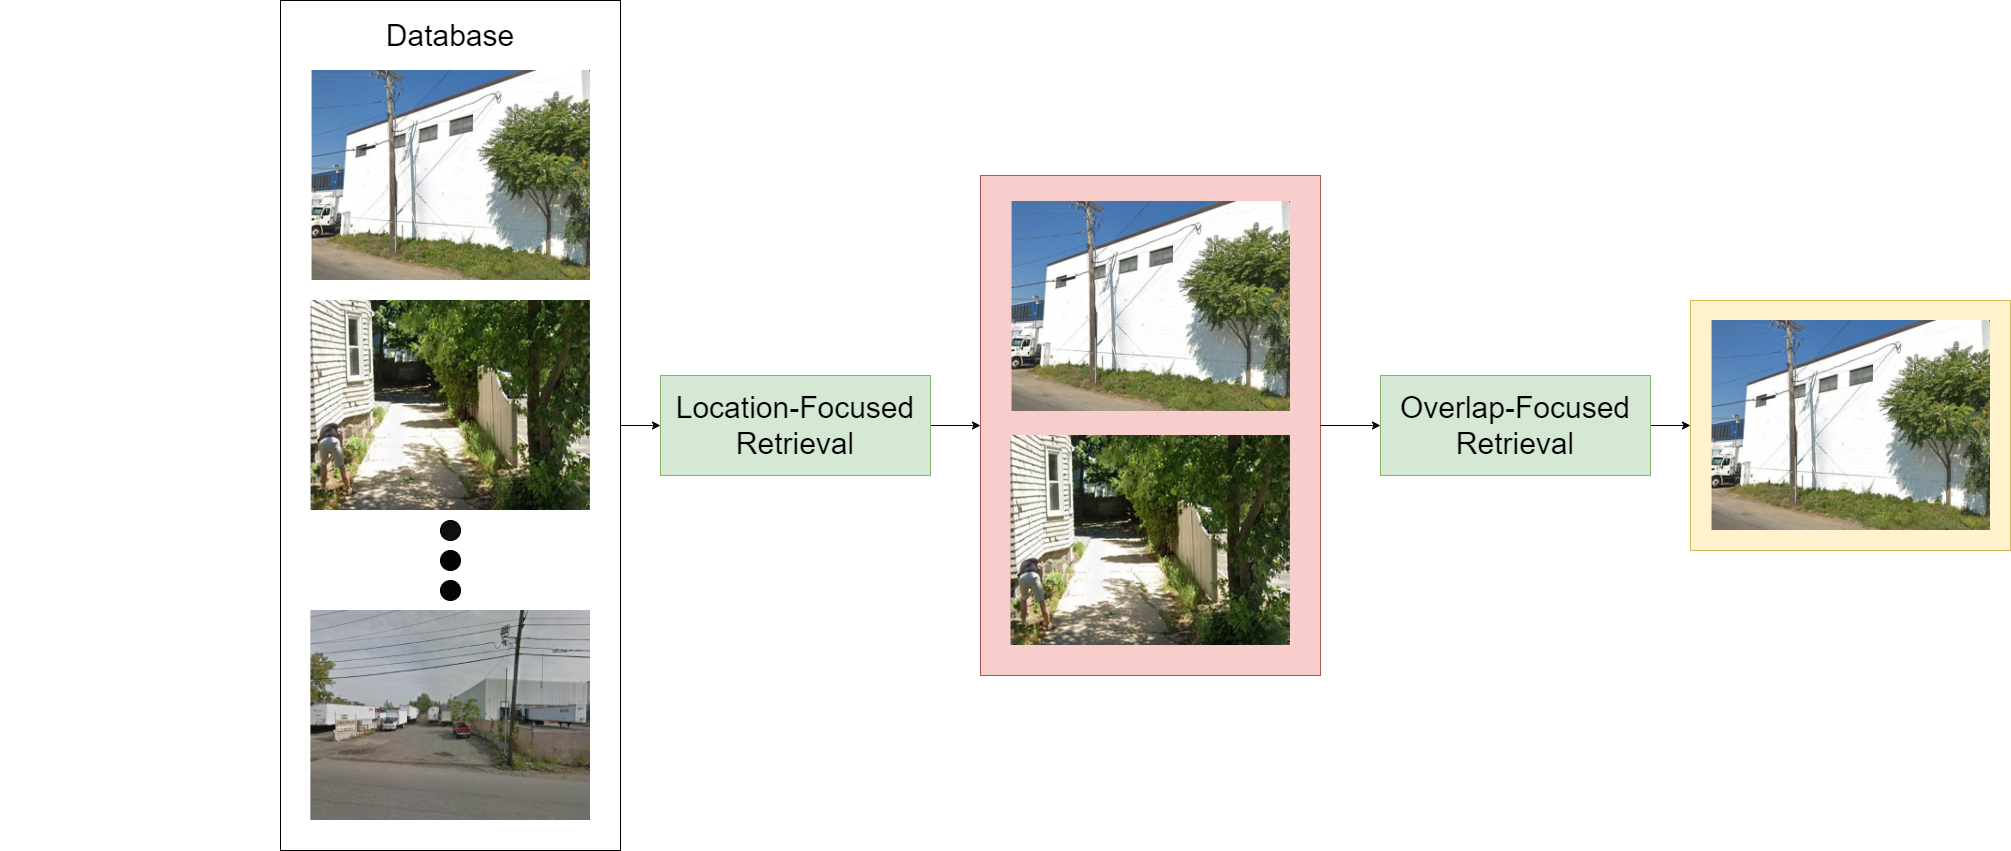
\includegraphics[width=\textwidth]{pics/Proposal/rerank.drawio.png}
  \caption[Quá trình truy xuất 2 bước của VPR]{Quá trình truy xuất gồm 2 bước của mô hình VPR, gồm truy xuất theo địa điểm và truy xuất theo độ trùng lắp}
\end{figure}

\subsection{Trung bình trọng số của các dự đoán}

Ở pipeline cơ bản được đề xuất của nhóm, module VPR sẽ truy xuất được $k$ ảnh tham khảo và từ đó có thể xác định được $k$ dự đoán khác nhau tương ứng với mỗi ảnh. Kết quả cuối cùng sẽ là dự đoán có độ đáng tin cậy $C$ cao nhất. Tuy nhiên, khi chọn theo cơ chế tối đa như thế, thông tin lấy được từ những dự đoán của những ảnh còn lại sẽ bị lãng phí. Vì vậy nên, chúng tôi giới thiệu phương pháp lấy trung bình của từng dự đoán dựa vào với trọng số tương ứng với độ đáng tin $C$.

\begin{figure}[H]
  \centering
  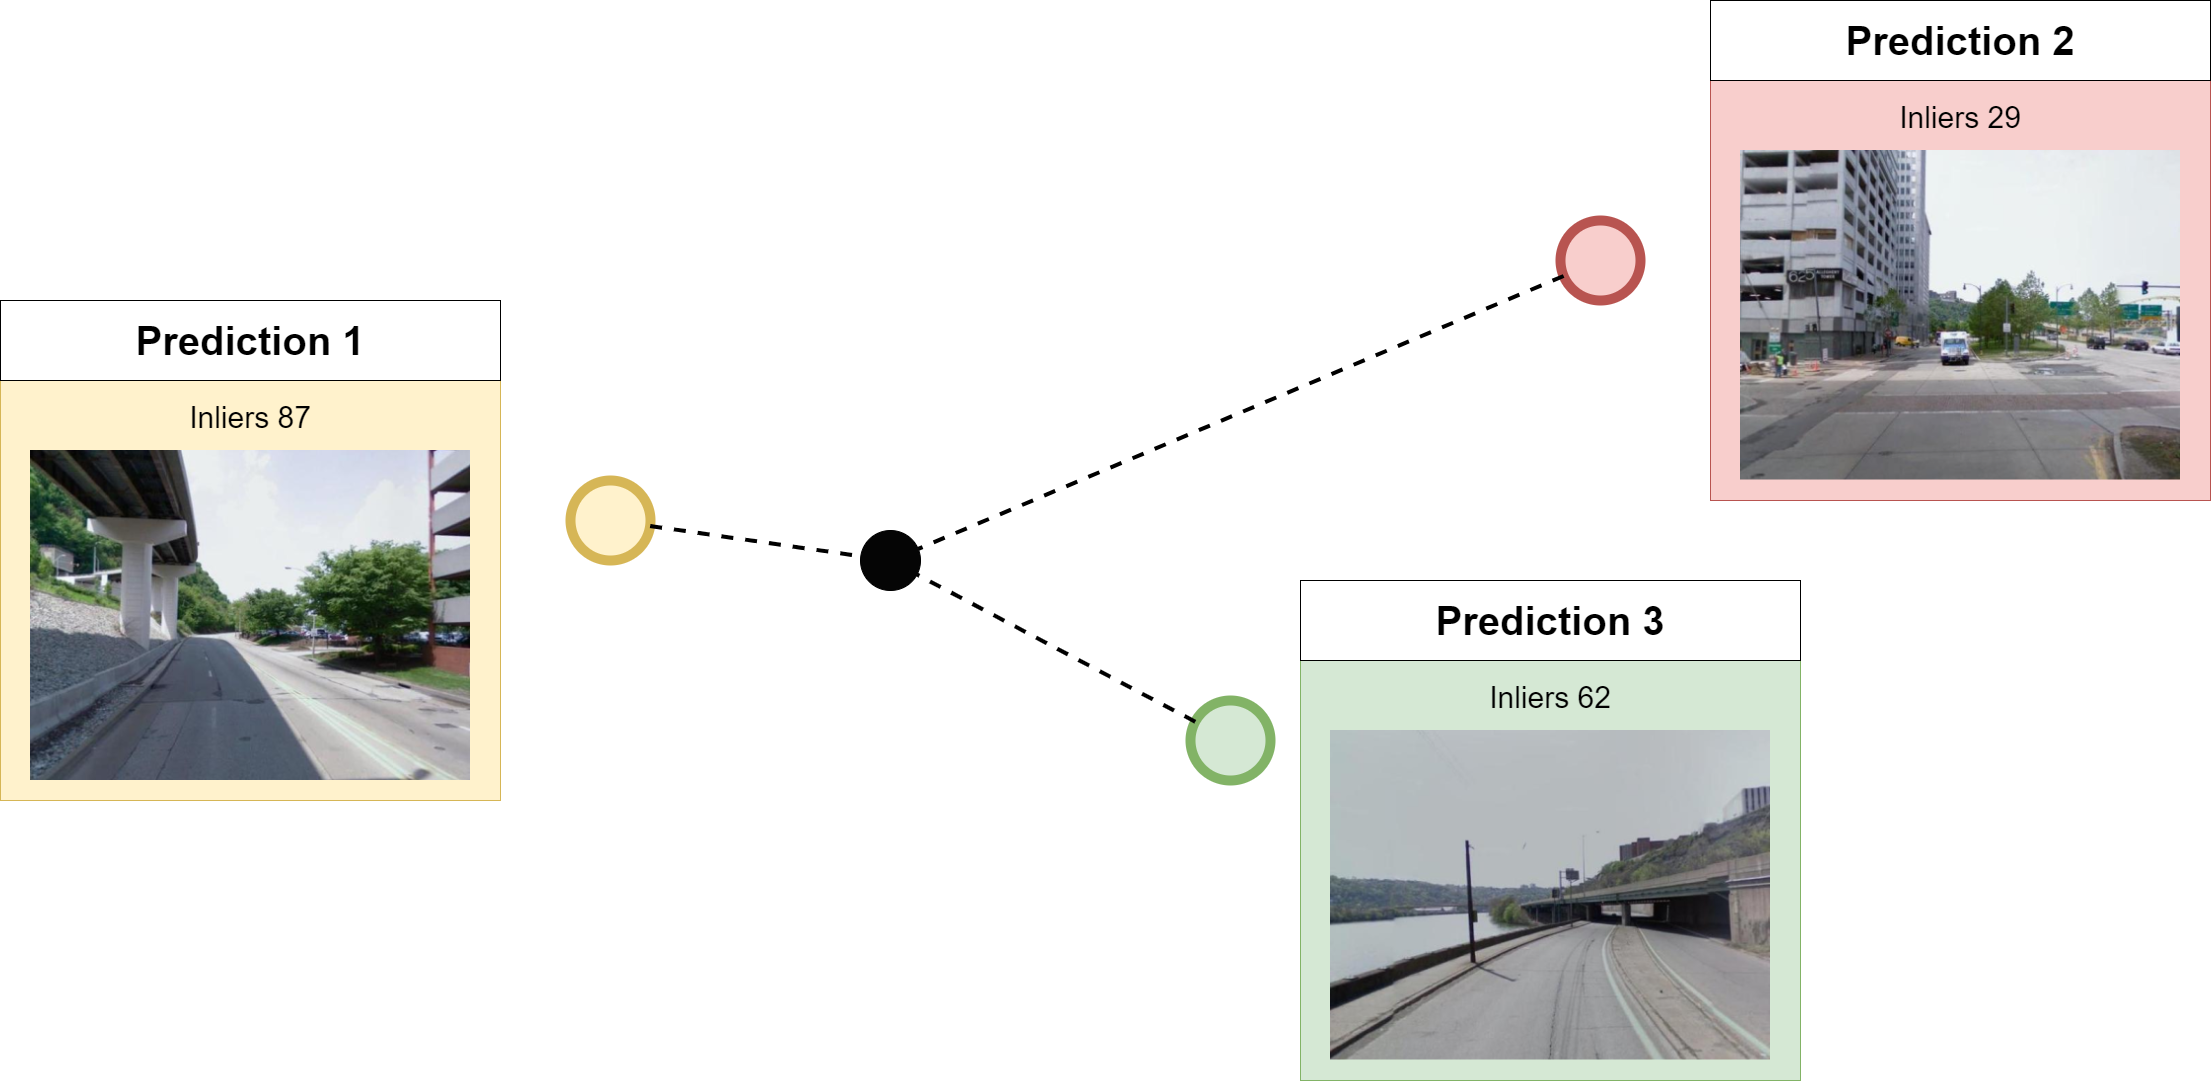
\includegraphics[width=\textwidth]{pics/Proposal/weighted.png}
  \caption[Trung bình trọng số theo inliers của dự đoán]{Mô tả phương pháp lấy trung bình trọng số của các dự đoán theo độ tin cậy của dự đoán}
\end{figure}

\subsection{Giới hạn ngưỡng đáng tin của kết quả}

Độ đáng tin cậy $C$ của dự đoán của cặp ảnh truy vấn và tham khảo được định nghĩa là số cặp điểm tương quan giữa hai hình mà khi áp dụng phép biến đổi tương ứng với độ lệch về tư thế giữa hai ảnh, cho ra độ lệch dưới một ngưỡng nhất định. Càng nhiều điểm thỏa được phép biến đổi thì cơ sở để suy luận ra được độ lệch giữa hai ảnh càng thêm chắc chắn. Vì vậy nên, để đảm bảo được dự đoán của pipeline có thể được tin tưởng, chúng tôi áp dụng một bước lọc lại dự đoán ở cuối pipeline, nhằm lọc ra những kết quả có độ đáng tin cậy thấp, từ đó cải thiện hiệu quả của mô hình.

\begin{figure}[H]
  \centering
  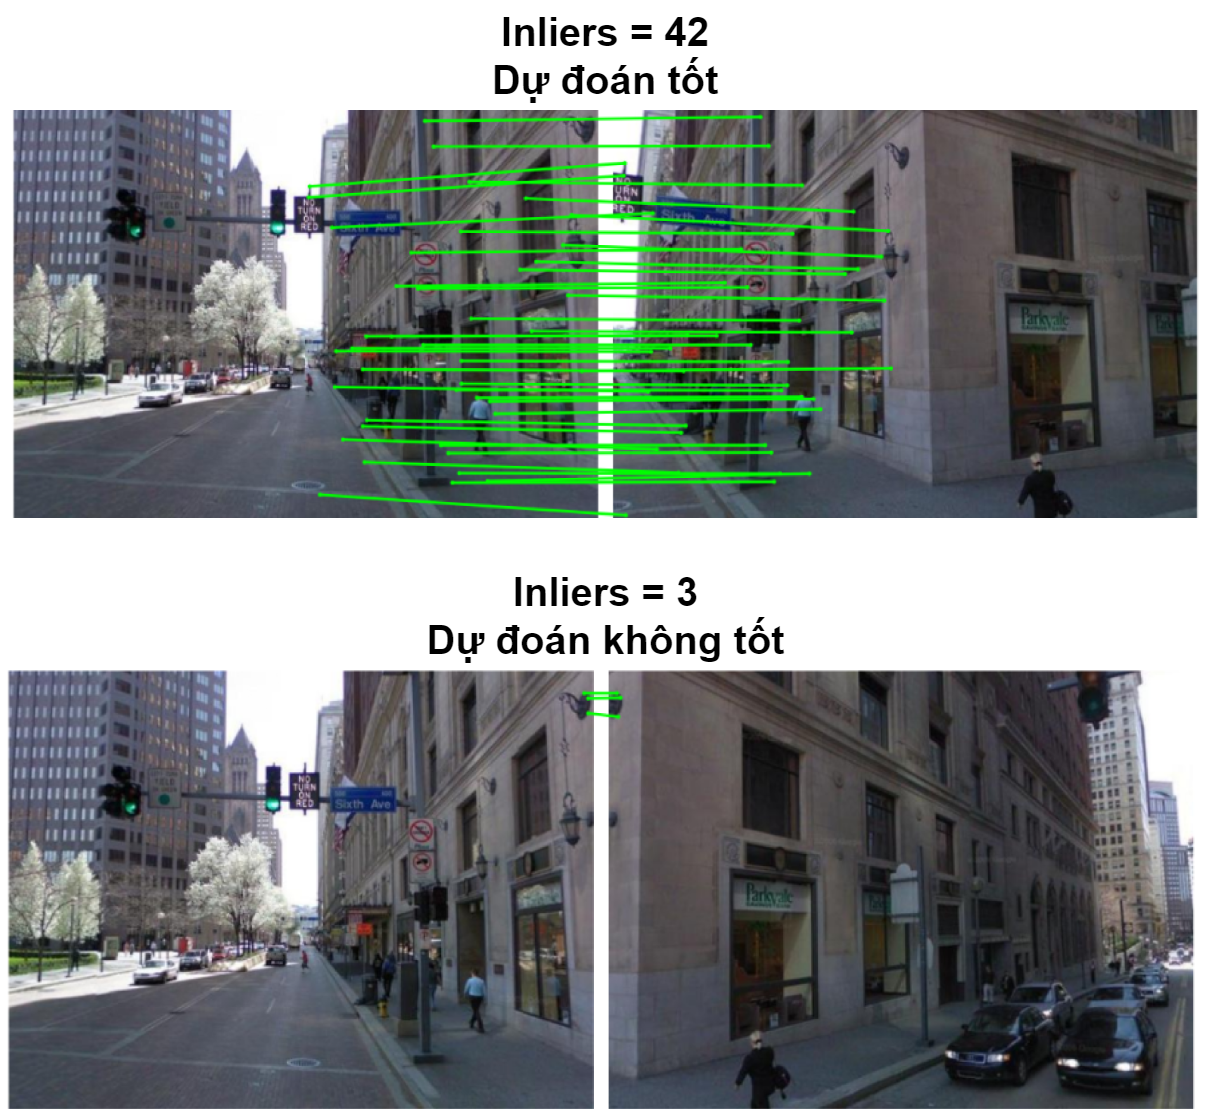
\includegraphics[width=\textwidth]{pics/Proposal/threshold.png}
  \caption[Những dự đoán tốt và không tốt đánh giá theo độ tin cậy]{Mô tả những trường hợp có độ tự tin cao và thấp trong tập dữ liệu Pittsburgh250k \cite{6618963}}
\end{figure}


% \chapter{MÔ HÌNH ĐỀ XUẤT}

\section{Tổng quan về mô hình được đề xuất}
Với đầu vào là một ảnh $I$, mạng MixVPR sẽ tạo ra một tập giá trị mã hóa, đại diện cho ảnh. Giá trị này sẽ được dùng để tìm kiếm ảnh $I'$ có độ tương đồng cao trong tập dữ liệu. Sau khi đã tìm được ảnh tham khảo từ tập dữ liệu, mô hình tương quan 2D-2D của Map-free Relocalization sẽ được sử dụng để xác định độ lệch về vị trí và góc quay giữa ảnh $I$ và $I'$. Cuối cùng, tọa đô tuyệt đối của ảnh $I$ trong không gian sẽ được xác định từ độ lệch và vị trí tuyệt đối của ảnh $I'$.

Như một phương pháp hồi quy vị trí tương đối bình thường, mô hình được đề xuất sẽ bao gồm hai bộ phận chính là bộ phận truy xuất ảnh và bộ phận hồi quy vị trí tương đối dựa trên cặp ảnh. Cụ thể hơn:
\begin{itemize}
    \item Bộ phận truy xuất ảnh sẽ sử dụng mô hình được đề xuất trong bài báo nghiên cứu MixVPR.
    \item Bộ phận hồi quy vị trí tương đối dựa trên cặp ảnh gồm ảnh truy vấn và ảnh tham khảo sẽ sử dụng mô hình tương quan 2D-2D được đề xuất trong bài báo nghiên cứu Map-free Relocalization.
\end{itemize}

\subsection{MixVPR \cite{alibey2023mixvpr}}
\subsubsection*{Ý tưởng đằng sau mô hình}
MixVPR là một phương pháp tổng hợp toàn diện sử dụng Feature Map trích xuất từ một mô hình cơ sở đã được huấn luyện trước đó. MixVPR sẽ lần lượt kết hợp thông tin toàn cục vào mỗi Feature Map thông qua khối Feature Mixer đẳng hướng, được cấu tạo chủ yếu từ những MLP. Khả năng học thông tin toàn cục từ ảnh của MixVPR có thể vượt qua những phương pháp sử dụng cơ chế tập trung như AnyLoc \cite{keetha2023anyloc} trên lĩnh vực ảnh ở khu vực thành thị.

\subsubsection*{Những bước xử lý của mô hình}
\begin{figure}[H]
    \centering
    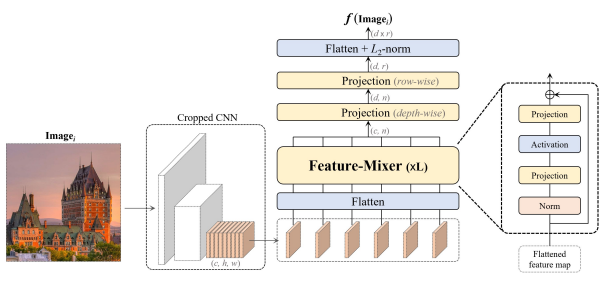
\includegraphics[scale=0.7]{pics/Proposal/mixvpr.png}
    \caption{Tổng quát quá trình xử lý ảnh của MixVPR \cite{alibey2023mixvpr}}
\end{figure}
Với ảnh đầu vào là $I$, mô hình CNN cơ sở sẽ trích xuất ra được tập Feature Map có dạng $F \in R^{c \cdot h \cdot w}$ từ những lớp trung gian.
$$
F = CNN(I)
$$
Ở những phương pháp trước như NetVLAD \cite{arandjelović2016netvlad} và PatchNetVLAD \cite{hausler2021patchnetvlad}, những lớp Feature Map thuộc $F$ sẽ được xem như là một mô tả tương ứng với một miền tiếp nhận trong ảnh ban đầu. Ngược lại, MixVPR xem tensor $F$ như một tập các đặc trưng 2D có kích thước $h \cdot w$.
$$
F = \{X^{i}\}    i = \{1,...c\}
$$
với $X^{i}$ tương ứng với bản đồ kích hoạt thứ $i$ ở F. Ở cách biểu diễn này, mỗi Feature Map không chỉ đại diện cho một miền tiếp nhận trong ảnh mà sẽ chứa một loại thông tin đặc thù cho toàn bộ ảnh. $X^{i}$ sau đó sẽ được định dạng lại thành ma trận một chiều, có được $F \in R^{c \cdot n}$ với $n = h*w$.

Sau đó, dữ liệu sẽ được đưa qua khối Feature Mixer, gồm $L$ những lớp mạng MLP. Những lớp này sẽ nhận vào từng Feature Map $X^{i}$ một chiều và tích hợp thông tin về mối liên kết giữa các giá trị của $X^{i}$ lên chính nó thông qua cách sau:
$$
X^{i} \leftarrow Norm(X^{i})
$$

$$
X^{i} \leftarrow W_2(\sigma(W_1 X^{i}))
$$
với $W_1$ và $W_2$ là trọng số của hai lớp liên kết đầy đủ, cấu tạo nên MLP và $\sigma$ là hàm tạo sự phi tuyến tính cho quá trình xử lý(ReLU). Kỹ thuật nối tắt được sử dụng để nối đầu vào đã qua lớp chuẩn hóa với đầu ra nhằm giúp độ dốc trong quá trình huấn luyện có thể được truyền tải dễ hơn, cải thiện quá trình huấn luyện.

Mục đích của việc sử dụng Feature Mixer là để tận dụng khả năng tổng hợp thông tin từ dữ liệu của các lớp kết nối đầy đủ, thay vì học trên những đặc trưng cục bộ trên ảnh và sử dụng cơ chế tập trung. Ngoài ra, Feature Mixer cũng sẽ trả về kết quả có định dạng như cũ, thay vì có đầu ra giảm dần như những phương pháp tổng hợp dạng phân cấp(kim tự tháp) như trước đây, để mỗi nơ-ron đều có thể biết được thông tin của toàn bộ ảnh. Những lớp MLP trong khối Feature Mixer sẽ giúp tích hợp thông tin trên toàn bộ ảnh qua mỗi lần xử lý.

Mỗi khối Feature Mixer sau khi xử lý xong từng Feature Map trong tập $F \in R^{c \cdot n}$, sẽ ghép kết quả lại, tạo thành $Z \in R^{c \cdot n}$ với cùng kích thước trước khi được đưa vào khối Feature Mixer kế tiếp. Quá trình này có thể được miêu tả bằng công thức sau:
$$
Z = FM_L(FM_{L-1}(\dots FM_1(F)))
$$
Số chiều của $Z$ thường sẽ rất cao do có định dạng được giữ nguyên so với $F$. Để giúp giảm bớt số chiều của $Z$ lại sau khi qua khối Feature Mixer, hai lớp kết nối đầy đủ sẽ được sử dụng để tổng hợp giữa các kênh với nhau và sau đó là giữa các giá trị trong từng kênh. Tác vụ này thực hiện việc tổng hợp có chọn lọc nhằm điều khiển được kích thước của giá trị đầu ra.

Đầu tiên, dữ liệu sẽ được tổng hợp số kênh để biến định dạng của $Z$ từ $R^{c \cdot n}$ thành $R^{d \cdot n}$.
$$
Z' = W_d(Transpose(Z))
$$
với $W_d$ là trọng số của lớp kết nối đầy đủ đầu tiên.

Sau đó, giá trị trên từng kênh sẽ được tổng hợp lại, từ định dạng $R^{d \cdot n}$ thành $R^{d \cdot r}$.
$$
O = W_r(Transpose(Z'))
$$
với $W_r$ là trọng số của lớp kết nối đầy đủ thứ hai.

Kết quả $O$ cuối cùng, có định dạng là $R^{d \cdot r}$, sẽ được ép thành một chiều và chuẩn hóa theo L2 như những phương pháp VPR khác \cite{arandjelović2016netvlad,berton2022rethinking}. Cuối cùng, từ ảnh đầu vào $I$, mô hình sẽ trả về một đoạn mã hóa biểu diễn cho nội dung của ảnh. Đoạn mã hóa này sau đó có thể được dùng để so sánh với giá trị mã hóa của những hình khác nhằm tìm ảnh có độ tương đồng cao nhất với $I$.

\subsubsection*{Chi tiết hiện thực phương pháp}
\textbf{Cấu trúc:} Phương pháp tổng hợp sử dụng mô hình MixVPR sẽ được hiện thực trên framework PyTorch. Mô hình CNN cơ sở của MixVPR sẽ được cắt ở lớp áp cuối của mô hình ResNet. Dữ liệu đầu vào cho MixVPR sẽ là một tập các Feature Map có kích thước 20x20. Thao tác tổng hợp trong khối Feature Mixer sẽ sử dụng lớp Linear được cung cấp bởi PyTorch, theo sau đó là một lớp ReLU để tạo tính phi tuyến tính. Với lớp chuẩn hóa, LayerNorm của PyTorch sẽ được sử dụng. Cuối cùng, đầu ra cuối cùng của khối Feature Mixer sẽ được tổng hợp xuống một chiều không gian biểu diễn nhỏ hơn sử dụng hai lớp kết nối đầy đủ giữa các kênh với nhau và giữa các giá trị trong mỗi kênh, chứng minh là MixVPR là một cấu trúc chỉ sử dụng MLP. Số khối Feature Mixer được sử dụng sẽ luôn được giữ là $L=4$ trừ khi được quy định khác.

\textbf{Huấn luyện:} Mô hình MixVPR được đánh giá trong bài nghiên cứu sẽ sử dụng mô hình ResNet \cite{he2016deep} đã được huấn luyện trên tập ImageNet \cite{krizhevsky2012imagenet} làm cơ sở. Sau đó, mô hình sẽ được huấn luyện trên tập dữ liệu GSV-Cities \cite{Ali_bey_2022}. Đối hàm mất mát, hàm Multi-Similarity Loss \cite{wang2019multi} do hàm đã được chứng mình là hỗ trợ cho ra kết quả tốt với tác vụ VPR \cite{Ali_bey_2022}. Kích thước của một batch sẽ có $P$ = 120 địa điểm, mỗi địa điểm được miêu tả bởi 4 ảnh, tạo thành một batch có kích thước 480 ảnh. Phương tối ưu giảm độ dốc ngẫu nhiên - SGD sẽ được sử dụng với quán tính - momentum là 0.9 với giá trị suy giảm trọng số - weight decay là 0.001. Tốc độ học - learning rate sẽ được khởi tạo với giá trị 0.05 và sẽ được chia 3 sau mỗi 5 chu kỳ - epoch. Cuối cùng, mô hình sẽ được huấn luyện tối đa 30 chu kỳ - epoch với đầu vào là ảnh đã được chỉnh xuống kích thước 320x320.

\textbf{Đánh giá:} Để đánh giá, 5 tiêu chuẩn sẽ được sử dụng. Pitts250k-test \cite{6618963}, bao gồm 8k ảnh truy vấn và 83k ảnh tham khảo, được thu thập từ Google Street View và Pitts30k-test \cite{6618963} là một tập con của Pitts250k bao gồm 8k ảnh truy vấn và 8k ảnh tham khảo. Cả 2 tập dữ liệu Pittsburgh đều có những góc nhìn có độ lệch đáng kể. Tập dữ liệu SPED \cite{zaffar2021vpr} gồm 607 ảnh truy vấn và 607 ảnh tham khảo từ camera giám sát chứa những thay đổi lớn về độ sáng và về cảnh vật các mùa. MSLS \cite{warburg2020mapillary} được thu thập từ camera hành trình của xe hơi và cho rất nhiều góc nhìn đa dạng và sự thay đổi về độ sáng. Cuối cùng, Nordland \cite{zaffar2021vpr} là một tập dữ liệu chứa nhiều thử thách khi sử dụng ảnh thu thập được ở cả 4 mùa với camera được gắn trên tàu. Đơn vị đánh giá được sử dụng sẽ là recall@k, thể hiện tỷ lệ của truy xuất thành công trên tổng số lượng truy xuất. Một truy xuất hình sẽ được xem là thành công khi ảnh được truy xuất nằm trong vòng 25m xung quanh ảnh truy vấn.

\subsubsection*{Hiệu quả của phương pháp}
Khi so sánh trên những tập dữ liệu phản ánh môi trường thành thị, phương pháp sử dụng mô hình MixVPR đạt được kết quả vượt trội so với những mô hình SOTA đã được đề xuất trước nó, như CosPlace \cite{berton2022rethinking} và NetVLAD \cite{arandjelović2016netvlad}. Những tập dữ liệu được sử dụng đã bao quát hết những trường hợp có thể tác động xấu đến mô hình như góc nhìn đa dạng; thời tiết, mùa thay đổi; chênh lệch về độ sáng.

MixVPR cũng có khả năng giải quyết được những trường hợp mà những phương pháp trước gặp khó khăn như:
\begin{itemize}
    \item Kiến trúc lặp lại nhiều
    \item Góc nhìn thay đổi rõ rệt
    \item Đường chân trời
    \item Độ sáng chênh lệch lớn
    \item Gặp nhiều vật thể cản trở tầm nhìn
\end{itemize}
Tuy nhiên, mô hình vẫn sẽ gặp thất bại khi độ chênh lệch góc nhìn là quá lớn hoặc có quá nhiều vật cản.

\begin{figure}[H]
    \centering
    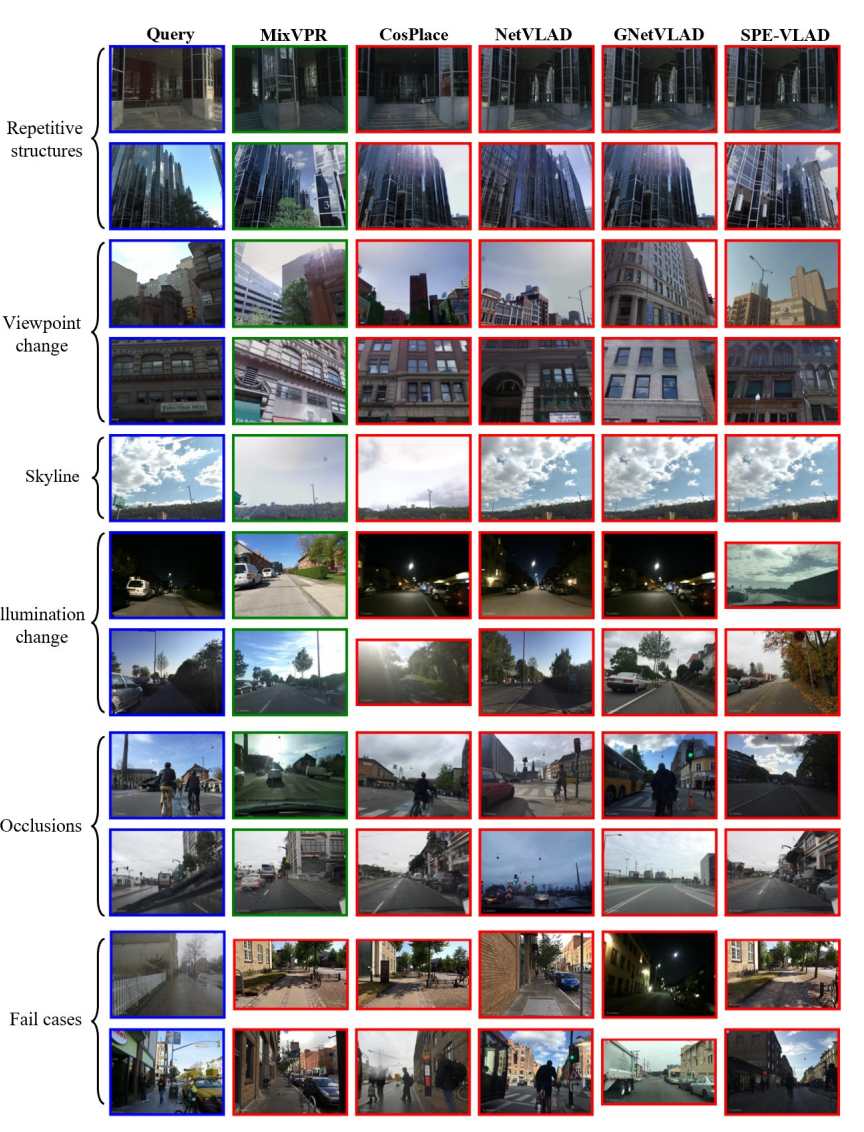
\includegraphics[scale=0.5]{pics/Proposal/fail.png}
    \caption{Kết quả của những trường hợp khó khi chạy trên MixVPR và các phương pháp khác \cite{alibey2023mixvpr}}
\end{figure}

Với sự ra đời của AnyLoc \cite{keetha2023anyloc}, bài toán VPR trong những môi trường đa dạng hơn như trong nhà, trong hang động, trên bầu trời, hoặc trên mặt biển đã có một SOTA mới. Điều này là nhờ việc AnyLoc sử dụng mạng cơ sở DINO, một mạng Vision Transformer được huấn luyện bằng cơ chế tự giám sát để sinh ra những đặc trưng có giá trị với mọi tác vụ. Tuy nhiên, khi xét đến môi trường thành thị thì MixVPR vẫn có cho ra kết quả chính xác hơn AnyLoc. Số liệu cụ thể sẽ được trình bày bên dưới.

\begin{figure}[H]
    \centering
    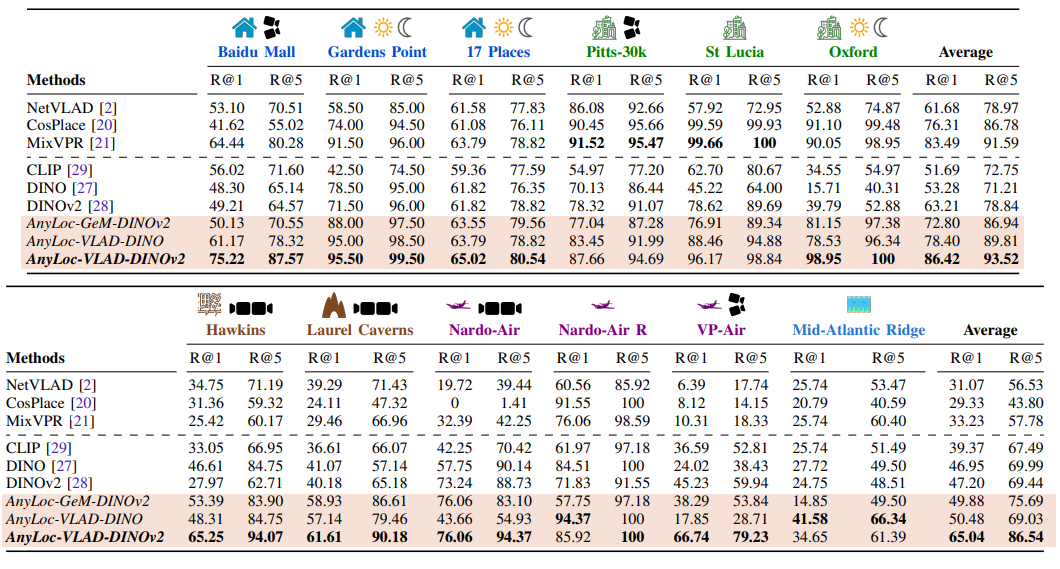
\includegraphics[scale=0.5]{pics/Proposal/anyloc.png}
    \caption{Kết quả của AnyLoc so sánh với những mô hình khác \cite{keetha2023anyloc}}
\end{figure}



\subsection{Mô hình tương quan 2D-2D của Map-free Relocalization \cite{arnold2022mapfree}}
\subsubsection*{Ý tưởng đằng sau mô hình}
Mô hình tương quan 2D-2D được đề xuất trong Map-free Relocalization thuộc nhóm những phương pháp sử dụng tìm kiếm cặp đặc trưng tương quan trong ảnh và xác định quy mô qua ước tính độ sâu. Phương pháp này sẽ giải quyết được điểm yếu của những phương pháp RPR là không nắm bắt được thông tin về hình học trong ảnh bằng cách sử dụng cách biểu diễn trung gian là ma trận thiết yếu. Dù kết quả của mô hình trong những môi trường có tập dữ liệu ảnh biểu diễn phân bố dày đặc là không quá vượt trội. Tuy nhiên, khi phân bố ảnh trong tập dữ liệu trở nên thưa hơn trong không gian đang xét thì phương pháp 2D-2D lại có kết quả vượt qua phương pháp 2D-3D và 3D-3D. 
\subsubsection*{Những bước xử lý của mô hình}

Với đầu vào là cặp ảnh $(I_0,I_1)$, những cặp đặc trưng tương quan giữa hai ảnh sẽ được xác định thành 2 tập là $(kpts_0, kpts_1)$ tương ứng với mỗi hình. Sau đó, ma trận thiết yếu giữa 2 ảnh sẽ được ước tính dựa vào giải thuật 5 điểm \cite{nister2004efficient} cùng với MAGSAC++ \cite{barath2020magsac++} dựa trên 2 tập điểm tương quan đã được xác định. Ma trận thiết yếu sau đó sẽ được phân giải thành ma trận thể hiện góc quay chênh lệch, $R \in SO(3)$ và vector đơn vị độ lệch về vị trí giữa hai ảnh, $\hat{t} \in R^{3}, \lvert \hat{t} \rvert = 1$.

Các cặp điểm tương quan giữa hai ảnh thỏa ma trận thiết yếu sẽ được chiếu lên không gian 3D qua độ sâu của ảnh. Với mỗi cặp điểm $(p_0,p_1)$, một tỷ lệ $s$ có thể được xác định bằng công thức:
$$
\begin{aligned}
    s=\underset{s^*}{\arg \min }\left\|R p_A+s^* \cdot \hat{t}-p_B\right\|_2 .
\end{aligned}
$$

\begin{figure}[H]
    \centering
    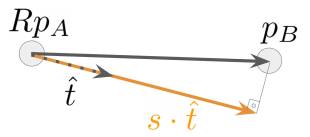
\includegraphics[scale=0.8]{pics/Proposal/reprojection.png}
    \caption[Minh họa cho việc xác định tỷ lệ $s$ bằng độ sâu ảnh]{Hình minh họa cho việc chiếu điểm $p_0$ qua vector góc quay $R$ và vector độ lệch đơn vị $\hat{t}$ cùng với tỷ lệ $s$ để tối thiểu khoảng cách \cite{arnold2022mapfree}}
\end{figure}


Mỗi cặp tương quan sẽ trả về một tỷ lệ $s$ cho vector đơn vị độ lệch. Vòng lặp RANSAC sẽ được sử dụng để loại bỏ những trường hợp ngoại lệ sinh ra từ việc ước lượng độ sâu sai lệch. Sau đó, giá trị $s$ có số cặp điểm hợp lệ lớn nhất sẽ được chọn để kiếm được vector độ lệch. Một cặp điểm sẽ được coi là hợp lệ nếu khoảng cách giữa hai điểm sau phép chiếu nhỏ hơn một giá trị nhất định. Trong bài nghiên cứu, giá trị 10cm được chọn.

\subsubsection*{Chi tiết hiện thực phương pháp}

\textbf{Cấu trúc:} Tác vụ tìm kiếm tương quan giữa hai ảnh sẽ có thể lựa chọn giữa phương pháp truyền thống như SIFT, hoặc những phương pháp theo hướng tiếp cận học sâu gần đây hơn như SuperPoint+SuperGlue \cite{sarlin2020superglue} và LoFTR \cite{sun2021loftr}. Tác vụ tính độ sâu đơn ảnh sẽ được phân thành hai trường hợp là bên trong nhà và ngoài trời. Với những tập dữ liệu trong nhà, mô hình DPT \cite{ranftl2021vision} được huấn luyện trên tập dữ liệu NYUv2 \cite{silberman2012indoor} PlaneRCNN \cite{liu2019planercnn} được huấn luyện trên tập dữ liệu ScanNet \cite{dai2017scannet}. Với trường hợp ngoài trời, mô hình DPT \cite{ranftl2021vision} được huấn luyện trên tập KITTI sẽ được sử dụng \cite{geiger2012we}.

\textbf{Đánh giá:} Để đánh giá hiệu quả của mô hình trong tác vụ định vị trực quan, một số tiêu chí cơ bản đã được đưa ra như độ lệch về góc quay, độ lệch về vị trí của máy ảnh, cũng như một sai số mới được đưa ra trong bài nghiên cứu, sai số phản chiếu của điểm 3D ảo - VCRE, được lấy cảm hứng từ sai số phản chiếu của những điểm tương ứng - DCRE \cite{wald2020beyond}. Cụ thể, với giá trị dự đoán $(R,t)$ và giá trị thực $(R_{gt},t_{gt})$, các sai số sẽ được xác định như sau:
\begin{itemize}
    \item Sai số về góc quay, $\measuredangle(R,R_{gt})$, sẽ được tính là độ chênh lệch giữa góc quay được dự đoán và góc quay thực tế.
    \item Sai số về độ lệch máy quay sẽ được tính là khoảng cách Euclidian giữa cặp vị trí $(c,c_{gt})$ được tính theo công thức $c=-R \intercal t$.
    \item Sai số phản chiếu của điểm 3D ảo sẽ được dùng để đánh giá độ lệch của những vật thể trong không gian thực tế ảo. Giá trị thực $(R_{gt},t_{gt})$ và giá trị dự đoán $(R,t)$ sẽ được dùng để chiếu những điểm 3D ảo, lên hệ tọa độ của camera truy vấn. Giá trị VCRE sẽ được xác định theo công thức
    $$
    \operatorname{VCRE}=\frac{1}{|\mathcal{V}|} \sum_{\mathbf{v} \in \mathcal{V}}\left\|\pi(\mathbf{v})-\pi\left(T T_{\mathrm{gt}}^{-1} \mathbf{v}\right)\right\|_2 \quad \text { với } T=[R \mid t]
    $$

    với $\pi$ là phép chiếu từ không gian camera lên ảnh, $\mathcal{V}$ là một tập các điểm 3D, đại diện cho những vật thể ảo. $\mathcal{V}$ là một lưới điểm 3D, (chiều cao là 4, chiều rộng là 7 và chiều sâu là 7), cách nhau 30cm và có độ dịch là 1.8m dọc theo trục của máy ảnh. Giá trị sai số của phép phản chiếu sẽ được so sánh với đường chéo của ảnh.
    \item Độ tin cậy của dự đoán cũng là một tiêu chí được đánh giá. Giá trị này cho phép mô hình có thể phát hiện và loại bỏ những dự đoán không đáng tin cậy. Giá trị này sẽ được xác định bằng số lượng cặp điểm tương quan thỏa ma trận thiết yếu được chọn trên tổng số cặp điểm tương quan xác định bởi mô hình ghép đặc trưng. Với một ngưỡng tin cậy nhất định, tỷ lệ dự đoán đáng tin cậy - ratio of confident estimate, sẽ được xác định là tỷ lệ của những ảnh truy vấn có độ tin cậy vượt qua ngưỡng.
    \item Độ chính xác của mô hình sẽ là tỷ lệ của những ảnh đáng tin cậy có sai lệch giữa giá trị dự đoán và giá trị thực dưới một ngưỡng nhất định (độ lệch vị trí và góc quay) hoặc có sai số phản chiếu chấp nhận được trên tổng số ảnh.
\end{itemize}

Tập dữ liệu 7Scenes \cite{6619221} sẽ được sử dụng để xác định hiệu quả của mô hình tiêu chuẩn của Mapfree sẽ có hiệu quả như thế nào so với những phương pháp SOTA tại thời điểm đó, với số lượng ảnh tham khảo là rất nhiều. Ảnh hưởng của việc giảm số lượng ảnh tham khảo lên khả năng hoạt động của các mô hình cũng sẽ được ghi nhận lại. Tập dữ liệu Niantic được đề xuất trong cùng bài nghiên cứu cũng sẽ được sử dụng để đánh giá, nhằm xác định hiệu quả của các mô hình trong trường hợp chỉ có một ảnh tham khảo.

\subsubsection*{Hiệu quả của phương pháp}

\textbf{Tập dữ liệu 7Scenes \cite{6619221}}

\begin{figure}[H]
    \centering
    \includegraphics[scale=0.8]{pics/Proposal/all_7scene.png}
    \caption[Bảng so sánh hiệu quả của các mô hình trên tập 7Scenes]{Hiệu quả của những mô hình khi có đầy đủ ảnh tham khảo trên tập 7Scenes. Những phương pháp \textcolor{green}{xanh lá} sẽ phụ thuộc vào tập dữ liệu, phương pháp \textcolor{yellow}{vàng} được huấn luyện trên SUNCG \cite{song2017semantic} và \textcolor{blue}{xanh dương} trên tập ScanNet \cite{dai2017scannet}}
\end{figure}

Khi xét trên tập dữ liệu 7Scenes với tất cả các ảnh tham khảo, những phương pháp sử dụng biểu diễn 3D như DSAC* \cite{brachmann2021visual}, hLoc \cite{sarlin2019coarse}, ActiveSearch \cite{sattler2016efficient} có kết quả tốt nhất, tuy nhiên lại phụ thuộc vào quá trình tái tạo lại cấu trúc. Những phương pháp sử dụng phép đạc tam giác, sử dụng 5 ảnh tham khảo có kết quả cạnh tranh so với những phương pháp sử dụng biểu diễn 3D, được ký hiệu bằng $\triangle$. 

Để thực hiện bài toán định vị không cần biểu diễn, chỉ một ảnh tham khảo sẽ được sử dụng cho một truy vấn cho những phương pháp trong tập \textit{hồi quy vị trí tương đối} và \textit{ghép cặp đặc trưng + độ sâu ảnh}. Cả hai lớp phương pháp đều có kết quả bị xuống cấp, với phương pháp ghép cặp + độ sâu tốt hơn những phương pháp hồi quy tương đối. Tuy nhiên, các phương pháp thuộc các lớp vẫn có kết quả cạnh tranh, có thể được phần nào giải thích bởi việc truy xuất ảnh tốt và sự phân bố dày đặc của tập dữ liệu.

\begin{figure}[H]
    \centering
    \includegraphics[scale=0.8]{pics/Proposal/partial_7scene.png}
    \caption[Hiệu quả của các mô hình khi giới hạn ảnh tham khảo]{Hiệu quả của những mô hình khi tập 7Scenes chỉ có 10/1 ảnh tham khảo, đánh giá về độ chính xác và về số ảnh có sai số phản chiếu dưới ngưỡng.}
\end{figure}

Để có thể phản ánh một môi trường thực, nơi mà ảnh tham khảo truy xuất được cách xa đáng kể so với ảnh truy vấn, $K$ ảnh tham khảo mang nhiều thông tin nhất sẽ được chọn làm đại diện qua giải thuật gom cụm K-means.

Với việc so sánh độ chính xác ở hai kịch bản, ngưỡng chấp nhận về độ chính xác sẽ là $VCRE<10\%$ của đường chéo ảnh(80px). Khi ngưỡng tin cậy được hạ thấp, điều này làm cho tỷ lệ dự đoán đáng tin cậy tăng lên. Điều này làm độ chính xác giảm dần, do chứa những trường hợp có độ tin cậy không đủ cao. Trong trường hợp này, những mô hình 2D-2D, đặc biệt là mô hình sử dụng SuperGlue, có kết quả tốt hơn so với những mô hình còn lại, đặc biệt trong khoảng $0.5~1.0$. Ngoài ra, mô hình 2D-2D có thể tính ra vị trí và góc quay của hơn 50\% ảnh với VCRE < 40px.

Mô hình DSAC* vẫn có kết quả tốt nhất trong các mô hình. Tuy nhiên, phương pháp này lại phụ thuộc vào tập dữ liệu. Trong khi đó, những mô hình khác được huấn luyện trên tập ScanNet vẫn có kết quả tốt trên tập 7Scenes. Phương pháp sử dụng phép đạc tam giác cũng có kết quả cạnh tranh, tuy nhiên lại không thể hoạt động chỉ với một ảnh tham khảo. Những phương pháp ghép cặp + độ sâu có khả năng khái quát hóa tốt hơn những phương pháp RPR, như có thể thấy ở hiệu quả thấp hơn của những phương pháp hồi quy tương đối.

\textbf{Tập dữ liệu Niantic \cite{arnold2022mapfree}}

\begin{figure}[H]
    \centering
    \includegraphics[scale=0.4]{pics/Proposal/all_niantic.png}
    \caption{Hiệu quả của các mô hình trên tập dữ liệu Niantic, xác định theo độ chính xác và số ảnh có sai số phản chiếu dưới ngưỡng}
\end{figure}

Qua kết quả thu được, tập dữ liệu Niantic có độ khó cao hơn đáng kể so với tập dữ liệu 7Scenes với mọi phương pháp. Điều này có thể thấy được rõ ràng từ kết quả của các mô hình. Trong tập dữ liệu Mapfree, những phương pháp 2D-2D tiếp tục có kết quả tốt. Tuy nhiên, ở những ngưỡng VCRE rộng hơn, những phương pháp RPR lại có kết quả tốt hơn. Điều này có thể giải thích được qua việc khi số cặp đặc trưng tương quan là không đủ chất lượng, độ lệch đơn vị vị trí được sinh ra có thể có sai số rất lớn so với thực tế. Vậy nên, những phương pháp RPR sẽ cho ra kết quả tốt khi ngưỡng chính xác rộng, nhưng lại có kết quả không tốt khi cần độ chính xác cao. Ngoài ra, những phương pháp RPR cũng không thể cung cấp độ tin cậy cho dự đoán của mô hình, hạn chế việc loại bỏ những dự đoán có khả năng sai cao.

\section{Mô hình đề xuất}
Sau những nghiên cứu và tìm hiểu, nhóm quyết định đề xuất một mô hình kết hợp giữa MixVPR \cite{alibey2023mixvpr}và Map-free Relocalization \cite{arnold2022mapfree}. Gọi $I$ là ảnh mà người dùng chụp từ máy ảnh và sẽ được dùng làm ảnh truy vấn cho mô hình đề xuất của nhóm. Trước hết, mô hình sẽ nhận $I$ và truyền làm đầu vào cho MixVPR. Từ ảnh đầu vào $I$, sau khi qua các giai đoạn xử lý, MixVPR sẽ trả về một đoạn mã hóa biểu diễn cho nội dung của ảnh. Với đoạn mã hóa này, mô hình tiến hành so sánh với giá trị mã hóa của các ảnh trong cơ sở dữ liệu và tìm ra ảnh có sự tương đồng cao nhất với ảnh nhận vào $I$ gọi là $I_0$.

Bước tiếp theo, mô hình tiếp tục truyền cả ảnh nhận vào $I$ và ảnh được truy xuất $I_0$ cho mô hình tương quan 2D - 2D của Map-free Relocalization \cite{arnold2022mapfree}. Với đầu vào là cặp ảnh $(I, I_0)$, những cặp đặc trưng tương quan giữa hai ảnh sẽ được xác định tương ứng với mỗi hình. Sau đó, ma trận thiết yếu $E$ giữa 2 ảnh sẽ được ước tính dựa vào giải thuật 5 điểm \cite{nister2004efficient} cùng với MAGSAC++ \cite{barath2020magsac++} dựa trên 2 tập điểm tương quan đã được xác định. Ma trận thiết yếu sau đó sẽ được phân giải thành ma trận thể hiện góc quay chênh lệch và một véc-tơ thể hiện độ dịch vị trí thống nhất. Từ các thông tin đã nhận, mô hình tiến hành một bước chiếu ngược 3D để tính toán giá trị tỷ lệ $s$ với mỗi cặp điểm tương quan 3D - 3D.

Giá trị $s$ với số cặp điểm hợp lệ lớn nhất được chọn. Từ giá trị $s$ này, kết hợp với vị trí tương đối đã có được từ việc tính toán và phân tách ma trận thiết yếu, ta sẽ có được vị trí tuyệt đối của ảnh nhận vào $I$.
\begin{figure}[H]
    \centering
    \includegraphics[scale=0.5]{pics/Proposal/models.png}
    \caption{Minh họa mô hình đề xuất}
\end{figure}
\chapter{ĐO ĐẠC VÀ ĐÁNH GIÁ}

\section{Một số tập dữ liệu phổ biến được sử dụng}
\subsection{Tập dữ liệu trong không gian nhỏ}
\subsubsection*{7Scenes}
Tập dữ liệu 7-Scenes \cite{6619221} bao gồm các ảnh RGB-D thuộc bảy khung cảnh khác nhau được chụp từ một máy ảnh cầm tay Kinect RGB-D ở độ phân giải 640x480. Bảy khung cảnh bap gồm: "Chess", "Fire", "Heads", "Office", "Pumpkin", "RedKitchen" và "Stairs". Với mỗi cảnh sẽ có vài chuỗi khung ảnh RGB-D. Mỗi chuỗi bao gồm khoảng từ 1000 đến 5000 khung ảnh. Mỗi khung sẽ gồm: ảnh màu, độ sâu và vị trí.
\begin{figure}[H]
    \centering
    \includegraphics[width=\textwidth]{pics/Chapter2/7scenes.png}
    \caption{Minh họa tập dữ liệu 7-Scenes \cite{6619221}}
\end{figure}
\subsubsection*{Cambridge Landmark}
Tập dữ liệu Cambridge Landmarks \cite{kendall2016posenet} là một tập dữ liệu định vị thành thị bao gồm năm khung cảnh khác nhau. Các yếu tố dày đặc quan trọng như phương tiện giao thông hay người đi bộ cũng xuất hiện trong tập dữ liệu này, ngoài ra dữ liệu cũng được thu thập ở nhiều thời điểm trong ngày đại diện cho các yếu tố ánh sáng và điều kiện thời tiết khác nhau. Cambridge Landmarks được tạo ra nhờ vào việc áp dụng các kỹ thuật tái tạo kiến trúc từ chuyển động. Một chiếc điện thoại thông minh Google LG Nexus 5 được một người đi bộ trên phố sử dụng để ghi lại đoạn phim chất lượng cao cho mỗi cảnh. Mỗi đoạn phim sau đó sẽ được lấy mẫu với tần số 2Hz để trích xuất ảnh cho quy trình tái tạo kiến trúc từ chuyển động. Mỗi vị trí máy ảnh sẽ cách nhau khoảng 1m.
\begin{figure}[H]
    \centering
    \includegraphics[width=\textwidth]{pics/Chapter2/cambridge.png}
    \caption{Minh họa tập dữ liệu Cambridge Landmarks \cite{kendall2016posenet}}
\end{figure}
\subsubsection*{Niantic Map-free Relocalization Dataset}
Tập dữ liệu Niantic Map-free Relocalization \cite{arnold2022mapfree} là một tập dữ liệu được thu thập chủ yếu để giúp ích cho phương pháp định vị Map-free \cite{arnold2022mapfree}. Tập dữ liệu bao gồm 655 cảnh bên ngoài với mỗi cảnh sẽ chứa một "địa điểm đáng chú ý" như một pho tượng, cổng, bảng hiệu,... sao cho địa điểm đó phải được xác định rõ trong một bức ảnh. Các cảnh được chia ra thành 460 cảnh phục vụ cho tác vụ huấn luyện, 65 cảnh phục vụ cho tác vụ kiểm tra quy trình huấn luyện và 130 cảnh phục vụ cho quá trình kiểm thử. Mỗi ảnh trong tập huấn luyện đều được gắn kèm vị trí tuyệt đối. Với tập kiểm thử và kiểm tra quy trình, mỗi cảnh sẽ được kèm theo một ảnh đại diện cũng như vị trí tuyệt đối tại cảnh. Ngoài ra, ma trận tham số nội tại của máy ảnh cũng được gắn kèm theo mỗi ảnh trong tập dữ liệu.
\begin{figure}[H]
    \centering
    \includegraphics[width=\textwidth]{pics/Chapter2/niantic.png}
    \caption{Minh họa tập dữ liệu Niantic Map-free Relocalization \cite{arnold2022mapfree}}
\end{figure}
\subsection{Tập dữ liệu thành thị}
\subsubsection*{Aachen Day-Night}
Tập dữ liệu Aachen Day-Night \cite{Sattler2012ImageRF} bao gồm 14.607 ảnh được chụp với nhiều máy ảnh khác nhau bao phủ cả thành phố Aachen thuộc quốc gia Đức. Các ảnh dữ liệu được chụp ở nhiểu thời điểm trong ngày và trong năm, cụ thể là khoảng thời gian trong 2 năm. Hệ quả mang lại là tập dữ liệu bao phủ nhiều điều kiện ngoại cảnh như thời tiết, ánh sáng cũng như sự thay đổi của công trình kiến trúc trong khu vực.
\begin{figure}[H]
    \centering
    \includegraphics[width=\textwidth]{pics/Chapter2/aachen.png}
    \caption{Minh họa tập dữ liệu Aachen Day-Night \cite{Sattler2012ImageRF}}
\end{figure}
\subsubsection*{Pittsburgh 250k}
Tập dữ liệu Pittsburgh 250k \cite{6618963} là một tập dữ liệu tương đối rộng bao phủ thành phố Pittsburgh của Mỹ. Đây là một tập dữ liệu tương đối phổ biến trong thị giác máy tính, cụ thể là ở tác vụ nhận điện địa điểm trực quan, truy xuất ảnh và định vị trực quan.

\subsubsection*{GSV-Cities}
Tập dữ liệu GSV-Cities \cite{Ali_bey_2022} bao phủ một vùng địa lý cực kỳ rộng lớn với hơn 40 thành phố xuyên lục địa trong khoảng thời gian 14 năm liên tục. GSV-Cities chứa khoảng hơn 530.000 ảnh - khoảng hơn 62.000 vị trí. Mỗi vị trí sẽ có khoảng từ 4 đến 20 ảnh. Đồng thời mỗi vị trí sẽ cách nhau một khoảng ít nhất 100m.
\begin{figure}[H]
    \centering
    \includegraphics[width=\textwidth]{pics/Chapter2/gsv.png}
    \caption{Minh họa tập dữ liệu GSV-Cities \cite{Ali_bey_2022}}
\end{figure}

\subsubsection*{SF-XL}
Tập dữ liệu San Francisco Extra Large (SF-XL) \cite{berton2022rethinking} được tạo nên từ 3.43 triệu ảnh 360 độ thu thập từ kho ảnh Google Streetview. Các ảnh này sau đó được cắt ra thành 41.2 triệu ảnh. Mỗi ảnh cắt ra đều được gắn nhãn 6DoF (bao gồm cả GPS). Dữ liệu được thu thập từ năm 2009 đến năm 2021, dẫn đến việc tập dữ liệu bao phủ nhiều điều kiện ngoại cảnh như thời tiết, ánh sáng cũng như sự thay đổi của công trình kiến trúc trong khu vực.
\begin{figure}[H]
    \centering
    \includegraphics[width=\textwidth]{pics/Chapter2/sfxl.png}
    \caption{Minh họa tập dữ liệu San Francisco Extra Large \cite{berton2022rethinking}}
\end{figure}

\section{Mô hình MixVPR}
\subsection*{Mô tả quá trình thí nghiệm}

Để kiểm chứng kết quả đã được công bố trên bài báo khoa học của nhóm nghiên cứu tác giả, nhóm đã tiến hành chạy mô hình MixVPR trên tập dữ liệu Pittsburgh 250k \cite{6618963} và tập dữ liệu Pittsburgh 30k \cite{6618963}.

Các thang đo kết quả được sử dụng trong báo cáo này sẽ là recall@k, thể hiện tỷ lệ của truy xuất thành công trên tổng số lượng truy xuất và một truy xuất hình sẽ được xem là thành công khi ảnh được truy xuất nằm trong vòng 25m xung quanh ảnh truy vấn. Để thích hợp cho việc chạy trên thiết bị cá nhân với cấu hình yếu hơn so với thiết bị của tác giả, nhóm đã hiệu chỉnh cài đặt kích thước mỗi batch chuyển từ 120 xuống 10, các cài đặt khác được giữ nguyên so với bài nghiên cứu.

\subsection*{Kết quả thí nghiệm}

\begin{table}[H]
\begin{tabular}{llllllll}
               & \textbf{R@1} & \textbf{R@5} & \textbf{R@10} & \textbf{R@15} & \textbf{R@20} & \textbf{R@50} & \textbf{R@100} \\
Pittsburgh30k  & 91.64        & 95.55        & 96.35         & 96.99         & 97.34         & 98.25         & 98.69          \\
Pittsburgh250k & 94.32        & 98.22        & 98.84         & 99.13         & 99.34         & 99.54         & 99.66         
\end{tabular}
\end{table}

\subsection*{Nhận xét}

Các số liệu đo đạc thu được từ thí nghiệm của nhóm là hoàn toàn giống với bảng kết quả đã được công bố của nhóm tác giả với recall@1 đạt 94.32\%, recall@5 đạt 98.22\%, recall@10 đạt 98.84\%. Ngoài ra, nhóm nhận xét rằng các cài đặt được thay đổi không ảnh hưởng đến kết quả đầu ra của mô hình mà thay vào đó chỉ ảnh hưởng đến tài nguyên thiết bị cũng như tốc độ chạy mô hình. Cuối cùng, với tác vụ nhận diện địa điểm trực quan, nhóm cho rằng các chỉ số kết quả này là đủ tốt để tiến hành sử dụng MixVPR trong mô hình kết hợp.

\section{Mô hình Map-free Relocalization}
\subsection*{Mô tả quá trình thí nghiệm}

Để kiểm chứng kết quả đã được công bố trên trang chủ của nhóm nghiên cứu tác giả công trình, nhóm đã tiến hành chạy quá trình hồi quy vị trí tương quan 2D - 2D của mô hình Niantic Map-free Relocalization trên tập dữ liệu kiểm thử do chính tác giả cung cấp. Cụ thể tập dữ liệu bao gồm 15.000 ảnh chia thành 130 cảnh khác nhau với mỗi cảnh bao gồm một vật thể chú ý đặt ở tâm như mô tả bài báo.

Các thang đo kết quả được sử dụng trong báo cáo này sẽ bao gồm độ lệch vị trí (m), độ lệch góc quay (độ) và sai số phản chiếu điểm 3D ảo VCRE (điểm ảnh). Các cài đặt của mô hình được giữ nguyên như trong bài nghiên cứu của tác giả.

\subsection*{Kết quả thí nghiệm}

\begin{table}[H]
\begin{tabular}{|l|c|c|c|c|}
\hline
Method                                                                                                    & \multicolumn{1}{l|}{\begin{tabular}[c]{@{}l@{}}Precision \\ (Err \textless 25cm, 5°)\end{tabular}} & \multicolumn{1}{l|}{\begin{tabular}[c]{@{}l@{}}Median Trans. \\ Error (m)\end{tabular}} & \multicolumn{1}{l|}{\begin{tabular}[c]{@{}l@{}}Median Rot. \\ Error (°)\end{tabular}} & \multicolumn{1}{l|}{\begin{tabular}[c]{@{}l@{}}Median Reproj. \\ Error (px)\end{tabular}} \\ \hline
\begin{tabular}[c]{@{}l@{}}DPT-KITTI \& SuperGlue \\ (Ess.Mat. + D.Scale) \\ (Author)\end{tabular}        & 15.4\%                                                                                             & 1.98                                                                                    & 30.5                                                                                  & 167.6                                                                                     \\ \hline
\textbf{\begin{tabular}[c]{@{}l@{}}DPT-KITTI \& SuperGlue \\ (Ess.Mat. + D.Scale) \\ (Ours)\end{tabular}} & 15.6\%                                                                                             & 1.92                                                                                    & 26.1                                                                                  & 161.1                                                                                     \\ \hline
\end{tabular}
\caption{Bảng so sánh kết quả công bố và kết quả kiểm thử mô hình 2D - 2D Map-free}
\end{table}

\subsection*{Nhận xét}

Các số liệu đo đạc thu được từ thí nghiệm của nhóm tương đối sát với kết quả do nhóm tác giả nghiên cứu đã công bố trên trang chủ với độ lệch vị trí khoảng gần 2m và độ lệch góc quay khoảng 26 độ. Với bài toán định vị trực quan, nhóm nhận định rằng độ lệch vị trí là tương đối ổn nhưng độ lệch góc quay lại có phần tương đối lớn.

\section{Kết luận}
Nhóm đã có thể đo đạc và kiểm chứng các số liệu kết quả được công bố từ các bài báo khoa học được chọn trong mô hình kết hợp là thật và hoàn toàn đáng tin cậy. Dự kiến ở giai đoạn tiếp theo, nhóm sẽ tìm cách cải thiện kết quả các mô hình thuộc mô hình kết hợp hoặc tiếp tục nghiên cứu các mô hình cũng như các phương pháp tiếp cận tốt hơn để có thể giảm thiểu tối đa sai số về vị trí và góc quay.
\chapter{TỔNG KẾT}

Ở báo cáo này, chúng tôi đã đạt được một số thành quả như sau:
\begin{itemize}
	\item Hiểu rõ hơn về bài toán định ví hóa trực quan; bao gồm định nghĩa bài toán và các áp dụng của bài toán vào thực tế.
	\item Thông qua việc khảo sát các bài báo khoa học, chúng tôi đã hiểu được nhiều cách tiếp cận với bài toán định vị hóa trực quan cũng như các ưu điểm và khuyết điểm của từng phương pháp.
	\item Chúng tôi đề xuất một phương pháp sử dụng mô hình hai bước, kết hợp giữa tác vụ nhận diện địa điểm trực quan và tác vụ hồi quy tư thế máy ảnh tương đối, để giải quyết bài toán định vị trực quan.
	\item Chúng tôi đề xuất chiến lược khai phá mới làm hướng cải thiện và tinh chỉnh mô hình MixVPR, giúp cho mô hình này hoạt động tốt hơn với tác vụ RPR trong mô hình kết hợp.
	\item Kết quả kiểm thử cho thấy mô hình hai bước của chúng tôi hoạt động tốt hơn hẳn so với các mô hình được so sánh khác trên tác vụ RPR.
\end{itemize}

Tuy nhiên chúng tôi gặp phải một số vấn đề và hạn chế:
\begin{itemize}
	\item Kết quả kiểm thử cho thấy chiến lược khai phá mới có thể chưa hoàn toàn phù hợp với mô hình, thể hiện qua việc độ cải thiện giữa mô hình tinh chỉnh không quá nhiều so với mô hình cơ sở.
	\item Kết quả kiểm thử tác vụ VPR trên tập dữ liệu Pittsburgh250k-test cho thấy dù đã cải thiện về vị trí, mô hình của chúng tôi vẫn gặp khó khăn về mặt tính toán góc quay.
\end{itemize}

Để khắc phục những thiếu sót cũng như cải thiện và hoàn thành đề tài của mình, chúng tôi dự định vào giai đoạn tiếp theo sẽ:
\begin{itemize}
	\item Tiếp tục tìm hiểu, cải thiện chiến lược khai phá đã được đề xuất trong bài báo cáo để phù hợp hơn với mô hình.
	      \begin{itemize}
		      \item Dự kiến khoảng thời gian thực hiện là một đến hai tháng.
		      \item Kết quả mong muốn: độ chính xác của mô hình sau khi tinh chỉnh vượt trội so với mô hình cơ sở gốc.
	      \end{itemize}
	\item Tiến hành nghiên cứu thêm và tìm hiểu các mô hình cơ sở phù hợp nhất với giải pháp của chúng tôi.
		\begin{itemize}
	 		\item Dự kiến khoảng thời gian thực hiện là một đến hai tháng.
		      \item Kết quả mong muốn: độ chính xác tư thế được cải thiện so với mô hình cơ sở chưa thay đổi.
		\end{itemize}
\end{itemize}


\bibliographystyle{vietnumeric}
\bibliography{refs}

\appendix
%\chapter{Kiến thức nền tảng}
\section{Công nghệ đã được sử dụng}
\subsection*{PyTorch}
\subsection*{Jupyter Notebook và Google Colab}
\section{Những mô hình học sâu nền tảng}
\subsection{Mạng thần kinh nhân tạo - Artificial Neural Network}
Mạng thần kinh nhân tạo là một hướng đi trong lĩnh vực học máy, với nguồn cảm hứng được lấy từ tính kết nối của các nơ-ron thần kinh trong bộ não sinh vật.

Đơn vị nhỏ nhất cấu tạo nên một mạng thần kinh nhân tạo sẽ là một nơ-ron nhân tạo, hay còn được biết đến là một Perceptron. Các Perceptron sẽ được sắp xếp thành từng lớp, với luồng dữ liệu đi từ những nơ-ron ở lớp trước sang lớp sau. Hai nơ-ron được nối với nhau có thể truyền tải dữ liệu cho nhau, mô phỏng lại việc truyền tín hiệu giữa các synap thần kinh.

Mạng thần kinh nhân tạo phụ thuộc vào dữ liệu đã được xử lý sẵn để tự huấn luyện, cải thiện độ chính xác của bản thân. Quá trình tự huấn luyện sẽ giúp mạng phát hiện được những quy luật bên trong dữ liệu mà không cần sự can thiệp của con người. Vì vậy nên, những mô hình này có thể phát hiện ra được những quy luật chính xác hơn và hiệu quả hơn so với những quy luật được định nghĩa thủ công bởi chuyên gia.
\subsubsection*{Perceptron}
Perceptron là một thuật toán giúp phân loại dữ liệu theo hai lớp. Perceptron sẽ nhận vào một số lượng bất kỳ dữ liệu, áp dụng các trọng số được gán với mỗi dữ liệu đầu vào và một giá trị dời để tạo thành một hàm tuyến tính. Sau đó, kết quả của hàm tuyến tính sẽ được đi qua một lớp kích hoạt, đưa giá trị này về một trong hai phân loại đã được định nghĩa bằng đầu dựa vào một giới hạn đã được định trước(thường là giá trị 0).

Phương thức hoạt động của một Perceptron có thể được thể hiện qua công thức
$$
    f(X) = \Theta(w\cdot X + b)
$$
\[
    \Theta(x) =
    \begin{cases}
        1 & \text{if $x>=0$} \\
        0 & \text{if $x<0$}
    \end{cases}
\]

Tuy nhiên, một vấn đề của mô hình Perceptron là mô hình sẽ chỉ xử lý tốt với những dạng dữ liệu có thể phân tách được ở dạng tuyến tính và chỉ hoạt động được với hai lớp phân loại do hàm kích hoạt. Vì vậy nên, để có thể mô hình hóa được những dạng dữ liệu có cấu trúc phức tạp hơn, nhiều mô hình Perceptron sẽ được kết hợp lại với nhau để tạo thành mạng Perceptron nhiều lớp.
\begin{figure}[H]
    \centering
    \includegraphics[scale=0.3]{pics/Chapter3/bioNN.png}
    \caption{Synap thần kinh là đơn vị cơ bản của hệ thống thần kinh và là nguồn cảm hứng để ứng dụng Perceptron vào lĩnh vực học sâu \cite{abraham2005artificial}}
    \label{fig:enter-label}
\end{figure}

\subsubsection*{Mạng Perceptron nhiều lớp}
Đây là một cấu trúc cơ bản, một ví dụ điển hình của mạng thần kinh nhân tạo với đơn vị nhỏ nhất là các Perceptron. Mạng này sẽ được cấu tạo từ nhiều lớp khác nhau, mỗi lớp sẽ bao gồm các Perceptron có đầu vào là những Perceptron ở lớp trước và đầu ra sẽ được nối vào Perceptron ở lớp sau.

Tín hiệu, là những số thực, sẽ được truyền từ Perceptron ở lớp trước sang Perceptron của những lớp sau qua các cạnh liên kết. Mỗi cạnh sẽ được gán một trọng số. Trọng số này sẽ quyết định mức độ quan trọng của tín hiệu đi qua cạnh liên kết đó. Trong quá trình xử lý, các tín hiệu qua mỗi cạnh sẽ được nhân với trọng số tương ứng và cộng với lại độ dời ở nút Perceptron. Sau đó, kết quả này sẽ được đi qua một lớp phi tuyến tính để có thể thích ứng với nhiều kiểu dữ liệu khác nhau, không như một Perceptron đơn giản.
\begin{figure}[H]
    \centering
    \includegraphics{pics/Chapter3/basicNN.png}
    \caption{Cấu tạo của một mạng nơ-ron nhân tạo cơ bản \cite{krenker2011introduction}}
    \label{fig:enter-label}
\end{figure}
\subsubsection*{Huấn luyện mạng nơ-ron}
Quá trình học hỏi của một mạng nơ-ron nhân tạo cơ bản sẽ xuất phát từ việc xác định kết quả ban đầu từ dữ liệu đầu vào, tính ra sai số giữa kết quả của mô hình và kết quả đúng được cung cấp. Sau đó, mô hình sẽ điều chỉnh lại các trọng số bên trong mô hình để giảm thiểu sai số đó. Qua mỗi lần điều chỉnh, kết quả đầu ra của mô hình sẽ càng trở nên giống với kết quả đúng hơn. Khi đạt đến một ngưỡng nhất định, việc huấn luyện sẽ được ngừng lại để ngăn việc kết quả của mô hình quá phụ thuộc vào tập dữ liệu.

Cơ chế điều chỉnh trọng số này được gọi là cơ chế truyền ngược. Cụ thể hơn, cơ chế này sẽ được thực hiện thông qua các bước
\begin{enumerate}
    \item Tính toán sai số giữa kết quả đầu ra của mô hình và kết quả thực.
    \item Đối với mỗi trọng số ở lớp cuối cùng, giá trị đạo hàm dựa trên sai số có thể tính được không quá khó khăn. Một bội âm của mỗi giá trị đạo hàm sẽ được dùng để điều chỉnh trọng số, nhằm hướng đến việc đạt đến sai số tối thiểu.
    \item Bước 2 sẽ được lần lượt thực hiện, đi từ lớp gần cuối tới lớp đầu tiên của mô hình. Giá trị đạo hàm tại mỗi lớp sẽ được tính dựa trên lớp ngay sau đó bằng quy tắc dây chuyền của Leibniz trong việc tính đạo hàm.
\end{enumerate}

\begin{figure}[H]
    \centering
    \includegraphics{pics/Chapter3/backprop.png}
    \caption{Biểu đồ mô phỏng quá trình thực hiện cơ chế truyền ngược ở một mạng nơ-ron đơn giản \cite{lillicrap2020backpropagation}}
    \label{fig:enter-label}
\end{figure}

\subsection{Mạng Nơ-ron tích chập - Convolutional Neural Network}
\subsubsection*{Định nghĩa}
Mạng nơ-ron tích chập, hay còn được gọi là CNN hay ConvNet, là một loại mạng nơ-ron nhân tạo được thiết kế để xử lý những dạng dữ liệu có cấu trúc dạng bảng, như một hình ảnh. Trong máy tính, hình ảnh sẽ được lưu dưới dạng một bảng các điểm ảnh, với mỗi điểm ảnh chứa các dữ liệu nhằm thể hiện màu sắc và độ sáng của điểm ảnh đó.


Mạng nơ-ron tích chập sẽ giúp tối ưu hóa quá trình huấn luyện mô hình trên một lượng lớn dữ liệu ở dạng bảng. Cụ thể hơn, để huấn luyện một lớp của mạng nơ-ron nhân tạo truyền thống, là một mạng kết nối đầy đủ giữa các lớp, trên một ảnh có kích thước $100x100$ điểm ảnh, 10000 trọng số sẽ cần được sử dụng và điều chỉnh trong quá trình huấn luyện. Việc sử dụng một số lượng lớn trọng số sẽ gây ra các vấn đề về tài nguyên tính toán, cũng như việc áp dụng cơ chế truyền ngược - làm cho giá trị đạo hàm bị tăng không kiểm soát hoặc biến mất.

Tuy nhiên, nhờ vào việc áp dụng các bộ lọc trong những lớp tích chập, số lượng trọng số cần được xử lý sẽ giảm đi một cách đáng kể. Một ảnh có độ phân giải $100x100$ vẫn có thể được giải quyết bằng một bộ lọc $5x5$, với 25 trọng số. Kết quả đầu ra vẫn sẽ giữ cấu trúc dạng bảng, và những bảng giá trị ở những lớp càng nằm ở phía sau sẽ càng chứa nhiều thông tin từ bức ảnh, mà không tiêu tốn quá nhiều tài nguyên tính toán, cũng như né được những vấn đề liên quan đến cơ chế truyền ngược bằng đạo hàm.
\begin{figure}[H]
    \centering
    \includegraphics{pics/Chapter3/conv_kernel2.png}
    \caption{Một mạng nơ-ron tích chập cơ bản \cite{o2015introduction}}
    \label{fig:enter-label}
\end{figure}
Mạng nơ-ron tích chập được lấy cảm hứng từ cách mà bộ não con người xử lý hình ảnh thu nhận được từ mắt.  Mỗi nơ-ron sẽ hoạt động dưới một lớp tế bào cảm thụ ánh sáng riêng và các nơ-ron sẽ được nối với những nơ-ron ở những lớp khác để có thể bao phủ được toàn bộ vùng võng mạc ở mắt. Tương tự như cách mà mỗi phần của một bức ảnh sẽ được xử lý ở những vùng trên võng mạc mắt, các bộ lọc của mạng nơ-ron tích chập cũng sẽ chạy và xử lý từng mảng nhỏ của bức ảnh. Qua các lớp, những chi tiết được phát hiện sẽ tăng dần về độ phức tạp, từ những chi tiết đơn giản như cạnh, đường cong,... và tăng dần đến những chi tiết phức tạp như khuôn mặt, đồ vật,... Nói cách khác, mạng nơ-ron tích chập đã cho các mô hình học máy khả năng xử lý ảnh của mắt người.

\subsubsection*{Lớp tích chập}
Lớp tích chập là một lớp trích xuất đặc trưng ở dữ liệu đầu vào và bảo toàn mối quan hệ giữa các điểm ảnh. Lớp tích chập sẽ nhận vào một tập các điểm ảnh có dạng bảng, có cấu tạo là $HxWxC$ với H là độ cao, W là độ rộng và C là số kênh dữ liệu có trong ảnh. Ban đầu, H và W sẽ phụ thuộc vào độ phân giải của ảnh và các ảnh thông thường sẽ gồm 3 kênh dữ liệu, đại diện cho 3 màu RGB.


Sau đó, ở bên trong lớp tích chập, một hay nhiều bộ lọc sẽ được trượt trên tất cả các mảng của ảnh. Tại mỗi mảng được một bộ lọc trượt qua, phép toán nhân ma trận Frobenius sẽ được sử dụng để tính ra một giá trị mã hóa cho chi tiết tại mảng đó. Công thức của phép toán nhân ma trận Frobenius được thể hiện như sau.

Với ma trận $A$ và $B$ được thể hiện như bên dưới,
$$
    {\displaystyle \mathbf {A} ={\begin{pmatrix}A_{11}&A_{12}&\cdots &A_{1m}\\A_{21}&A_{22}&\cdots &A_{2m}\\\vdots &\vdots &\ddots &\vdots \\A_{n1}&A_{n2}&\cdots &A_{nm}\\\end{pmatrix}}\,,\quad \mathbf {B} ={\begin{pmatrix}B_{11}&B_{12}&\cdots &B_{1m}\\B_{21}&B_{22}&\cdots &B_{2m}\\\vdots &\vdots &\ddots &\vdots \\B_{n1}&B_{n2}&\cdots &B_{nm}\\\end{pmatrix}}}
$$
Giá trị của phép nhân ma trận Forbenius giữa $A$ và $B$ là
$$
    {\displaystyle \langle \mathbf {A} ,\mathbf {B} \rangle _{\mathrm {F} }=\sum _{i,j}{\overline {A_{ij}}}B_{ij}\,=\mathrm {Tr} \left({\overline {\mathbf {A} ^{T}}}\mathbf {B} \right)\equiv \mathrm {Tr} \left(\mathbf {A} ^{\!\dagger }\mathbf {B} \right)}
$$
với ký hiệu gạch đầu là phép tính số phức liên hợp và ký hiệu $\!\dagger$ thể hiện phép nghịch đảo ma trận và tính số phức liên hợp trên tất cả các phần tử. Tuy nhiên, do lớp tích chập chỉ xử lý dữ liệu các số thực, cho nên công thức có thể được đơn giản hóa thành
$$
    {\displaystyle {\begin{aligned}\langle \mathbf {A} ,\mathbf {B} \rangle _{\mathrm {F} }=&{ {A}}_{11}B_{11}+{ {A}}_{12}B_{12}+\cdots +{ {A}}_{1m}B_{1m}\\&+{ {A}}_{21}B_{21}+{ {A}}_{22}B_{22}+\cdots +{ {A}}_{2m}B_{2m}\\&\vdots \\&+{ {A}}_{n1}B_{n1}+{ {A}}_{n2}B_{n2}+\cdots +{ {A}}_{nm}B_{nm}\\\end{aligned}}}
$$

\begin{figure}[H]
    \centering
    \includegraphics[scale=0.5]{pics/Chapter3/conv_kernel.png}
    \caption{Áp dụng một bộ lọc kích thước $3x3$ lên một mảng của ảnh \cite{o2015introduction}}
    \label{fig:enter-label}
\end{figure}

Sau đó, kết quả sẽ được chạy qua một hàm kích hoạt, thông thường là ReLU để tạo sự phi tuyến tính.

Một số tham số có thể điều chỉnh cho quá trình chạy lớp tích chập chính là kích thước của lớp lọc, bước nhảy, và kích thước phần đệm. Bước nhảy sẽ quy định độ dời về điểm ảnh sau mỗi lần xử lý từng mảng của bộ lọc. Kích thước phần đệm sẽ có tác dụng thay đổi kích thước của dữ liệu đầu vào bằng cách thêm các số 0 dọc theo đường viền của bảng dữ liệu, giúp điều chỉnh ảnh phù hợp với kích thước bộ lọc và bước nhảy. Cuối cùng, kích thước của bộ lọc sẽ quy định độ lớn của mảng được xử lý trong một lần chạy. Trước đây, các bộ lọc có kích thước lớn như $7x7$ sẽ được sử dụng để làm lớp tích chập đầu tiên, nhằm gom cụm lại các chi tiết trên ảnh hiệu quả hơn. Tuy nhiên, qua quá trình phát triển của mạng nơ-ron tích chập, việc sử dụng nhiều bộ lọc có kích thước $3x3$ liên tiếp đã được phát hiện là vẫn sẽ bao phủ được một vùng có kích thước lớn với số trọng số cần điều chỉnh ít hơn. Vì vậy nên, những bộ lọc có kích thước $3x3$ đã trở nên phổ biến trong việc thiết kế mạng nơ-ron tích chập \cite{simonyan2015deep}.


\subsubsection*{Lớp tổng hợp}
Lớp tổng hợp sẽ có tác dụng giúp làm giảm lượng dữ liệu trên bảng khi hình có kích thước quá lớn, mà vẫn giữ được những thông tin quan trọng. Các giá trị tại một mảng sẽ được tổng hợp lại thành một giá trị đại diện sau khi qua lớp tổng hợp. Các phương pháp chính được áp dụng cho lớp tổng hợp bao gồm:
\begin{itemize}
    \item Max pooling: từ mảng đang xét, giá trị lớn nhất sẽ được chọn để đại diện cho cả mảng.
    \item Average pooling: giá trị trung bình của mảng đang xét sẽ được chọn làm đại diện.
\end{itemize}
\begin{figure}[H]
    \centering
    \includegraphics[scale=0.7]{pics/Chapter3/avgpool.png}
    \caption{Lớp tổng hợp sử dụng Average Pooling \cite{poolingg4g}}
    \label{fig:enter-label}
\end{figure}
\begin{figure}[H]
    \centering
    \includegraphics[scale=0.7]{pics/Chapter3/maxpool.png}
    \caption{Lớp tổng hợp sử dụng Max Pooling  \cite{poolingg4g}}
    \label{fig:enter-label}
\end{figure}
\section{Kiến thức về phương pháp nhận dạng địa điểm trực quan bằng MixVPR}
Trong bài toán về nhận dạng địa điểm trực quan - Visual Place Recognition, đa số các phương pháp có thể được phân vào hai lớp chính, dựa vào vị trí hoặc dựa vào những điểm chung\cite{yin2022general}.
\begin{itemize}
    \item Đối với các phương pháp dựa vào vị trí, một địa điểm đã được đi qua rồi sẽ có thể được nhận biết mà không cần phụ thuộc vào góc nhìn và những điều kiện môi trường xung quanh.
    \item Đối với những phương pháp nhận biết dựa vào điểm chung, thông tin về môi trường xung quanh sẽ được thu lại thông qua ảnh chụp góc nhìn. Từ đó, những phương pháp truy xuất ảnh sẽ được sử dụng nhằm tìm kiếm từ hệ cơ sở dữ liệu một ảnh có độ tương đồng cao.
\end{itemize}
\begin{figure}[H]
    \centering
    \includegraphics[scale=0.4]{pics/Chapter3/position-based.png}
    \caption{Hình minh họa cho phương pháp nhận diện địa điểm trực quan thông qua những địa điểm đã qua \cite{slamposition}}
    \label{fig:enter-label}
\end{figure}
\begin{figure}[H]
    \centering
    \includegraphics[scale=0.7]{pics/Chapter3/overlap-based.png}
    \caption{Hình minh họa cho phương pháp nhận diện địa điểm trực quan thông qua việc truy xuất ảnh từ hệ cơ sở dữ liệu \cite{arandjelovic2016netvlad}}
    \label{fig:enter-label}
\end{figure}

Mô hình Mix-VPR được chọn là một phương pháp nhận biết dựa vào điểm chung giữa ảnh truy vấn và các ảnh bên trong hệ cơ sở dữ liệu, đại diện cho một khu vực cần được biểu diễn. Mix-VPR so sánh các ảnh với nhau thông qua việc truy xuất đặc trưng của các ảnh và tìm cặp ảnh có đặc trưng mang điểm tương đồng cao nhất.

\subsection{Trích xuất đặc trưng}
Để có thể tìm được những ảnh lân cận, có sẵn tọa độ GPS, những đặc trưng của ảnh sẽ được tạo ra thông qua một quá trính trích xuất và so sánh với lẫn nhau. Phương pháp này hoạt động dựa trên việc những ảnh có góc nhìn, vị trí gần nhau thì sẽ nhìn cùng một tập hợp các vật thể, dẫn đến việc ảnh sẽ có những chi tiết bị trùng lặp ở các vật thể đó. Tuy nhiên, việc chỉ so sánh ảnh với nhau ở mức độ từng điểm ảnh sẽ tạo ra một lượng dữ liệu rất lớn và có thể không cần thiết.

Vì vậy nên việc sản sinh ra các đặc trưng cho hình ảnh sẽ giúp mã hóa ảnh một cách tối ưu mà không làm mất những thông tin quan trọng trong hình. Qua thời gian, việc trích xuất đặc trưng trong lĩnh vực nhận diện địa điểm trực quan(Visual Place Recognition) đã có những bước phát triển nhất định, từ việc chỉ trích xuất những đặc trưng cục bộ trong ảnh. Sau đó, một lớp tổng hợp các đặc trưng cục bộ sẽ được sử dụng \cite{pion2020benchmarking}. Cuối cùng, với sự phát triển của các mô hình học sâu, mạng nơ-ron tích chập đã được huấn luyện để có thể tạo thành những đặc trưng toàn cục của ảnh từ bản đồ đặc trưng đạt được từ những lớp tích chập của mạng.
\subsubsection*{Đặc trưng cục bộ}
Quá trình trích xuất đặc trưng cục bộ sẽ bao gồm hai bước là xác định những yếu tố trọng tâm trong ảnh và xây dựng những đặc trưng xung quanh những yếu tố đó. Trong trường hợp lý tưởng, kết quả đầu ra sẽ là những đặc trưng cục bộ tương đồng dưới những điều kiện khác nhau như thay đổi độ sáng, tỷ lệ hình ảnh, độ nhiễu ảnh, cũng như những góc quay khác nhau \cite{lowe1999object}.

\begin{figure}[H]
    \centering
    \includegraphics[scale=0.5]{pics/Chapter3/SIFT.png}
    \caption{Quy trình của mô hình sử dụng SIFT để trích xuất đặc trưng cục bộ \cite{zamir2010accurate}}
    \label{fig:enter-label}
\end{figure}

Trong những phương pháp sử dụng những phương pháp trích xuất truyền thống trước đây như SIFT \cite{lowe2004distinctive} và SURF \cite{bay2006surf} những đặc trưng được định nghĩa một cách thủ công sẽ được lấy ra từ ảnh. Những đặc trưng này bao gồm đặc điểm bề mặt, đường nét, những điểm đặc trưng, không gian hình học đặc biệt. Khoảng cách giữa các hình trong không gian đặc trưng sẽ là tiêu chí đánh giá về độ tương đồng. Từ đó, một tập những ảnh có những đặc trưng cục bộ giống với ảnh truy vấn nhất sẽ được tìm thấy từ hệ cơ sở dữ liệu và có thể xác định vị trí chụp ảnh truy vấn từ đó \cite{pion2020benchmarking}
\subsubsection*{Tổng hợp đặc trưng cục bộ}
Các đặc trưng cục bộ có thể được tổng hợp một lần nữa để có thể tạo ra một đoạn mã hóa mới cho ảnh. Việc này được thực hiện nhằm thu nhỏ kích thước mã hóa của ảnh, so với khi dùng đặc trưng cục bộ và giúp làm giảm sức ảnh hưởng từ những chi tiết của những vật không cố định bên trong ảnh, như xe hơi, cây cối, người đi bộ,... nhằm hướng đến việc sinh ra những cách mã hóa hóa ảnh không bị thay đổi khi góc chụp, độ sáng hay bị che khuất bởi vật thể \cite{jegou2010aggregating}.

Một số phương pháp tổng hợp cổ điển đã được sử dụng bao gồm hướng tiếp cận bag-of-visual-words \cite{philbin2007object}, VLAD \cite{jegou2010aggregating}, vector Fischer \cite{jegou2011aggregating}.

Với sự phát triển của công nghệ học sâu, các mạng nơ-ron đã được ứng dụng vào cho việc trích xuất các đặc trưng của ảnh và đã có sự cải thiện rõ rệt về hiệu quả \cite{sunderhauf2015performance} so với cách trích xuất truyền thống
\subsubsection*{Ứng dụng của mạng nơ-ron}

Với sự xuất hiện của mạng nơ-ron, đặc biệt là mạng nơ-ron tích chập, các tác vụ trích xuất và tổng hợp đặc trưng cục bộ của ảnh có thể được thực hiện mà không cần con người định nghĩa sẵn những quy luật nào.

Với việc trích xuất đặc trưng cục bộ, một bản đồ đặc trưng có thể được tạo ra từ việc chạy một ảnh qua một mô hình mạng nơ-ron đã được huấn luyện. Tiếp theo đó, việc tổng hợp các đặc trưng này có thể được thực hiện bởi những lớp tiếp theo của mạng nơ-ron tích chập, hoặc những phương pháp được truyền cảm hứng từ những phương pháp tổng hợp truyền thống. Do việc trích xuất và tổng hợp đặc trưng được thực hiện cùng trong một lần ảnh chạy qua mô hình, nên cơ chế này được gọi là detect-and-describe, khác với những phương pháp truyền thống là detect-then-describe \cite{9373578}

Một mạng nơ-ron tích chập bình thường có thể được dùng cho mục đích trích xuất. Tuy nhiên, để có hiệu quả cao và tiết kiệm thời gian huấn luyện cho mô hình, các mô hình đã được huấn luyện sẵn sẽ được sử dụng như VGG, Res-Net, EfficientNet,... và bản đồ đặc trưng sẽ được lấy từ một lần truyền qua một mạng cơ sở đã được loại bỏ lớp cuối cùng.

Sau đó, ở bước tổng hợp, một số các lớp phương pháp đã xuất hiện như:
\begin{itemize}
    \item Một số phương pháp sẽ lấy cảm hứng từ những cách truyền thống, nhưng được điều chỉnh để trở thành một mạng huấn luyện được, như NetVLAD \cite{arandjelovic2016netvlad}, SPE-VLAD \cite{yu2019spatial}.
    \item Một lớp các phương pháp sẽ tập trung vào việc sử dụng một lớp tổng hợp - pooling layer để tổng hợp. Các phương pháp phổ biến bao gồm GeM \cite{radenovic2018fine}, MAC, R-MAC \cite{tolias2015particular}
\end{itemize}

\begin{figure}[H]
    \centering
    \includegraphics[scale=0.8]{pics/Chapter3/netvlad.png}
    \caption{Mô hình mã hóa ảnh bằng đặc trưng được truy xuất từ CNN và  NetVLAD \cite{arandjelovic2016netvlad}}
    \label{fig:enter-label}
\end{figure}

Trong thời gian gần đây, với sự phát triển của mô hình Transformer \cite{vaswani2023attention}, rất nhiều nghiên cứu đã hướng đến việc áp dụng mô hình này lên lĩnh vực trích xuất đặc trưng mã hóa ảnh cho bài toán truy xuất ảnh như AnyLoc \cite{keetha2023anyloc}, TransVPR \cite{wang2022transvpr}. Những hướng đi này đều đạt kết quả khả quan, tuy nhiên khả năng biểu diễn cho hình ảnh vẫn chưa thể vượt qua được NetVLAD \cite{alibey2023mixvpr}.

Với những tiến bộ trong mạng thần kinh đẳng hướng gần đây, cơ chế tự tập trung đã được chứng minh là không quá quan trọng cho những Vision Transformer \cite{dosovitskiy2021image}. Một minh chứng cho việc này chính là mô hình MLP-Mixer \cite{tolstikhin2021mlpmixer}, có cấu trúc chỉ gồm những lớp Perceptron. Mô hình này đã có kết quả cạnh tranh trong những tác vụ cơ bản của lĩnh vực thị giác máy tính.

\subsection{MLP-Mixer}
\subsubsection*{Định nghĩa}
Mạng MLP-Mixer, khác hẳn với những cấu trúc phức tạp như xu hướng của lĩnh vực học sâu trong thời gian gần đây, được cấu tạo hoàn toàn từ những lớp Perceptron. Vì vậy nên, các thao tác được thực hiện trong một lần xử lý ảnh chỉ bao gồm tác vụ nhân ma trận, thêm yếu tố phi tuyến tính vào mô hình và thay đổi bố cục của dữ liệu(nghịch đảo, thay đổi số chiều của ma trận).

Mạng MLP-Mixer sẽ nhận đầu vào là một ảnh. Ảnh này sau đó sẽ được cắt thành các mảnh không trùng lấp với nhau. Những mảnh này sẽ được tham chiếu lên một chiều không gian khác, gọi là không gian $C$, được thể hiện bằng một vector 1 chiều. Mỗi vector sẽ được gọi là một token và tập hợp các phần tử nằm ở cùng vị trí trên không gian $C$ ở mỗi vector sẽ được gọi là một kênh dữ liệu.

Mạng MLP-Mixer hoạt động dựa trên 2 cơ chế chính là pha trộn tokens và pha trộn theo kênh dữ liệu.
\begin{itemize}
    \item Pha trộn tokens - Tokens mixing sẽ giúp cho dữ liệu trên cùng một kênh có thể biết và tác động đến nhau. Cơ chế pha trộn tokens sẽ được thực hiện trên từng kênh dữ liệu một.
    \item Pha trộn theo kênh dữ liệu - Channel mixing giúp cho các dữ liệu nằm trên cùng một token có thể tác động lẫn nhau. Cơ chế pha trộn theo kênh sẽ được thực hiện trên từng token một.
\end{itemize}

\subsubsection*{Thực hiện}
Mạng Mixer sẽ nhận đầu vào là một ảnh đã được phân thành $S$ mảnh không trùng nhau. Từng mảnh sẽ có dạng dữ liệu là ma trận 2D sẽ được tham chiếu đến một chiều không gian $R^{C}$ và chuyển thành một vector 1 chiều có $C$ phần tử. Ma trận được dùng để tham chiếu sẽ được dùng chung cho quá trình chuyển đổi. Thông số $S$, số lượng những mảnh có kích thước $(P,P)$ của một ảnh có độ phân giải $(H,W)$ sẽ được tính bằng công thức:
$$
    S = \frac{H*W}{P^{2}}
$$

Sau đó các vector đại diện cho từng mảnh sẽ được nối lại với nhau, tạo thành một ma trận 2 chiều có dạng $R^{SxC}$. Với các hàng là những token(mã hóa của từng mảnh được cắt từ ảnh) và các cột là những kênh dữ liệu trên không gian $C$. Ma trận 2 chiều này sẽ được ký hiệu là $X$.

\begin{figure}[H]
    \centering
    \includegraphics{pics/Chapter3/mixer.png}
    \caption{Cấu trúc của mô hình MLP-Mixer \cite{tolstikhin2021mlpmixer}}
    \label{fig:enter-label}
\end{figure}

Ma trận này sau đó sẽ được đưa qua những lớp Mixer, lần lượt pha trộn thông tin giữa các token và giữa các kênh dữ liệu.
\begin{itemize}
    \item Pha trộn tokens - Token mixing: Mạng MLP dành cho token-mixing sẽ được sử dụng để chiếu $R^{S}\rightarrow R^{S}$. Đối tượng thực hiện sẽ là các cột của $X$, là thông tin của một kênh dữ liệu trên những token.
    \item Pha trộn kênh dữ liệu - Channel mixing: Mạng MLP dành cho channel-mixing sẽ được sử dụng trên các hàng của $X$, gồm giá tri của các kênh trên từng token một. Mạng MLP này sẽ tham chiếu $R^{C}\rightarrow R^{C}$
\end{itemize}

Mỗi lớp MLP được sử dụng bên trong mô hình sẽ được cấu tạo từ 2 lớp mạng kết nối đầy đủ. Giữa lớp mạng đầu tiên và lớp mạng thứ hai, một lớp hàm kích hoạt sẽ được dùng để tạo sự phi tuyến tính cho quá trình. Ngoài ra, đầu vào của các mạng MLP đều sẽ được chạy qua một lớp chuẩn hóa và mỗi lần chạy qua một lớp MLP đều sẽ được kết nối tắt với giá trị ban đầu. Các công thức bên dưới sẽ tóm tắt được quá trình xử lý của một lớp mạng Mixer

$$
    U_*,i = X_*,i + W_2*\sigma(W_1*LayerNorm(X)_*,i),
$$
$$
    Y_j,* = U_j,* + W_4*\sigma(W_3*LayerNorm(U)_j,*)
$$
với $i = [1...C]$ và $j = [1...S]$. $\sigma$ là hàm không tuyến tính, trong bài báo này sẽ là hàm GELU \cite{hendrycks2023gaussian}.

Cuối cùng, dữ liệu sẽ được đưa vào một lớp tổng hợp trung bình toàn cục và qua một mạng kết nối đầy đủ trước khi trả về kết quả là một đoạn mã hóa cho ảnh đầu vào.

\subsubsection*{Đánh giá với các mô hình học sâu trước đây}
Về độ phức tạp khi tính toán, do các hàm pha trộn tokens và pha trộn kênh dữ liệu đều là những mô hình MLP vậy nên độ phức tạp của quá trình tính toán sẽ phát triển tuyến tính với số token và độ phân giải của hình. Cụ thể hơn, do độ rộng của các lớp bên trong mô hình MLP của mạng pha trộn tokens được định nghĩa không phụ thuộc vào số lượng các mảnh đầu vào, $S$, nên độ phức tạp tính toán sẽ phát triển tuyến tính với số lượng mảnh, khác với những mô hình Vision Transformer với độ phức tạp bậc hai. Độ rộng của các mô hình MLP pha trộn theo kênh cũng được chọn không phụ thuộc vào số lượng channel trong một mảnh, $C$, vậy nên độ phức tạp cũng sẽ tăng tuyến tính theo độ phân giải của ảnh, giống như một mạng nơ-ron tích chập.

Một mô hình MLP dùng cho pha trộn các tokens sẽ được áp dụng cho mọi kênh dữ liệu và một mô hình MLP dùng để pha trộn các kênh trong một tokens cũng sẽ được dùng chung cho mọi tokens. Việc dùng chung một mạng MLP cho các kênh trong một tokens là một quyết định bình thường, nhằm giữ lại sự bất biến về vị trí trong ảnh, một yếu tố quan trọng trong mạng nơ-ron tích chập. Tuy nhiên, việc sử dụng chung một mạng MLP nhằm pha trộn tokens cho các kênh dữ liệu thì ít phổ biến hơn. Tuy nhiên, việc sử dụng chung các thông số sẽ giúp giảm tốc độ tăng trưởng và tiết kiệm bộ nhớ của mô hình khi số mảnh $S$ hoặc số chiều của không gian $C$ tăng lên.

Mỗi lớp Mixer sẽ nhận đầu vào có kích thước không đổi. Kiến trúc này có những nét tương đồng với mạng Transformer hoặc những mô hình RNN trong những lĩnh vực khác. Đây là điểm khác biệt lớn với những mạng nơ-ron tích chập khác, khi mà độ phân giải của đầu vào ở những lớp sâu hơn sẽ thấp, nhưng số kênh dữ liệu tăng lên.


\section{Kiến thức phương pháp ước tính vị trí của máy ảnh bằng ma trận thiết yếu}
\subsection{Máy ảnh lỗ kim - Pinhole Camera}
Máy ảnh đo cường độ ánh sáng được chiếu đến nó bằng một con chíp. Bề mặt của chíp sẽ gồm nhiều khu vực và mỗi khu vực sẽ đo cường độ ánh sáng bằng cách đếm số photon đến được bề mặt của chíp. Lens của máy ảnh sẽ điều hướng ánh sáng đến được máy ảnh lên chíp và ảnh sẽ được tạo ra dựa trên lượng ánh sáng được điều đến các khu vực trên máy ảnh. Vậy nên, máy ảnh chỉ đo được lượng ánh sáng tới từ một hướng của một khu vực tới máy ảnh.


\subsection{Ma trận thiết yếu - Essential Matrix}
\subsection{Tìm sự tương ứng giữa đặc trưng ảnh - Feature Matching}
\subsection{Giải thuật 5 điểm ảnh - 5-Point Solver}
\subsection{Thuật toán tính độ sâu ảnh qua một ảnh - Monocular Depth Estimation}
\section{Sự liên kết giữa mô hình truy xuất ảnh và mô hình hồi quy tương đối}
Mặc dù có nhiều cách để thực hiện việc hồi quy ra vị trí ảnh:
\begin{itemize}
    \item Hồi quy dựa trên bản đổ đám mây điểm 3D toàn cục
    \item Hồi quy dựa trên bản đồ đám mây điểm 3D cục bộ
    \item Hồi quy dựa trên vị trí của các ảnh được truy xuất
\end{itemize}
Đa số các mô hình đều sử dụng cùng một cách biểu diễn khu vực, dựa trên những đặc trưng đã được thu gọn trên hình. Những đặc trưng này thường sẽ được huấn luyện cho những bài toán truy xuất địa danh, nhận diện khu vực. Vậy nên các đặc trưng này sẽ có những giá trị giống nhau khi các ảnh cùng nhìn một tòa nhà, một địa danh, kể cả dưới những góc nhìn khác nhau. Vậy nên, có thể kết quả của một mô hình thực hiện cả 2 tác vụ rời rạc này sẽ không đạt được kết quả tối ưu.\cite{pion2020benchmarking}

\textbf{Lưu ý:} Liệt kê ra những yêu cầu về đặc trưng cho những phương pháp khác nhau ở trên, cũng trong bài \cite{pion2020benchmarking}
\section{Tìm hiểu giới hạn của mô hình hồi quy vị trí tuyệt đối dựa trên mạng Nơ-ron tích chập}
Các mô hình hồi quy vị trí tuyệt đối sẽ xây dựng cách biểu diễn của khu vực trong tập dữ liệu một cách bao hàm. Thông qua đó, một số địa điểm bên trong khu vực được biểu diễn bởi tập dữ liệu sẽ được ngầm chọn làm điểm mốc. Điều này dẫn đến việc khi được huấn luyện trên những tập dữ liệu có hạn chế về mặt không gian thì mô hình hồi quy vị trí tuyệt đối sẽ không thể nào tổng quát hóa ra những khu vực không có trong tập dữ liệu ban đầu được mà phải huấn luyện lại trên tập dữ liệu của khu vực đó.\cite{sattler2019understanding}

Điều tương tự cũng có thể xảy ra với hồi quy vị trí tương đối, khi mà những ảnh truy xuất được có vị trí không đủ tổng quát thì có thể ảnh hưởng xấu đến kết quả của quá trình hồi quy vị trí tương đối

\textbf{Lưu ý}: Cần ghi ra phương pháp, cấu trúc mô hình được sử dụng trong bài. Cấu trúc khá đơn giản nên có thể không tổng quát hóa được. Cần ghi thêm các thí nghiệm của người ta.

\section{Tìm hiểu giới hạn của một số tập dữ liệu}
Một số tập dữ liệu quá thưa, không phản ánh được chính xác vùng mà tập dữ liệu muốn miêu tả, mà nó dày quá thì mô hình chạy không nổi\cite{berton2022rethinking}




%\bibliography{refs}
%\bibliographystyle{plain}
%-	Danh mục TL tham khảo
%-	Phụ lục (nếu có)

\end{document}
